%==============================================================================
% Illumo Design Notes
% Living technical document: architecture, decisions, migration plans.
% Expand this across sessions; correct anything marked as inference.
%==============================================================================
\documentclass[11pt,a4paper]{article}

% --- Encoding / fonts ---
\usepackage[T1]{fontenc}
\usepackage[utf8]{inputenc}
\usepackage{lmodern}

% --- Layout ---
\usepackage[margin=1in]{geometry}
\usepackage{setspace}
\setstretch{1.08}
\usepackage{parskip}

% --- Math / lists / tables ---
\usepackage{amsmath,amssymb}
\usepackage{booktabs}
\usepackage{tabularx}
\usepackage{enumitem}
\setlist{itemsep=0.25em, topsep=0.4em}
% Strike-through for resolved open questions (\sout{...})
\usepackage[normalem]{ulem}

% --- Code ---
\usepackage{listings}
\usepackage{xcolor}
\lstset{
  basicstyle=\ttfamily\small,
  breaklines=true,
  frame=single,
  columns=fullflexible,
  keepspaces=true,
  showstringspaces=false,
  keywordstyle=\color{blue!60!black}\bfseries,
  commentstyle=\color{green!40!black}\itshape,
  stringstyle=\color{red!50!black},
  language=C++,
}

% --- Graphics / diagrams ---
\usepackage{graphicx}
\usepackage{tikz}
\usetikzlibrary{arrows.meta,positioning,fit,calc,shapes.geometric}

% --- Cross-refs / links ---
\usepackage[hidelinks]{hyperref}
\usepackage{cleveref}

% --- Callout environments ---
\usepackage{tcolorbox}
\tcbuselibrary{skins,breakable}

\newtcolorbox{statusbox}[1][]{
  colback=blue!3!white,
  colframe=blue!40!black,
  fonttitle=\bfseries,
  title={Status / provenance},
  breakable,
  #1
}

\newtcolorbox{decisionbox}[1][]{
  colback=green!3!white,
  colframe=green!40!black,
  fonttitle=\bfseries,
  title={Design decision},
  breakable,
  #1
}

\newtcolorbox{openbox}[1][]{
  colback=orange!4!white,
  colframe=orange!50!black,
  fonttitle=\bfseries,
  title={Open / needs author input},
  breakable,
  #1
}

\newtcolorbox{inferencebox}[1][]{
  colback=gray!6!white,
  colframe=gray!50!black,
  fonttitle=\bfseries,
  title={Inferred from code (correct if wrong)},
  breakable,
  #1
}

\newcommand{\pathref}[1]{\texttt{#1}}
\newcommand{\symbolref}[1]{\texttt{#1}}
\newcommand{\todoauthor}[1]{\textcolor{orange!70!black}{\textbf{[Author: #1]}}}

\title{%
  Illumo and IllumoGame Design Notes\\
  \large Library architecture, product design, decisions, and performance notes%
}
\author{Project author + collaborative development notes}
\date{Started 2026-07-28 \quad (living document; current-state update 2026-08-18)}

\begin{document}
\maketitle

\begin{abstract}
This document is the \textbf{durable design memory} for the Illumo workspace:
the reusable static \textbf{Illumo} library and its downstream cellular
simulator, \textbf{IllumoGame}. It records what the code is doing today, why
packages and abstractions exist, and how the \textbf{render command / token}
path, cellular automata rules, and headless tests fit together.

The token migration (Phases 1--6), sparse signed-coordinate simulation,
bounded world-space CanvasView, adaptive CPU workers, RGB fade, and
dirty-rectangle PBO uploads are reflected
in the ``current state'' sections and the decision log. Sections marked as
\emph{inferred} were reverse-engineered; correct them against live code. Append
new decisions rather than silently rewriting history. D-DOC2 records the
current split between canonical technical documentation under
\pathref{docs/} and scoped operational guidance in
\pathref{AGENTS.md}/\pathref{.agent/}. D-E6 records the sibling-project split,
D-E7 places the application runtime and platform layer in Illumo while keeping
IllumoGame game-only, and D-N2 records the IllumoGame product identity while
preserving the existing \texttt{.illumo} persistence contract.
\end{abstract}

\tableofcontents
\newpage

%------------------------------------------------------------------------------
\section{How to use this document}
\label{sec:how-to-use}

\subsection{Purpose}
\begin{itemize}
  \item Survive context resets (new chats, compacted histories).
  \item Record \textbf{why}, not only \textbf{what}.
  \item Describe the \textbf{current} architecture (token renderer, CA sim, tests)
        and any remaining polish work.
  \item Separate \emph{observed reality} from \emph{provisional} notes.
\end{itemize}

\subsection{Conventions}
\begin{description}[style=nextline]
  \item[Status boxes]
    Snapshot of maturity (prototype, shipped, production-ish).
  \item[Decision boxes]
    Closed choices. Prefer adding a new decision over rewriting history silently;
    note supersession dates.
  \item[Open boxes]
    Questions only the author can settle.
  \item[Inference boxes]
    Reverse-engineered claims. Treat as provisional.
  \item[\texttt{\textbackslash todoauthor\{...\}}]
    Explicit author TODO inline in the prose.
\end{description}

\subsection{Workflow for future sessions}
\begin{enumerate}
  \item Read the repository and closest nested \texttt{AGENTS.md} files for
        operational rules.
  \item Read \pathref{architecture-consensus.md} under \pathref{docs/}, the \textbf{single
        unified} architecture document (purpose, historical plans map, code
        truth, decisions, bugs, debt, work order).
  \item Optionally skim \cref{sec:overview}, \cref{sec:rendering-current},
        \cref{sec:rendering-target}, and the decision log
        (\cref{sec:decisions}) for long-form detail.
  \item Use the records under \pathref{docs/sessions/} for dated implementation
        and verification evidence. Treat \pathref{docs/history/} as provenance.
  \item Implement against those sources, not against chat memory or old PDFs alone.
  \item When a decision is made, append a dated entry to the decision log
        \textbf{and} update the consensus Markdown.
  \item When code lands, update the consensus file and the ``current state''
        sections. If docs and code disagree, use code as current-state evidence
        and resolve conflicts with approved intent explicitly.
\end{enumerate}

\subsection{Building the PDF}
From the repo root (requires PowerShell and a TeX distribution with
\texttt{latexmk}):
\begin{lstlisting}[language={}]
.\docs\build.ps1
\end{lstlisting}

\noindent Outputs: \pathref{docs/output/illumo.pdf} and
\pathref{docs/output/architecture-map.pdf}.

\begin{statusbox}
As of 2026-09-16 (current-state audit): engine, scene, system, and platform code is
under \pathref{Illumo/Include} and \pathref{Illumo/Source}; IllumoGame contains
only game and ruleset production code. IllEd authors worlds and IllMeshViewer
inspects meshes. The reusable world-mesh and 2D token renderer has
typed generational resources, managed texture/cubemap/shader/static-mesh assets, offscreen passes, painter-correct
primitives, and mock tests; the persistent \symbolref{SceneGraph} owns
generational hierarchy nodes and extracts borrowed render attachments through
that token path;
SparseCellGrid uses signed-coordinate 16$\times$16 chunks, retained candidate
and changed-frontier structures, and bounded worker evaluation for large
candidate/halo workloads; CanvasView uses CPU palette targets, \texttt{displayRgb}
fade, and one dirty-rect RGB display texture/quad; headless
\texttt{IllumoTests}, \texttt{IllumoGameTests}, \texttt{IllEdTests}, and
\texttt{IllMeshViewerTests} run through the aggregate
workspace build; the command console has measured editing,
metadata-driven help, and product-registered domain commands. Windows MSVC
Release/Debug builds are the supported target, and the debug overlay is
excluded from Release. Linux sources are repaired for Ubuntu 24.04 x86\_64 X11/XWayland
with gtkmm-3 dialogs but are not a support claim until native GUI smoke;
macOS is not targeted and its scaffold has been removed.
\end{statusbox}

Debug console renderer diagnostics are \texttt{renderer\_demo [on|off]},
\texttt{assets}, and \texttt{asset\_reload <all|path>}.

\section{Project overview}
\label{sec:overview}

\subsection{What the workspace contains}
The repository has a reusable library and in-tree applications with one-way
dependency flow.
\textbf{Illumo} is a static C++ library containing the reusable host,
application runner, platform layer, foundation, services, rendering, generic
console/UI, persistent scene hierarchy, assets, and Debug module.
\textbf{IllumoGame} is the interactive cellular-automata simulator that consumes
Illumo through supported \texttt{<Illumo/...>} headers. It owns the canvas,
rulesets, simulation and persistence policy, product commands, CA defaults, and
a declarative application definition. \textbf{IllEd} is the SceneGraph world
editor that writes \texttt{.ilsc} documents so later Illumo applications can
be authored rather than only coded. \textbf{IllMeshViewer} provides interactive
mesh inspection. These products do not contain process entry,
native dialog implementation, logging lifetime, system parser, or frame loop.

IllumoGame supports multiple rule sets (Game of Life, Brian's Brain,
Wireworld, \ldots), camera navigation, edit/run modes, save/load, and a compact
in-app command/debug surface. Rendering is OpenGL via GLFW/GLEW on the supported
Windows path. Linux sources are repaired for Ubuntu 24.04 x86\_64
X11/XWayland; they are not promoted to supported until native smoke exists.
macOS is not targeted; no platform scaffold is retained.

\begin{inferencebox}
Illumo is intended to be a reusable runtime and rendering foundation for
future projects, with IllumoGame as its first in-tree consumer. D-E6 records
the explicit library/product boundary and D-E8 adds a bounded persistent scene
hierarchy. This direction does not imply a full ECS, render graph, stable DLL
ABI, or speculative multi-backend framework.
\end{inferencebox}

\subsection{High-level system diagram}

\begin{center}
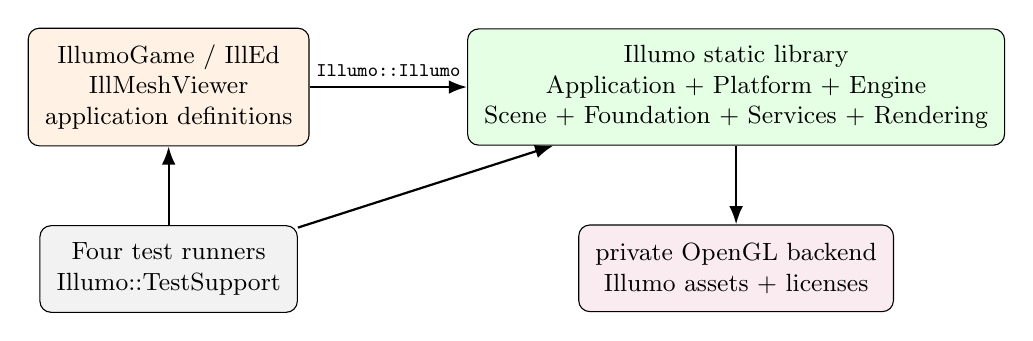
\begin{tikzpicture}[
  font=\small,
  box/.style={draw, rounded corners, align=center, inner sep=6pt, minimum height=1.1cm},
  arr/.style={-{Latex}, thick}
]
  \node[box, fill=orange!10] (game) {IllumoGame / IllEd\\IllMeshViewer\\application definitions};
  \node[box, fill=green!10, right=2.0cm of game] (lib) {Illumo static library\\Application + Platform + Engine\\Scene + Foundation + Services + Rendering};
  \node[box, fill=purple!8, below=1.0cm of lib] (gl) {private OpenGL backend\\Illumo assets + licenses};
  \node[box, fill=gray!10, below=1.0cm of game] (tests) {Four test runners\\Illumo::TestSupport};

  \draw[arr] (game) -- node[above]{\scriptsize \texttt{Illumo::Illumo}} (lib);
  \draw[arr] (lib) -- (gl);
  \draw[arr] (tests) -- (game);
  \draw[arr] (tests) -- (lib);
\end{tikzpicture}
\end{center}

\subsection{Runtime one-liner}
Illumo platform entry $\rightarrow$ \symbolref{CreateIllumoApplication}
$\rightarrow$ engine-owned \symbolref{RunIllumoApplication} applies supplied
product defaults and metadata-driven CLI $\rightarrow$ construct and fallibly
initialize \symbolref{Illumo} $\rightarrow$ register the supplied required product
module and engine-owned optional Debug module $\rightarrow$ \texttt{std::chrono} loop
\{\,\symbolref{update}, \symbolref{render}\,\} until window close.

\subsection{Non-goals (current)}
\begin{itemize}
  \item No install/export package, shared DLL, or stable binary ABI.
  \item No general-purpose AAA renderer, full ECS, or speculative framework.
  \item No SceneGraph serialization, retained UI, culling hierarchy, or update
        framework until a concrete consumer defines those contracts.
  \item No multiplayer or networking.
  \item No Linux support claim until native validation exists; macOS is not targeted.
\end{itemize}

\clearpage
\section{Source layout}
\label{sec:layout}

The canonical workspace is configured from the repository root. Responsibility
is divided between the reusable Illumo project and its products: IllEd,
IllMeshViewer and Playground in this repository, and the game, CSim (target
IllumoGame), in its own repository cloned into the ignored \pathref{CSim/}
folder (D-F5). The \pathref{CSim/} rows below exist only when it is cloned;
the engine configures, builds and passes its suite without it, and
\pathref{CSim/ENGINE\_MIN\_COMMIT} names the oldest engine commit the game builds
against.

\begin{center}
\begin{tabularx}{\linewidth}{@{}l X@{}}
\toprule
\textbf{Path} & \textbf{Role} \\
\midrule
\pathref{Illumo/Include/Illumo/} & Supported public library headers, included as \texttt{<Illumo/...>}. \\
\pathref{Illumo/Source/Engine/} & Host/module lifecycle, generic application runner, context, and Debug module. \\
\pathref{Illumo/Source/Scene/} & Persistent nodes, hierarchy, transform cache, subtree state, and render extraction. \\
\pathref{Illumo/Source/Foundation/} & Generic macros, build information, and compact implementation support. \\
\pathref{Illumo/Source/Services/} & Logging, environment, input, system CLI, generic console, and allocators. \\
\pathref{Illumo/Source/Rendering/} & Backend-neutral renderer plus private window/OpenGL implementation. \\
\pathref{Illumo/Source/Platform/} & OS entry points, native dialogs, and SaveLoad implementations. \\
\pathref{Illumo/Include/Illumo/Content/}, \pathref{Illumo/Source/Content/} & Optional \texttt{Illumo::Content} library (D-E18): \texttt{VirtualPath}, \texttt{PackageManifest}, \texttt{PackageArchive}, \texttt{VirtualFileSystem}, \texttt{PackageMounts}, \texttt{VfsAssetSource}, \texttt{VfsConsole}, \texttt{VfsTreeSource}, \texttt{SceneDocument}, \texttt{IlscCodec}, \texttt{SceneAssetRefs}, and \texttt{SceneInstance}. Core Illumo never includes it; guests link the mirror \texttt{IllumoGuestContent}. \\
\pathref{Illumo/tools/IllumoPack.cpp} & Host tool that packs a package directory into an \texttt{.ilpk} or verifies one. \\
\pathref{Illumo/Tests/} & Library-owned \texttt{Illumo.*} cases and private implementation tests. \\
\pathref{Illumo/Tests/Content/} & \texttt{Illumo.Content.*} cases and the \pathref{Fixtures/archive} package that CMake zips as a reader fixture. \\
\pathref{IllumoGuest/Include/IllumoGuest/} & Guest SDK, including \texttt{FileTree.h} (\texttt{GuestFileTree}), \texttt{VfsAssets.h} (\texttt{GuestVfsAssets}), and \texttt{SceneFetches.h} (\texttt{GuestSceneFetches}). \\
\pathref{Illumo/TestSupport/Include/} & Test-only \texttt{Illumo::TestSupport} headers, including MockBackend. \\
\pathref{CSim/Source/Game/} & Application definition, CA defaults, canvas, sparse simulation, editor, and game module. \\
\pathref{CSim/Source/Rulesets/} & Cellular-automata rules and palettes. \\
\pathref{CSim/Scenes/} & Packaged scenes; \pathref{render3d-test.ilsc} is the \texttt{render3dTest} diagnostic. \\
\pathref{CSim/Tests/} & Product-owned \texttt{IllumoGame.*} cases. \\
\pathref{IllEd/Source/}, \pathref{IllEd/Tests/} & World editor (document over \texttt{SceneInstance}, history, selection, shortcuts, gizmo, inspector, clipboard, asset browser) and \texttt{IllEd.*} cases. \\
\pathref{IllMeshViewer/Source/}, \pathref{IllMeshViewer/Tests/} & Mesh and scene viewer and \texttt{IllMeshViewer.*} cases. \\
\bottomrule
\end{tabularx}
\end{center}

\subsection{Related trees}
\begin{itemize}
  \item \pathref{Illumo/Shader/} and \pathref{Illumo/Assets/} are library-owned
        runtime data staged beside consuming applications by the supplied CMake helper.
  \item \pathref{Illumo/thirdparty/} holds vendored dependencies and licenses.
  \item \pathref{CSim/envvars.json} is product-owned default configuration
        and is seeded separately from library assets.
  \item \pathref{IllEd/illumo.json}, \pathref{IllMeshViewer/illumo.json}, and
        \pathref{CSim/illumo.json} are the package manifests staged
        into \pathref{apps/<name>/} (D-E22); \texttt{app.json} no longer exists.
  \item \pathref{archive/} is historical code and is not built.
  \item \pathref{docs/} is the canonical technical-documentation tree.
  \item Root and nested \texttt{AGENTS.md} plus \pathref{.agent/} are D-DOC2
        operational exceptions, not architecture sources.
\end{itemize}

\subsection{Naming landmine (Windows)}
\begin{decisionbox}[title={Decision: MathTypes.h (2026-07-28)}]
Do \textbf{not} put a header named \pathref{Math.h} on a case-insensitive include
path. MSVC resolves \texttt{\#include <math.h>} to it and breaks the CRT/GLM.
Project math aliases live in \pathref{Illumo/Foundation/MathTypes.h}.
\end{decisionbox}

\subsection{Include boundary}
Downstream code uses package-qualified public includes such as
\texttt{<Illumo/Engine/Illumo.h>}. IllumoGame receives no private
\pathref{Illumo/Source/} include root, and OpenGL implementation headers stay
private. A consumer-only compile smoke target continuously checks this boundary.
Products that load scenes or packages also link \texttt{Illumo::Content} and
include \texttt{<Illumo/Content/...>}, as does the WASM host
(\pathref{Illumo/Source/Wasm/}); the core static library never includes those
headers. Engine tools see the file tree only through the core interface
\symbolref{IFileTreeSource} (\pathref{Illumo/Services/FileTreeSource.h}).

\section{Runtime loop and program scenes}
\label{sec:runtime}

\subsection{In-game frame profiler}
\symbolref{FrameProfiler} is a main-thread, engine-owned 120-frame timing ring.
Sequential steady-clock marks partition each measured loop body into input,
camera, debug-overlay and program updates, draw-list preparation, asset
pumping, command generation/submission, backend presentation, frame limiting,
and remaining time.
The renderer can return the timestamp between submission and presentation;
ordinary untimed calls keep their previous behavior. GPU execution and concurrent
simulation workers are excluded. Disabled sampling performs no clock queries.

\symbolref{DebugOverlay} borrows the collector explicitly and owns a bounded
GameVisual pie with text. F6 or \texttt{profiler on} enables it; keys 1--3
drill into groups and 0 returns to Frame. Values refresh four times per second,
including resize and navigation updates. The console takes priority. Visible
profiler navigation captures both number events and held-key polling before
the program update. FPS and memory visibility remain independent. See
\pathref{docs/frame-profiler.md} and decision D-PROF1.

\subsection{Illumo application runtime}
\pathref{Illumo/Source/Engine/Application.cpp} owns the process around the
application: logger lifetime, the settings file, argument parsing mechanics,
the startup report, engine initialization and, when the window asks for it,
the relaunch. IllumoRuntime is the one application. Its definition in
\pathref{Illumo/Source/Wasm/RuntimeApplication.cpp} supplies declarative
metadata, a defaults callback and a \texttt{run} callback through
\symbolref{IllumoApplicationDefinition}:
\begin{lstlisting}
int RunIllumoApplication(int argc, char** argv,
                         IllumoApplicationDefinition application) {
  LoggerLifetime logger;
  Illumo illumo(/* application name + settings path */);
  application.applyDefaults(&illumo.environment());
  if (SysCmdLine::ParseCommandLine(argc, argv, &illumo.environment(),
                                   application.commandLine).shouldExit())
    return /* requested exit code */;
  if (!illumo.initialize()) return 1;
  const int exitCode = application.run(illumo, launched);
  illumo.shutdown();
  return exitCode; // relaunched afterwards if the window asked to restart
}
\end{lstlisting}
The engine-owned platform entry obtains the definition from
\symbolref{CreateIllumoApplication} and invokes this runner. No loop decision
depends directly on GLFW. Help/version and validation may return before
graphics initialization.

IllumoRuntime's \texttt{run} callback reads the launch options, mounts the
packages, builds one \symbolref{WasmProgram} for the launched package and
hands it to a \symbolref{RuntimeShell}
(\pathref{Illumo/Source/Wasm/RuntimeShell.cpp}). The shell owns the program,
the audio device the program borrows, the debug overlay, the paced loop, and
the \texttt{--capture} and \texttt{--bench-frames} runs:
\begin{lstlisting}
int RuntimeShell::run(std::chrono::steady_clock::time_point launched) {
  if (!start()) return exitCode(); // the program, then the overlay
  while (!closing()) {
    frame(/* steady_clock delta */);
    framePacer.pace(/* FPS cap, VSync, refresh rate */);
  }
  stop();                          // the overlay, then the program
  return exitCode();
}
\end{lstlisting}
No product supplies a native definition: IllumoGame, IllEd and IllMeshViewer
are WASM packages, and each is one program (\cref{sec:runtime-programs}).

\symbolref{FramePacer} limits the loop in software to the persisted
\texttt{fps} when VSync is off or \texttt{fps} is below the monitor refresh
rate, for example \texttt{fps 60} on a 144\,Hz display; \texttt{fps 0}
disables it. Each frame it sleeps on a \symbolref{PlatformWaitTimer} until the
timer's wake latency before the deadline, then spins with
\symbolref{PlatformCpuPause} for the remainder, about 0.5\,ms. A frame more
than 1.5 frame durations late resets the deadline rather than bursting to catch
up. On Windows the timer is a high-resolution waitable timer, so pacing does
not depend on the 1\,ms timer resolution that \symbolref{PlatformTimerScope}
requests and that Windows 11 ignores for occluded or minimized windows
(D-P34).

\subsection{Illumo host ownership}
\symbolref{Illumo} owns the long-lived generic services
(\symbolref{EnvVars}, \symbolref{RenderWindow}, \symbolref{Camera},
\symbolref{Renderer}, \symbolref{AssetManager}, \symbolref{CommandRegistry},
\symbolref{CommandLine}, \symbolref{InputManager}, \symbolref{DrawList}) and
the fixed parts of a frame. It owns no program. \symbolref{IllumoConfig}
carries only the application name and configuration-file path. Test-only
access injects the host's private window and backend factories.

Construction loads generic host defaults. The runner then invokes the product's
defaults callback and feeds its option descriptors to engine-owned
\symbolref{SysCmdLine} before fallible initialization. The window and backend
factories report failure; Illumo owns exactly one backend initialization attempt
and transfers the resulting \texttt{std::unique\_ptr<IBackend>} to the renderer.
Library code logs and returns failures rather than calling \texttt{std::exit}.
The window size persists as \texttt{WinX}/\texttt{WinY} (default
1280$\times$720). \symbolref{RenderWindow} records only positive sizes of a
window that is not minimized, so closing while minimized keeps the last
restored size, and initialization opens at the default, with a warning, when a
saved size is not positive.

\symbolref{IllumoContext} is a non-owning pointer bag frozen after successful
host initialization and passed to the program, its scenes and the debug
overlay when they start; each checks there that the fields it needs are set
(D-E5). \texttt{fileTree} is the one exception to the freeze: the program that
owns a file tree publishes it when it starts and withdraws it when it stops.
\texttt{scenes} points at a guest program's \symbolref{SceneDirector}; the
host leaves it null. The bag contains no game validation helpers or product
assumptions.

\subsection{Frame order, start and close (D-E31)}
\symbolref{Illumo} runs a frame in phases, and \symbolref{RuntimeShell} puts
the debug overlay and the one program between them:
\begin{enumerate}
  \item \texttt{Illumo::beginUpdate}: input, global hotkeys (F11, F3, F5) and
        the camera.
  \item \texttt{DebugOverlay::update}, in debug-tool builds only. It reads
        console keys before the program can drain them.
  \item \texttt{WasmProgram::update}.
  \item \texttt{Illumo::endUpdate}: unread key and character events are
        dropped, so they do not retrigger on the next update.
  \item \texttt{Illumo::beginRender}: the World-layer pipeline (motion blur)
        is configured and the drawables of the frame's \symbolref{DrawList}
        are cleared.
  \item \texttt{WasmProgram::dispatch}, then \texttt{DebugOverlay::dispatch},
        so console, diagnostics and renderer-demo drawables sit on top.
  \item \texttt{Illumo::endRender}: assets are pumped and the frame is
        rendered and presented.
\end{enumerate}
Every phase does nothing before \texttt{initialize} or after
\texttt{shutdown}.

\texttt{RuntimeShell::start} starts the program first, then the overlay, which
only debug-tool builds (Debug and RelWithDebInfo) compile (D-B1). A program
that fails to start fails the launch with exit code 1, and a capture or
benchmark caller still receives its JSON result. An overlay that fails to
start is logged and dropped. \texttt{RuntimeShell::stop} stops the overlay,
then the program. Whoever owns a program or a \symbolref{SceneDirector}
destroys it before \texttt{Illumo::shutdown}, because scene content holds
engine assets.

An interactive launch plays the engine splash, \texttt{GuiEngineSplash}
(D-UI14): the neon Illumo logo lights, holds and fades over the brand's dark
ground. The splash begins first while \texttt{WasmProgram::prepare} compiles
the program's modules into the compiled-code cache on a thread (D-E40); the
program starts between frames once its module is ready, and the last splash
frame holds if the compile outlasts the splash. The program is neither updated
nor drawn until the splash's last frame has shown, so its first scene enters
afterwards and no program triggers or waits for the splash. A later launch
finds the compiled code in \pathref{cache/wasm} beside the runtime and skips
the compiler; Vulkan and Direct3D 12 likewise keep compiled shaders in
\pathref{cache/gpu} (D-R38). Any key except Grave, or a fresh
click, skips it; the console stays usable, and a close during the splash ends
the run without asking the program. Capture and benchmark runs have no splash.

When the window asks to close, \texttt{RuntimeShell::closing} asks the program
(\texttt{WasmProgram::closeRequested}); inside the guest the question reaches
the active scene's \texttt{closeRequested}. A declined request calls
\texttt{Illumo::deferClose}, which cancels the window's close flag and drops a
restart riding on it, and the loop continues. A failed guest always agrees, and
a finished capture or benchmark closes without asking. IllEd shares its
Save/Discard/Cancel flow with native close and records approved discard so a
dirty document does not prompt repeatedly. Render windows implement close-flag
cancellation (\texttt{cancelCloseRequest}); the const
\texttt{Illumo::shouldClose} query has no callbacks.

\subsection{Programs and scenes (D-E31, D-R30)}
\label{sec:runtime-programs}
Each package is one WASM program that manages scenes; the engine has no module
registry. Inside the guest, a \symbolref{GuestProgram}
(\pathref{IllumoGuest/Include/IllumoGuest/Program.h}, in
\texttt{IllumoGuestContent}) composes a guest-local \symbolref{IllumoContext}
and lives as long as the WASM store. It owns what every scene shares
(settings, fonts, the product's catalogs and program-wide UI) and a
\symbolref{SceneDirector}. \texttt{createScenes(SceneDirector\&)} runs once
after bootstrap: it adds the program's scenes and switches to the first.
Returning false, or a first scene that fails to start, closes the product.
\texttt{updateProgram} and \texttt{dispatchProgram} carry program UI shared by
every scene: it updates before the active scene, so it takes input first, and
dispatches after it, so it draws on top. \texttt{updateOverlay} and
\texttt{dispatchOverlay} carry an overlay above everything, such as CSim's
software pointer. Each guest update applies a pending switch, runs queued
console commands, updates the camera, then the program UI, the active scene
and the overlay, and drops unread key and character events. Each guest frame
dispatches the active scene, then the program UI, then the overlay.

A \symbolref{ProgramScene}
(\pathref{Illumo/Include/Illumo/Content/ProgramScene.h}, also built into
\texttt{IllumoGuestContent}) is one screen of a program: its own logic, UI and
console commands, backed by a \symbolref{SceneInstance}:
\begin{lstlisting}
class ProgramScene {
public:
  virtual bool start(IllumoContext& context) = 0; // once, before first enter
  virtual void enter() {}                         // each time it is activated
  virtual void leave() {}                         // each time it is left
  virtual void update(double elapsed) = 0;        // only while active
  virtual void dispatch(DrawList& frame) = 0;     // only while active
  virtual void stop() = 0;                        // once
  virtual bool closeRequested() { return true; }
  virtual SceneInstanceOptions contentOptions() const { return {}; }
  SceneInstance& content();    // empty unless it loads a document
  IRenderWorld* world() const; // its render world, or null
};
\end{lstlisting}
\texttt{command(...)} registers a scene-scoped console command, withdrawn when
the scene leaves or stops. \texttt{dispatchContent} updates the content and
adds its drawable and sky to the World layer.

The \symbolref{SceneDirector}
(\pathref{Illumo/Include/Illumo/Content/SceneDirector.h}) owns a program's
scenes by name (\texttt{add}, \texttt{emplace}, \texttt{has}, \texttt{find},
\texttt{active}, \texttt{activeName}) and switches between them.
\texttt{switchTo(name, Cut)} applies at the next frame boundary; \texttt{Cover}
waits until the program reports its transition cover fully drawn
(\texttt{coverComplete}). A switch (\texttt{applyPending}) drains the key and
character queues and resets the frame's passes and drawables. The old scene
leaves: its camera is saved and its commands are withdrawn. The target starts
if it has not yet (content, render world, the camera the director was created
with), its saved camera is restored, and it enters. A target that fails to
start is logged and the previous scene re-entered. The scene left is kept,
frozen, and resumes where it was until the program releases it;
\texttt{release} refuses the active scene and a pending target. Only the
active scene updates, receives input and draws. \texttt{stopAll}, like the
destructor, stops the active scene first, then the others in reverse order of
adding.

With the \texttt{HostRender} capability, \texttt{GuestSceneWorlds}
(\pathref{IllumoGuest/Include/IllumoGuest/SceneWorlds.h}) gives each scene its
own \texttt{GuestRenderWorld} on the host (frame schema v8, D-R30), and
\texttt{IllumoContext::camera} and \texttt{renderWorld} follow the active
scene. A kept scene's world stays on the host, intact and undrawn, and steady
frames send nothing. A guest has at most 8 worlds; a scene started beyond that
has none and draws its lit meshes as \symbolref{MeshVisual}s, as every scene
does with \texttt{hostRenderWorld=0}. Crossfades between scenes are deferred,
and a camera per world waits for them.

CSim's program has two scenes, the title screen and the canvas, and keeps the
canvas across trips to the title. IllEd is one
\texttt{EditorScene} whose \texttt{EditorDocument} edits the scene's content.
IllMeshViewer is one \texttt{MeshViewerScene} whose content is the opened
document. \pathref{Templates/SpinningCube}, the template for new projects, is a
\texttt{GuestProgram} with one \texttt{SpinningCubeScene} and a
\texttt{cube\_speed} scene command. Design and milestones:
\pathref{docs/scene-programs-design.md}.

\subsection{Frame flow (conceptual)}
\begin{center}
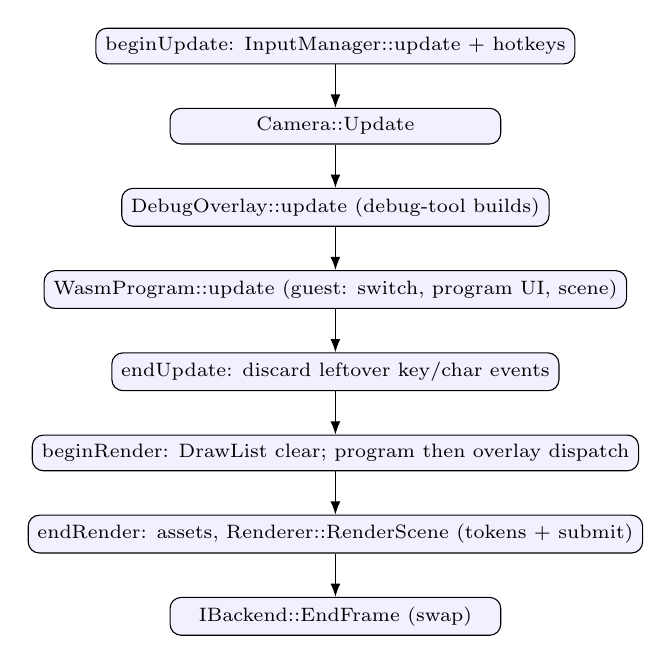
\begin{tikzpicture}[
  font=\scriptsize,
  node distance=0.55cm,
  flowstep/.style={draw, rounded corners, align=center, fill=blue!6, minimum width=4.2cm},
  arr/.style={-{Latex}}
]
  \node[flowstep] (1) {beginUpdate: InputManager::update + hotkeys};
  \node[flowstep, below=of 1] (2) {Camera::Update};
  \node[flowstep, below=of 2] (3) {DebugOverlay::update (debug-tool builds)};
  \node[flowstep, below=of 3] (4) {WasmProgram::update (guest: switch, program UI, scene)};
  \node[flowstep, below=of 4] (5) {endUpdate: discard leftover key/char events};
  \node[flowstep, below=of 5] (6) {beginRender: DrawList clear; program then overlay dispatch};
  \node[flowstep, below=of 6] (7) {endRender: assets, Renderer::RenderScene (tokens + submit)};
  \node[flowstep, below=of 7] (8) {IBackend::EndFrame (swap)};
  \foreach \a/\b in {1/2,2/3,3/4,4/5,5/6,6/7,7/8} \draw[arr] (\a) -- (\b);
\end{tikzpicture}
\end{center}

\symbolref{RenderWindow} defaults to swap interval one. Persisted
\texttt{vsync=0} selects uncapped profiling, while Debug metrics distinguish
paced swap completions from CPU submissions.

The global F11 shortcut switches between a normal window and a fullscreen
window, and returns an exclusive fullscreen window to a normal window. The
window publishes the resulting display mode to EnvVars, and the host reports
that value without changing it again. A rejected toggle preserves the prior
setting. The fullscreen window covers the monitor without a video-mode
switch. Exclusive fullscreen gives the monitor to the window at the current
mode and refresh; that path drops the OpenGL swap wait on Windows, and a
later interval call does not restore it.

IllMeshViewer consumes queued Press events for O (open), F/R (reset camera),
G (grid), X (wireframe), and B (skybox). Hold/repeat and release events do not
execute these actions. Shortcuts are suppressed while the console is open;
unrelated keys remain available to the host. No shortcut latch is shared
between viewer instances.

IllEd body selection records the initial hit offset on the same constraint plane
used during dragging. Holding or releasing an off-center click without moving
does not translate the object or dirty the document. If the initial drag-plane
intersection fails, selection still succeeds but dragging does not begin.

In 3D, IllEd selects the nearest forward screen-ray intersection with an
object's transformed local bounds. Parent transforms, nonuniform scale and
rotation are included; inherited hidden/disabled state excludes candidates.
Singular or nonfinite bounds are skipped. Bounds follow attachment recipes,
with a small proxy for empty nodes; equal-distance ties prefer later document
entries. This is bounds-based picking, not triangle-exact picking. 2D picking
and ground-plane placement retain their existing paths. A 3D selection ray
need not intersect the ground plane.


\subsection{Process memory diagnostics}
In debug-tool builds, \symbolref{DebugOverlay} composes FPS and memory as plain
white text with a one-pixel black glyph backing on a semi-transparent black
rectangle, plus a frame-time line under the FPS block. F3 and \texttt{fps}
control only FPS;
\texttt{memory [on|off|toggle]} controls the persisted \texttt{showMemory}
flag, initially off. Each section may be visible independently. The memory
rows show current working set, process-lifetime peak working set and private
committed memory in MiB with one decimal place. Working set includes shared
pages; private commit need not be resident. These are whole-process values,
not GPU memory or allocation/leak tracking.

The internal presentation state maintains independent refresh clocks. Memory
is queried immediately on enable, then once per second while visible; unchanged
text does not rebuild the drawable. The platform-neutral memory query returns
byte counts and availability. Windows obtains them through the process-memory
API; unsupported scaffolds and failures display ``Memory: unavailable'' and
retry at the normal interval. Native headers stay in the Windows platform
implementation. No worker or new rendering path is introduced.
\subsection{Input registration retirement (2026-09-11)}
InputManager bounds live contexts to 32, reuses released slots and issues distinct
manager-local IDs. Invalid activation preserves selection; active retirement
selects neutral input. CellGameModule releases its registration on Exit and
rejects exhausted startup before allocating domain state. Repeated module entry
must not consume permanent input slots.

Registration accepts at most one required module and closes when startup completes.
The first pending non-null transition is retained; later requests log rejection.
Destructors do not invoke module lifecycle callbacks. Dense compatibility tests
are independent of this product-neutral runtime.

Note (2026-09-26): D-E31 removed module registration and transitions, so the
second paragraph above is history. \texttt{CanvasScene} registers its input
context in \texttt{start}, still rejecting exhaustion before allocating domain
state, releases it when it leaves or stops, and registers it again when it
enters.

\section{Rendering --- current state}
\label{sec:rendering-current}

\begin{statusbox}
\textbf{Illumo ships world meshes, painter-correct 2D composition, cubemaps,
and explicit offscreen passes.} Live
frame path is acquire/enroll + tokens + submit via
\symbolref{Renderer}/\symbolref{IBackend}.
Drawables emit tokens through \texttt{AppendCommands}; GL draw submission is
confined to private \pathref{Illumo/Source/Rendering/OpenGL/} (plus window
bootstrap), Vulkan's to \pathref{Illumo/Source/Rendering/Vulkan/} (D-R33) and
Direct3D 12's to \pathref{Illumo/Source/Rendering/D3D12/} (D-R36, Windows),
chosen per launch. Headless \pathref{Illumo/TestSupport/Include/Illumo/Testing/MockBackend.h}
powers \texttt{IllumoTests}. CanvasView
presentation is \textbf{a padded camera cache + bounded CPU RGB fade + one RGB
display texture/quad} with tiled multi-rect uploads (see canonical note in
\pathref{docs/architecture-consensus.md}).
OpenGL, Vulkan and Direct3D 12 execute the same tokens with the same
results.
\end{statusbox}

\subsection{What actually draws frames today}
\begin{enumerate}
  \item The program, then the debug overlay, dispatch into the frame's
        \symbolref{DrawList}, adding \symbolref{DrawableBase*} pointers to its
        \textbf{layers} (\texttt{World} CanvasView, \texttt{UI} console/splash,
        \texttt{Debug} FPS). In a guest, the active program scene's
        \texttt{dispatch} fills the guest's own list.
  \item \symbolref{Illumo::endRender} pumps completed managed asset work, then
        drives \symbolref{Renderer}:
        \texttt{BeginFrame} $\rightarrow$ \texttt{RenderScene} $\rightarrow$
        \texttt{EndFrame} (swap).
  \item \symbolref{Renderer::RenderScene}:
        initial screen clear + viewport tokens; walk layers
        World $\rightarrow$ UI $\rightarrow$ Debug, using each layer's effective
        custom passes or ordinary screen rendering; each drawable
        \texttt{AppendCommands}; if a drawable returns false, legacy immediate
        \texttt{Draw()} still runs (hybrid fallback; production drawables return true).
        It captures window dimensions and the primary camera MVP once for that
        extraction; matching \symbolref{GameVisual} emitters reuse those values.
  \item \symbolref{IBackend::SubmitCommandQueue} $\rightarrow$
        \symbolref{GLDevice::ExecuteCommandQueue} resolves handles and issues GL.
\end{enumerate}

\subsection{Compiled scene extraction (D-E12/D-R25)}
The per-frame \symbolref{DrawList} (named \texttt{Scene} until D-E31) stays a
non-owning drawable list.
\symbolref{SceneGraph} owns persistent SoA slots and intrusive hierarchy links,
with graph-local generational handles. Structural edits lazily compile a
preorder, parent indices, and subtree ranges. Local TRS edits set one dirty bit
and lower a watermark; one forward pass resolves affected world transforms.
World queries walk ancestors without consuming compiled dirtiness. Matrix
input decomposes to TRS; shear and projective matrices are lossy.

Nodes hold interned nonunique names, opaque 64-bit payloads, and ordered borrowed
attachments. Bounds cache by nonzero attachment revision; zero requests polling.
World boxes transform each attachment before union, and backward refit computes
subtree boxes. Unknown bounds fail open. A lazy binned-SAH query index has a
linear correctness fallback; warm queries still poll revisions in linear time.
Bounds-only changes on an unchanged structure refit the index's node boxes in
one reverse pass instead of rebuilding it; structural changes, and changes
after 64 consecutive refits, rebuild (D-E41).
The 4,096-entry change journal reports overflow explicitly.

\texttt{SceneGraphDrawable}, not the graph, derives from
\symbolref{DrawableBase}. It obtains one immutable snapshot per renderer frame
and consumes its matrices, bounds, and attachment pointers for collection,
depth, and color. Two graph-owned buffers are reused; ring reuse, attachment
invalidation, destruction, and graph teardown expire views. The adapter checks
the view before each callback. Owners invalidate before changing or retiring
borrowed content and preserve emitted token payloads until submission returns.
Mutation during extraction is rejected. All callbacks remain main-thread affine.

The shared shadow fit follows caster collection. Camera-missed subtrees skip
camera tests but retain potential off-camera casters, and depth relevance uses
snapshot bounds after fitting. This resolves the proposal's early-shadow-flag
assumption without changing the renderer's shadow policy. The temporary
\texttt{sceneSnapshotExtraction=0} switch selects guarded direct traversal.

Sibling order is part of the contract (D-E26):
\texttt{setParent(node, parent, insertBefore)} places a node immediately before
a current child of \texttt{parent}, or last when \texttt{insertBefore} is null,
and \texttt{getPreviousSibling} complements \texttt{getNextSibling}. The cycle
check and Reparented change record apply as for any reparent, and an unchanged
position records nothing. Scene documents store nodes in graph preorder, so
sibling order round-trips, and undo can restore a deleted node to its exact
position.

\subsection{SceneInstance (D-E18/D-E19)}
Scenes reach the renderer through \symbolref{SceneInstance} in
\texttt{Illumo::Content}, not through product code. It owns the document
state, one \symbolref{SceneGraph}, one \symbolref{MeshVisual} per renderable
component, and the asset references those visuals hold; stable node ids are
graph names. Each program scene owns one as its \texttt{content()} (D-E31). A
scene adds \texttt{drawable()} (and \texttt{skybox()} when the environment
names one) to the frame's \symbolref{DrawList} and calls \texttt{update()} once
per frame; \texttt{ProgramScene::dispatchContent} does both. Per-node edits (transform, flags, components, reparent with sibling
position, create, remove) validate first, change only the nodes they touch,
and invalidate graph snapshots before reconfiguring an attachment; recolors
and resizes that keep a node's component kinds reconfigure the visual in
place.
\begin{itemize}
  \item \textbf{Primitives:} solid shapes (rect, ellipse, triangle, cube,
        pyramid, sphere) share one immutable unit mesh per shape and instance,
        enrolled through \texttt{AssetManager::acquireMesh(MeshData)}; the
        primitive extent is the visual's model scale and its color the tint.
        Wire cube and wire sphere stay procedural.
  \item \textbf{Assets:} mesh, texture, atlas, and cubemap assets load through
        \symbolref{AssetManager} by normalized virtual path. A missing or
        failed asset draws a magenta placeholder and records a warning the
        program can read (\texttt{warnings()}).
  \item \textbf{Lighting:} the first enabled, visible \texttt{light} component
        in preorder supplies the one directional light; otherwise the
        environment sun does. Ambient color and shadow settings are pushed
        into every visual. 2D scenes are unlit.
  \item \textbf{Skybox:} the environment's cubemap asset is drawn by a
        \texttt{SkyboxVisual} that is a separate drawable, not a graph node.
        \pathref{SkyboxVisual.cpp} moved into the shared guest engine so
        every guest can use it.
  \item \textbf{Picking:} \texttt{pickRay} tests attachment local bounds from
        \texttt{SceneGraph::raycastCandidates} with rotation, scale and
        effective visibility, preferring the later node in preorder on ties
        (drawn on top in 2D). Optional pick proxies give empty, light and
        camera nodes a selectable box.
\end{itemize}
Loading 2,000 nodes takes about 3.8\,ms and 1,000 batched transform edits
about 0.8\,ms in Release (\texttt{Illumo.Content.Bench.Instantiate2000}).

IllEd's \texttt{EditorDocument} edits its \texttt{EditorScene}'s content, one
\texttt{SceneInstance}, and is the only mutation gateway; the editor adds no
per-node attachments. IllMeshViewer
opens scenes through the same class, and IllumoGame's \texttt{render3dTest}
diagnostic is \pathref{CSim/Scenes/render3d-test.ilsc} instantiated by
it. Journal overflow resynchronizes bindings without rebuilding nodes. Capture
fixtures use the adapter; CA storage and UI remain separate. See
\pathref{docs/scene-graph-v2-design.md},
\pathref{docs/scene-graph-v2-plan.md}, and
\pathref{docs/content-packages-and-scenes-design.md} for evidence and gated
follow-ups.

\subsection{Layers, styles, and drawables (D-R14, D-R18)}
The initial clear explicitly selects the screen framebuffer and full-window
viewport. Each ordinary layer reestablishes that target and viewport before
its drawables, including after an offscreen custom pass. The OpenGL binding
cache starts unknown on each submission, so the first screen bind is issued
even if the preceding submission left an offscreen framebuffer active.
Pass color and depth clear flags are independent. Color-only passes emit a
color-buffer clear; depth clears carry the requested value. Combined pass
clears emit both commands. Clear tokens default to depth one, so a later
default clear does not inherit a custom value from a previous pass.

\symbolref{DrawList} stores host default passes separately from application
overrides. Nonempty application overrides take precedence, whether installed
in a scene's \texttt{start}, \texttt{update}, or \texttt{dispatch}. The host
updates only defaults through \texttt{SetDefaultLayerPasses}, so motion-blur
toggles and parameter changes cannot erase application passes. An empty
override, \texttt{ClearLayerPasses}, or \texttt{ResetDefaultPasses} restores
the current host fallback; without one, rendering uses the ordinary screen
draw. \texttt{passesIn} and \texttt{hasCustomPasses} describe the effective
sequence. A scene switch resets all application overrides and clears the
frame's drawables before the old scene leaves, detaching borrowed callbacks
while preserving defaults.
\begin{itemize}
  \item \textbf{Layer} --- ordered composition bucket, rendered to the screen
        by default or through its effective custom pass sequence.
  \item \textbf{RenderStyle} --- Renderer-owned generational registry: shader handle +
        \texttt{PipelineState} defaults (\texttt{Canvas}, \texttt{UiText},
        \texttt{Console}, \texttt{Shape}, \texttt{Sprite}). Canonical Shape/Sprite
        programs consume \texttt{uMVP} only (\symbolref{WorldLook}). Overlay
        chrome supplies a Y-down screen ortho; world objects supply camera
        view-projection times node world. GPU programs still live in backend
        registries.
  \item \symbolref{DrawableBase} --- type-erased list entry; virtual
        \texttt{Draw} + virtual \texttt{AppendCommands} (default returns false).
        \textbf{No GL handle ownership} on the base (D-R6). Content handles
        only; call \texttt{bindStyle} then emit content tokens.
  \item \symbolref{Drawable<Derived>} --- CRTP: \texttt{Draw} $\rightarrow$
        \texttt{DrawImpl} for the rare immediate path. Production emitters
        (CanvasView, CommandLine, GLString/SplashText) use
        \texttt{AppendCommands} only; \texttt{DrawImpl} is empty/no-op.
  \item \symbolref{GameVisual} (D-R15) hosts composed
        shape/sprite/text values. Parent and local \texttt{Transform2D},
        normalized pivots, atlas regions/flips, and integer draw order build one
        stable cross-type stream. A run of one style, texture and kind joins
        the latest earlier batch with that key when nothing drawn in between
        overlaps it (D-R34), so a list of widgets (background, icon, label
        each) draws as a few batches while every pixel keeps its painter-order
        sequence of writes; there is no global texture sort. Shapes without
        a custom style draw as sprites of the renderer's white texel, so
        shapes, sprites and text share one pipeline (D-R35); a visual of more
        than 64 items that are all shapes, and guest recordings, keep the
        shape mesh.
        Pixel-space rebuilds conservatively reject quads outside the logical
        viewport. An optional top-left logical-pixel clip rejects fully
        excluded quads before upload and uses nested, intersected scissor
        tokens for partial content; popping the clip restores any outer
        scissor (D-R23). World-space behavior is unchanged.
        Dynamic buffers reserve 1,024 quads, double as needed, and stop at a
        configurable 65,536 default ceiling.
  \item \symbolref{MeshVisual} (D-R21/D-R24) is the world mesh host and
        \symbolref{ISceneRenderAttachment}: colored lines/triangles, textured
        quads (sprites), optional camera-facing billboards, optional
        directional lighting with participation in a scene-level depth-only
        shadow pass, and optional object motion blur from the previous clip
        pose. Bounds cover every geometry source immediately after mutation;
        camera-facing sprites use a view-independent enclosing volume. It clones
        Shape/Sprite styles with depth-tested pipelines and emits
        \texttt{uMVP}. Lit meshes also emit \texttt{WorldLook} light, shadow,
        and motion-blur uniforms from CPU-side drawable state; products
        persist those values through EnvVars rather than having
        \symbolref{MeshVisual} read configuration.
        One host can contain multiple visual items. Use child scene nodes for
        independent transforms and subtree state; each node may borrow an ordered
        list of attachments. Overlay HUD stays on \symbolref{GameVisual}. Dynamic
        procedural meshes upload dirty vertices through \texttt{UpdateBuffer};
        capacity growth replaces the backing allocation. Immutable imported
        meshes instead borrow one reference-counted \texttt{MeshHandle} from
        \symbolref{AssetManager}; multiple visuals reuse the upload while
        retaining independent transform, tint, lighting, and motion state.
        The Renderer retains caster descriptors, chooses light settings from
        the first camera-visible caster, and filters them against a conservative
        camera-frustum extrusion toward the light. Invalid reconstruction falls
        back to all casters. A monotonically increasing frame serial resets
        previous-MVP history when a culled visual re-enters.
\end{itemize}

\subsection{Managed assets (D-R17/D-R24)}
Shared fonts cache one atlas handle per live renderer ownership identity,
not per raw renderer address. The identity is weak in the font cache; expired
entries are pruned and explicitly retired texture handles are reenrolled.
Alternating live renderers reuses their separate enrollments. Renderer teardown
invalidates the identity before backend teardown; GPU ownership stays with the
backend, and a font never dereferences a retired renderer.

\symbolref{AssetManager} caches canonical file paths plus loading options and
returns stable typed handles. Duplicate acquisition increments a reference
count; the final release destroys the backend resource. Initial pending or
failed 2D texture/shader requests retain a checkerboard or fallback shader that follows
the documented custom-2D binding contract. One owned worker performs file reads
and stb decoding; \texttt{pump} applies GPU
replacement on the render thread before frame submission. Failed reloads keep
the last good object and record an error. Debug builds poll timestamps every
500\,ms and coalesce requests; explicit reload is available in all builds.
Shutdown cancels obsolete results and joins the worker before backend teardown.

Static mesh acquisition is synchronous and main-thread affine. The
\symbolref{MeshLoader} converts a file to CPU \texttt{MeshData};
\symbolref{AssetManager} canonicalizes the file path plus geometry-affecting
options, enrolls one immutable backend mesh, and returns its typed handle.
Duplicate acquisition increments a reference count and final release destroys
the backend resource. In-memory mesh data can be enrolled once and explicitly
retained for multiple consumers. Managed mesh metadata supplies the immutable
vertex/index counts and bounds needed by drawables. Mesh hot reload, materials,
and automatic instance aggregation remain outside this milestone.

The byte source is an \texttt{IAssetSource}: the file system natively,
\texttt{VfsAssetSource} over the host file tree in tools and native tests, and
\texttt{GuestVfsAssets} in guests, where canonical keys are normalized
absolute virtual paths (D-E24). \texttt{AssetManager::assetSource()} exposes
the source so a product can read a scene through it. MTL libraries beside an
OBJ resolve through the same source: \texttt{MeshLoader::materialLibraryNames}
is the single \texttt{mtllib} scanner, \texttt{AssetManager::acquireMesh}
reads each named library relative to the OBJ, and the text reaches the loader
as \texttt{MeshLoadOptions::materialText}. Materials are parsed but still not
bound.

Cubemaps retain their source kind and all canonical face paths (or the cross
path). Initial acquisition remains synchronous; reload decoding uses the same
CPU job path and publishes all six RGBA faces through cubemap replacement.
Initial success has revision one. Explicit path reload and timestamp polling
observe every face. Decode timestamps are captured before reading, so a later
edit remains observable on the next poll. Missing/mismatched faces or rejected
replacement keep the prior ready resource and revision. Cross extraction and
orientation are shared by initial load and reload; texture kinds cannot change
during replacement.

\subsection{CanvasView presentation (bounded RGB fade + dirty rects)}
\label{sec:canvas-rgb-fade}
\begin{itemize}
  \item Domain: \symbolref{SparseCellGrid} stores signed-coordinate
        16$\times$16 chunks and changes its revision only for a cell-content
        change. The view visits only chunks intersecting its camera source
        bounds.
  \item View: visible diagnostics are separate from a globally aligned cache
        padded by two 16-cell chunks on every side. Motion inside the cache
        changes only the camera MVP. CPU palette via \texttt{evalCell}
        $\rightarrow$ \texttt{targetRgb};
        \texttt{displayRgb} eases toward targets, newly revealed cells snap,
        and packed RGB is staged for upload. Unchanged grid, palette, and
        camera bounds skip resampling entirely.
  \item Zoom: normal views retain one nearest-filtered texel per 16$\times$16
        world cell. Far views use a stable integer density LOD bounded to about
        four screen pixels per texel; it coarsens immediately to fit and refines
        only when the next level fits within 80\% of the budget. Changed chunks
        map to deduplicated exact or overview cache bins. Exact texels are
        written from the chunk cells already in hand, and incremental overview
        bins accumulate only the chunks under them, falling back to one
        occupied-chunk walk past half the spanned chunks (D-P37).
  \item GPU: one reusable nearest-filtered RGB display texture and one
        world-space quad aligned to the same 16$\times$16 cell bounds as the
        editor cursor. Dirty 16$\times$16-texel tiles merge into at most eight
        \texttt{UpdateTexture} rectangles when their area is at most half the
        enclosing AABB; otherwise the AABB is submitted. Small dimension
        increases reserve 50\% texture headroom. Re-enrollment destroys the
        prior GL texture, PBOs, and fences under the same handle, and view
        destruction explicitly releases the texture. Upload-run and output-rect
        scratch vectors are retained across dirty frames.
  \item Shader/style: \symbolref{CanvasView} composes a world-space
        \symbolref{GameVisual} sprite and therefore uses the Renderer-owned
        inline \texttt{Sprite} style with sampler \texttt{uTexture}.
        The file-backed \texttt{Canvas} style and
        \pathref{Shader/canvas\_*.glsl} remain enrolled but have no production
        CanvasView binding.
  \item History: D-P4 briefly used GPU R8 + $256\times 1$ palette (snap colors).
        Fade was restored; dirty-rect PBO + bind-state tracker from that work
        remain. Canonical write-up:
        \pathref{docs/architecture-consensus.md} \S5.6.
\end{itemize}

\subsection{Instancing, recorded lists and RenderWorld (D-R28, D-R30)}
\begin{itemize}
  \item Buffers: backends may create generational instance and uniform
        buffers (\texttt{BufferHandle}, \texttt{IBackend::CreateBuffer}); the
        defaults return an invalid handle so recording and test backends need
        no change. Tokens \texttt{WriteBuffer}, \texttt{BindUniformBuffer},
        \texttt{SetInstanceStream} and \texttt{DrawIndexedInstanced} fill and
        use them. Instance attributes occupy locations 4--12
        (\texttt{InstanceLayout::LitModelTint}: model, previous model, tint;
        144 bytes).
  \item Frame block: \symbolref{Renderer} writes one std140
        \texttt{FrameUniforms} block (view-projection, previous
        view-projection, light space, shadow state) the first time a drawable
        calls \texttt{useFrameUniforms()} in a \texttt{RenderScene}. The
        instanced styles \texttt{LitMeshInstanced} and
        \texttt{ShadowDepthInstanced} (\pathref{Shader/mesh\_lit\_instanced\_*.glsl},
        \pathref{Shader/shadow\_depth\_instanced\_vertex.glsl}) read it and
        otherwise match the lit and shadow-depth math.
  \item Recorded lists: \texttt{RecordedCommandList} tokens are recorded once
        through the ordinary push helpers and run in place by one
        \texttt{ExecuteList} token per list. A list owns its matrices, refuses
        nested lists, has its own ceiling, and is counted per frame.
  \item \texttt{RenderWorld}: a World drawable owning persistent instances,
        materials and one environment behind \texttt{IRenderWorld}. Instances
        sharing a mesh range and material draw with one instanced call per
        pass. Per frame it culls against the camera and shadow volume,
        streams visible instances and patches counts; its lists re-record only
        when buffers, materials or the environment change. A bucket whose
        instances are unchanged and whose cull revision (Renderer's
        \texttt{getCullRevision}, \texttt{getShadowCullRevision}) holds skips
        culling, and an unchanged visible list skips the instance write
        (D-R39): a static 50,000-instance world went from 2.6\,ms to about
        1\,$\mu$s a frame. With a mock
        backend, 2,000 objects cost 0.11\,ms and 30 tokens per frame against
        3.8\,ms and 50,017 tokens as one MeshVisual each. On a real GPU its
        images are bit-identical to MeshVisual's, shadows included.
        \symbolref{SceneInstance}\texttt{::setRenderWorld} puts a scene's
        mesh-asset visuals into it (IllMeshViewer, IllEd, the game's 3D mode).
        It can also draw a sky (\texttt{setSkybox}) first, rebuilding the
        rotation-only view projection from the frame camera
        (\pathref{docs/host-render-world-design.md}).
  \item Worlds per scene (D-R30): frame schema v8 addresses host render
        worlds. \texttt{SelectWorld} (10) sends the world operations after it
        to a world id, created on first use; \texttt{ShowWorld} (11) picks the
        world that draws (0: none); \texttt{DestroyWorld} (12) releases one
        and everything in it. A version 7 frame is exactly ``world 1, shown''.
        A guest has at most 8 worlds, material and instance ids are per world,
        and the shown world draws with the frame camera. The guest SDK's
        \texttt{GuestSceneWorlds} gives every program scene its own
        \texttt{GuestRenderWorld}, so a kept scene's objects stay on the host
        undrawn and steady frames send nothing. \texttt{hostRenderWorld=0}
        still gives scenes no world.
\end{itemize}

\subsection{Host-retained 2D visuals (D-R29)}
\begin{itemize}
  \item \texttt{VisualStore}: 2D visuals by id, each a
        \symbolref{GameVisual} edited in place (items by index, opacity). A
        visual's draw tokens are recorded once and replayed with
        \texttt{ExecuteList} until its geometry or frame state (resolution,
        projection, clip) changes. \texttt{GameVisual::prepareFrame} builds
        and uploads; \texttt{emitDraws} pushes only clip and batch tokens.
  \item Guests: \texttt{GameVisual::AppendCommands} offers the visual to
        \texttt{IBackend::AppendVisual}, and \texttt{SkyboxVisual} to
        \texttt{AppendSkybox}. The guest recorder sends visual operations
        (frame schema v7 and later; only unconfirmed changes) and per-target
        compositions,
        and the host draws them through \texttt{VisualStore} in painter order
        between the remaining batches. Visuals that cannot travel, the canvas
        quad and the MeshVisual line overlays still record retained batches.
\end{itemize}

\subsection{Backend surface}
\symbolref{IBackend}: lifecycle and command-queue push/submit/clear. Resource
creation returns non-convertible slot+generation \texttt{MeshHandle},
\texttt{ShaderHandle}, and \texttt{TextureHandle} values. Validated
replace/destroy/query operations and command resolution reject stale handles
with a warning and safe no-op.

\symbolref{CommandQueue}: vector storage reserves 2,048 tokens, grows to a
configurable 65,536 default safety ceiling, and reports high-water and rejected
counts. Rejection logs once per reset interval. On the supported 64-bit Windows
build each token is 72 bytes. Matrix-uniform values are copied into retained
renderer-owned chunks of 128 matrices and the compact token borrows that stable
value until synchronous submission returns; the chunks reset after submission
and are reused by later frames. Matrix side storage uses a matching default
65,536-value safety ceiling so rejected token storms cannot grow it without
bound.

\symbolref{RenderCommand}: tagged union (\texttt{CommandType} + POD payload)
including pipeline, bind, uniforms, \texttt{UpdateTexture}, \texttt{UpdateBuffer},
clear, draw, and explicit enabled/disabled scissor state (D-R1).

Each \symbolref{GLShaderProgram} owns its uniform-location cache. Cache hits use
the token's name directly rather than building and hashing a combined
program-ID/name string, and shader replacement or destruction retires cached
locations with the owning program.

Uniform tokens carry a \texttt{UniformKey} (FNV-1a of the whole name) in
\texttt{RenderCommand::uniformKey}, set once by the \symbolref{Renderer} push
helpers; it occupies what was tail padding, so the token stays 72 bytes. OpenGL
locations and the Vulkan and Direct3D 12 program uniform slots resolve through
\texttt{UniformNameTable} by key and name, so no backend hashes a name string
per token; a key that disagrees with its name falls back to the derived key
(D-R37).

\symbolref{GameVisual}\texttt{::emitDraws} tracks the bound style, mesh and
texture and sends resolution, \texttt{uMVP} and the sampler unit once per
style per call, so a batch that shares its neighbour's style emits only its
texture (when it differs) and its draw (D-R39).

Renderer maintains a per-frame scissor stack for \texttt{pushClipRect}/
\texttt{popClipRect}. Nested clips intersect in physical viewport coordinates
and restore the prior state; low-level \texttt{pushScissor} remains the explicit
state-token path (D-R23).

\symbolref{GLTexture::UpdateSubImage}: rectangles through 64\,KiB use direct
\texttt{glTexSubImage2D}. Larger uploads select a signaled slot from a
three-PBO/\texttt{GLsync} ring without waiting; all-busy and map-failure cases
fall back to the direct path. Replacement/destruction deletes every fence and
buffer and retains the OpenGL 3.3 baseline.

Uploads reject invalid bounds, channel counts, row strides, and byte-size
overflow before any staging or GL call. Uploads bind on texture unit zero,
matching the device cache, and restore the caller's active unit and unpack
state. Cubemap file decoding explicitly produces RGBA for every face and cross;
raw two-channel cubemaps are rejected instead of reinterpreted as RGBA. OBJ
conversion validates all attribute references before publishing mesh data.

\symbolref{GLDevice}: bind-state tracker (skip redundant program/VAO/texture/
viewport within a submit); uniform location cache; blend-func-on-enable (D-R5).

Presentation defaults to monitor synchronization through
\texttt{glfwSwapInterval(1)}. The persisted \texttt{vsync} value selects that
frame-paced mode or an explicit uncapped profiling mode and may change live at
a swap boundary. Debug labels swap-completion cadence as \texttt{Paced FPS} and
main-loop work as \texttt{Submit FPS}; uncapped mode reports paced FPS as off
instead of treating thousands of CPU submissions as displayed frames (D-P32).

\subsection{Vulkan backend (D-R33)}
\texttt{Rendering/Vulkan/} is a second complete \symbolref{IBackend}. The
\texttt{GraphicsAPI} setting (\texttt{OPENGL} by default, or \texttt{VULKAN};
also \texttt{--graphics-api} and the console \texttt{set}, applied at the next
launch) picks the window and backend in \texttt{Illumo::initialize}; if the
Vulkan window or backend cannot start, the host logs why and starts OpenGL
instead, keeping the preference. The window for Vulkan is created with
\texttt{GLFW\_NO\_API}; everything else about it is unchanged.

The backend executes the same tokens and compiles the same GLSL 330 text, with
the OpenGL backend's observable results:
\begin{itemize}
  \item Every image, including a stand-in for the default framebuffer, is
        stored bottom row first and drawn with an unflipped viewport, so
        \texttt{gl\_FragCoord}, viewport, scissor and readback numbers match
        OpenGL; presentation blits the image to the swapchain flipped. Front
        faces are inverted and vertex shaders remap clip $z$ from $[-w,w]$.
  \item glslang compiles the shaders at run time under Vulkan's relaxed GLSL
        rules: loose uniforms form a per-program default block whose values
        persist as OpenGL program uniforms do, samplers and blocks are bound
        automatically, and varyings are matched by name.
  \item OpenGL's state machine is kept per device: texture units, uniform
        binding points, pipeline state, viewport and scissor persist; a mesh's
        instance stream stays attached as a VAO keeps it; missing vertex
        attributes read $(0,0,0,1)$ and empty texture units sample black.
  \item Uploads are ordered with draws: until a resource is used in a
        submission its updates go to that submission's upload command buffer,
        afterwards inline in the main one. Program default-block uniforms are
        written into mapped per-frame memory and read in place. Measured on
        the game, IllEd and the mesh viewer, no frame took an inline transfer;
        the one remaining render-pass break (the game menu's blur target
        becoming readable) is a required layout transition.
  \item Caches (D-R38): compiled SPIR-V programs with their reflection and the
        \texttt{VkPipelineCache} (keyed by vendor, device, driver and
        pipeline-cache UUID) persist in the engine's GPU cache directory,
        \pathref{cache/gpu} beside the runtime.
  \item Multisampled lines are rectangular and aliased ones Bresenham, sample
        positions mirror the OpenGL driver's, and the resolve is gamma-correct,
        as the NVIDIA OpenGL driver resolves its default framebuffer.
  \item Asynchronous framebuffer readbacks submit their copy when first polled,
        as a flushing OpenGL fence poll does, so detached panels update at the
        same rate on both backends.
  \item Presentation never waits unboundedly: an image the compositor still
        holds stays pending and the frame goes unshown, and while the login
        session is locked no presents are issued (the driver's present call
        can stall there), with the loop still paced by the refresh interval.
\end{itemize}

\texttt{Illumo.Gpu.BackendParity} renders seven scenes through both backends
in one process --- lit and shadowed meshes with a RenderWorld and sky, 2D
visuals through \texttt{renderOffscreen}, raw tokens covering culling,
primitives, blending, depth, scissored clears, instancing and uniform arrays,
texture formats and in-frame updates, render-target readback conversions, the
detached-panel readback loop, and the default framebuffer with motion blur ---
and compares the pixels. The dependencies are Vulkan-Headers, volk, glslang and
the Vulkan Memory Allocator, pinned to Vulkan SDK 1.4.363.0 and built from
\texttt{Illumo/thirdparty}; the driver supplies \texttt{vulkan-1.dll}.

\subsection{Direct3D 12 backend (D-R36)}
\texttt{Rendering/D3D12/} is a third complete \symbolref{IBackend}, built and
offered on Windows only (\texttt{GraphicsAPI} \texttt{DIRECTX12} or
\texttt{d3d12}). It is selected, created in a \texttt{GLFW\_NO\_API} window and
replaced by OpenGL on failure exactly as the Vulkan backend is, and it keeps
the same contract: images stored bottom row first with a flipping present
pass, OpenGL's state machine and program uniforms, ordered uploads,
gamma-correct resolves with mirrored sample positions, and bounded
presentation that pauses on a locked session. What Vulkan and Direct3D 12
share --- the GLSL to SPIR-V front end with OpenGL program reflection, the
program uniform state, attribute layouts and texel conversions --- lives in
\texttt{Rendering/Gpu/}.
\begin{itemize}
  \item Shaders: the shared SPIR-V is translated by SPIRV-Cross to HLSL shader
        model 5.1, with vertex clip $y$ negated, and compiled by the system's
        FXC. Each binding keeps its number as its register, and the pixel
        stage declares the vertex outputs it does not read, because Direct3D
        links stages by signature register rather than by name. Input layouts
        follow the compiled input signature. The SPIR-V program and the
        vertex and pixel DXBC are cached in \pathref{cache/gpu} (D-R38), so a
        warm launch runs neither glslang nor FXC.
  \item Bindings: a root signature per program holds a root CBV for each
        uniform block and a one-descriptor table for each texture and
        sampler. Every texture keeps one shader-visible SRV for its life and
        every sampler state sits in one sampler heap, so draws point tables at
        existing descriptors and copy none.
  \item Ordering: uploads, clears and copies are recorded in the one command
        list between draws with explicit resource-state transitions, which
        keeps OpenGL's ordering without a separate upload stream.
  \item Formats and gaps: RGB data reads an opaque alpha and R8 reads
        $(r,r,r,1)$ through SRV component mappings; depth is D24S8 behind a
        typeless resource; OpenGL's front-and-back culling skips triangle
        draws; mipmaps are generated on the CPU.
\end{itemize}
\texttt{Illumo.Gpu.BackendParity} compares every scene on Direct3D 12 with
OpenGL as it does for Vulkan. The one new dependency is SPIRV-Cross (Vulkan
SDK 1.4.363.0), built without exceptions; Windows supplies
\texttt{d3d12.dll}, \texttt{dxgi.dll} and \texttt{d3dcompiler\_47.dll}.

\subsection{Primitive-composed UI (D-R20)}
\begin{itemize}
  \item \symbolref{CommandLine}: one batched \texttt{DrawIndexed} when open.
        \texttt{UpdateBuffer} runs when history, input, scroll, layout, caret
        phase, or a quantized accent pulse changes. Wrap metrics are cached
        until contents or panel width change; only visible history lines are
        tessellated. Its surface, inset history, input row,
        selection, caret, scrollbar, and floating resize affordance compose
        \symbolref{GameVisual} fills, outlines, lines, and text.
  \item \symbolref{GLString}: geometry cache --- skip VBO re-upload if
        content/style unchanged (FPS $\sim$1\,Hz rebuilds). Optional panel
        chrome adds a shadow, surface, border, and accent in the same batch.
  \item \symbolref{SplashText}: fading corner notice label built on decorated
        GLString chrome. The simulator now draws its EDIT/NORMAL badge itself
        from GuiKit glass (\texttt{ModeBadge}); the engine class is retained.
  \item \texttt{UiTheme}: shared value-only colors and compact panel metrics;
        it is not a retained widget tree or layout engine.
  \item \symbolref{GameVisual} gradient quads (D-R26): convex, fan-ordered
        quads with one color per vertex through the ordinary shape vertex
        format and shader. GuiKit composes soft chrome from them (glass
        panels, gradient surfaces, soft shadows, radial glows, vignettes,
        sheens, keycaps); fades keep their color at zero alpha so
        straight-alpha blending never darkens an edge.
  \item \symbolref{DebugOverlay}: \texttt{renderer\_demo}, \texttt{assets}, and
        \texttt{asset\_reload} prove managed atlas/shader loading, atlas
        animation, transforms, tint, alpha order, async load, state inspection,
        and reload in debug-tool builds only.
\end{itemize}

\subsection{Tests (headless)}
\texttt{IllumoTests} owns persistent scene hierarchy plus reusable
rendering/services cases, while
\texttt{IllumoGameTests} owns CanvasView, ruleset, TitleScene, CanvasScene,
simulation, and persistence cases. Editor and mesh-viewer cases have their own runners.
These are shared binaries for compile efficiency, but
CTest invokes one exact logical case per isolated process (D-T1). No GPU
context is required. Combined Clang/LLVM \texttt{IllumoCoverage} enforces 85\%
line coverage over headless-testable first-party production code linked into
all registered workspace runners.

\subsection{Remaining pain points (non-blocking)}
\begin{enumerate}
  \item Hybrid immediate \texttt{Draw()} remains for \emph{test stubs only};
        production drawables are pure-token (D-R10).
  \item String-named uniforms are GL-shaped debt if a second real GPU API appears
        (D-R9).
  \item \pathref{RenderWindow} still uses GLEW for context create / viewport
        (window bootstrap, not frame submission).
  \item Windows is the supported live path. Linux window bootstrap no longer
        issues GL calls before GLEW; native GUI smoke is still required.
        macOS is not targeted and has no retained scaffold.
  \item Font atlases/UTF-8 layout, tilemaps/particles, mesh materials and formats
        beyond OBJ, and broader offscreen compositing are follow-on features,
        not hidden scaffolding in the current renderer.
\end{enumerate}


\subsection{Standalone frame capture (2026-09-11)}
\texttt{FrameCapture} creates a hidden, unpaced OpenGL context for one synchronous
producer callback. No application host, input, simulation, audio or persistent
configuration starts. The producer owns its content through normal token
submission and destroys renderer-bound objects before returning. The renderer
reads top-down RGBA8 pixels before swap and tears down before the context.
Strict capture rejects immediate fallback, invalid resources and queue overflow.
Existing applications retain normal scheduling and visible-window defaults.
The former \texttt{IllumoCapture} fixture CLI is removed (D-E14). Command-line
capture is now \texttt{IllumoRuntime --capture}: a running WASM application
renders to \texttt{--capture-frame} (default 60), a
\texttt{Renderer::setBeforePresent} hook reads back the presented backbuffer,
\texttt{FrameCapture::savePng} publishes a new PNG, and one JSON result line
reports success, size and error. \texttt{--capture-script} first runs
bench-script steps (console lines, key presses, waits) so a capture can reach a
later screen, and the saved frame is forced opaque to match the presented
window. \texttt{FrameCapture} itself remains the
engine API, checked on a real GPU by \texttt{IllumoCaptureGpuTests}.
See \texttt{docs/frame-capture.md} for inputs, publication and limitations.

Current 3D facilities include CPU OBJ import, directional lighting,
per-drawable self-shadowing and post-processing, and scene-level environment
lighting, sun and skybox resolved by \texttt{SceneInstance} from a scene's
\texttt{settings.environment}. These do not yet implement registered game
objects or physics integration.

Renderer-bound GameVisual resources retain one renderer lifetime. Foreign use,
truncated geometry, and queue rejection report incomplete frames and suppress
presentation. Rejected retained uploads retry on a subsequent frame. Backend
queue totals survive pass resets; native GPU names live only in private GL types.
Mesh and texture enrollment validates actual storage before publishing a handle;
failed replacements preserve old resources and oversized vertex writes fail early.

\section{Rendering --- architecture and remaining work}
\label{sec:rendering-target}

The token architecture below is the \textbf{shipped} design. Migration phases
are kept for history; treat them as complete unless a status note says otherwise.

\subsection{Goals (achieved)}
\begin{enumerate}
  \item \textbf{API isolation:} frame draw submission is via tokens; OpenGL
        execute path lives under \pathref{Rendering/OpenGL/}.
  \item \textbf{Stable front-end:} modules contribute drawables, and drawables
        emit render tokens instead of raw GL.
  \item \textbf{Record then execute:} per-frame command stream, single submit.
  \item \textbf{Resource handles:} non-convertible slot+generation values;
        backend registries map validated handles to GL objects (D-R16).
  \item \textbf{Testability:} \texttt{MockBackend} + injected \symbolref{IBackend}
        (D-R7, D-R8).
\end{enumerate}

\subsection{Vocabulary}
\begin{description}[style=nextline]
  \item[Token / RenderCommand]
    A discrete instruction: bind X, set uniform Y, draw Z, update texture, \ldots
  \item[Command queue]
    Ordered buffer of tokens for the frame.
  \item[Backend]
    API-specific interpreter of tokens + owner of true GPU objects.
  \item[Enrollment]
    One-time (or rare) resource creation; returns a handle.
  \item[Front-end renderer]
    \symbolref{Renderer}: enroll helpers, push tokens, \texttt{RenderScene}.
\end{description}

\subsection{Frame pipeline (current)}

\begin{center}
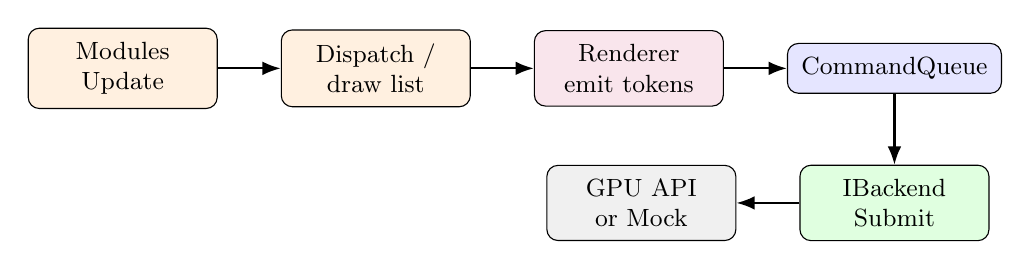
\begin{tikzpicture}[
  font=\small,
  box/.style={draw, rounded corners, align=center, inner sep=5pt, minimum width=2.4cm},
  arr/.style={-{Latex}, thick}
]
  \node[box, fill=orange!12] (mod) {Modules\\Update};
  \node[box, fill=orange!12, right=0.8cm of mod] (disp) {Dispatch /\\draw list};
  \node[box, fill=purple!10, right=0.8cm of disp] (ren) {Renderer\\emit tokens};
  \node[box, fill=blue!10, right=0.8cm of ren] (q) {CommandQueue};
  \node[box, fill=green!12, below=0.9cm of q] (be) {IBackend\\Submit};
  \node[box, fill=gray!12, left=0.8cm of be] (gpu) {GPU API\\or Mock};

  \draw[arr] (mod) -- (disp);
  \draw[arr] (disp) -- (ren);
  \draw[arr] (ren) -- (q);
  \draw[arr] (q) -- (be);
  \draw[arr] (be) -- (gpu);
\end{tikzpicture}
\end{center}

\subsection{Layering}

\begin{lstlisting}[language={}]
Game / Rulesets / UI
    |  (no gl* for draw submission)
    v
Drawable::AppendCommands(Renderer*)
    |  acquire/enroll typed handles + push tokens
    v
CommandQueue<RenderCommand>   // tagged union payloads
    |
    v
IBackend::SubmitCommandQueue
    |
    +-- GLBackend + GLDevice   (private production factory; one fallible init)
    +-- MockBackend            (Illumo::TestSupport)

Renderer.h depends only on IBackend*; OpenGL types stay under Rendering/OpenGL/.
\end{lstlisting}

\subsection{Drawable meaning}
``Drawable'' means \emph{something that can append tokens} (and optionally fall
back to immediate \texttt{Draw}). GL objects live in backend registries, not on
\symbolref{DrawableBase}.

CanvasView end state (shipped):
\begin{itemize}
  \item Domain: \texttt{SparseCellGrid}, signed coordinates, 16$\times$16
        chunks, retained candidate/frontier structures, and adaptive
        candidate-or-18$\times$18-halo stepping. Large candidate and halo work
        uses bounded reusable workers; discovery and transactional merge remain
        deterministic.
  \item View: revision-gated camera sampling + RGB fade buffers + one
        nearest-filtered RGB display texture and one world-space quad. The
        quad and editor cursor share 16$\times$16 cell bounds at normal zoom;
        far zoom uses a density overview at about four screen pixels per
        texel. Dirty-rect \texttt{UpdateTexture} remains the only texture
        upload (PBO) and idle frames do not resample or upload.
  \item See \pathref{docs/architecture-consensus.md} for the single canonical
        presentation model (R8-only notes are historical).
\end{itemize}

\subsection{Migration phases (historical checklist)}
\label{sec:migration-phases}

\begin{enumerate}[leftmargin=*]
  \item \textbf{Phase 0 --- Document \& freeze vocabulary} \quad \textbf{done}
  \item \textbf{Phase 1 --- Token proof path} \quad \textbf{done}
        (\texttt{RenderProofQuad}, tagged union, mesh upload, handle resolve)
  \item \textbf{Phase 2 --- Scene through Renderer} \quad \textbf{done}
  \item \textbf{Phase 3 --- Canvas tokens} \quad \textbf{done}
        (later: dirty-rect uploads; D-P4 R8 experiment then fade restore)
  \item \textbf{Phase 4 --- UI drawables} \quad \textbf{done}
        (GLString, CommandLine, SplashText)
  \item \textbf{Phase 5 --- Dead path cleanup} \quad \textbf{done}
        (archive under \pathref{archive/dead-render/}; pure DrawableBase)
  \item \textbf{Phase 6 --- Mock backend} \quad \textbf{done}
        (no second real API yet)
\end{enumerate}

\subsection{Acceptance criteria (migration ``done'')}
\begin{itemize}
  \item[\checkmark] Frame path is enroll + token queue + submit.
  \item[\checkmark] Cell sim runs: edit, step/rules, camera, console, FPS, splash.
  \item[\checkmark] \symbolref{Renderer::RenderScene} is non-empty and used.
  \item[\checkmark] Mock/headless tests cover tokens and domain.
  \item Partial: \texttt{gl*} still appears in window bootstrap and
        \pathref{Rendering/OpenGL/}; some non-Windows platforms lag.
\end{itemize}

\subsection{Optional future work}
\begin{itemize}
  \item Font atlases, UTF-8 layout, and nine-slice UI. General pixel clipping
        is shipped in D-R23.
  \item Chunked tilemaps, world-space sprite culling, and particle emitters.
  \item Multiple cameras, offscreen targets, compositing, and post-processing.
  \item The Illumo static library and supported public include tree are shipped;
        evolve that boundary only from concrete IllumoGame needs (D-E6).
  \item Second real graphics API (only if needed).
  \item GPU color fade without bringing back full-grid float RGB.
  \item Restore Linux/macOS bootstrap compatibility and validate those ports
        natively before changing their unsupported status.
\end{itemize}

\section{Services, foundation, platform}
\label{sec:services}

\subsection{Illumo services}
The library owns reusable cross-cutting facilities:
\begin{itemize}
  \item \textbf{Logging} --- \symbolref{Logger} with file/terminal sinks and a
        generic environment-controlled level.
  \item \textbf{Configuration} --- \symbolref{EnvVars}/\symbolref{IEnvVars}.
        The host supplies only generic window, presentation, logging, and console
        defaults. An explicit configuration path avoids working-directory
        dependence.
  \item \textbf{Input} --- \symbolref{InputManager}, \symbolref{InputContext},
        and \symbolref{KeyCode}; no Game types.
  \item \textbf{Console} --- parameterized \symbolref{CommandLine} branding,
        generic editing/history/alias/help behavior, generic host commands, and
        \symbolref{CommandRegistry} metadata/completion. Output entries carry a
        level, timestamp, and repeat count; view filters, scripts, log export,
        clipboard editing, reverse search, watched variables, and F-key
        bindings are generic console tools
        (D-UI4). The console draws with its own plain palette, not
        \texttt{UiTheme}.
  \item \textbf{System command line} --- \symbolref{SysCmdLine} owns
        help/version, window-dimension parsing, validation, and exit-code
        mechanics while accepting declarative application options.
  \item \textbf{Allocators} --- pool, arena, chain, and Debug allocation tools.
\end{itemize}

Arena and stack allocations align actual addresses. Empty backing storage may
gain stronger alignment; live allocations never move. New chunks and typed
pool storage honor over-aligned requests. The four-chunk cap, bulk clear and
stack LIFO behavior remain unchanged. Byte alignment zero means one; other
non-power-of-two alignments and overflowing sizes are rejected before use.
An underlying allocation failure ends the process (D-F3).

Command dispatch detaches one batch. Newly queued callbacks wait until the next
top-level dispatch; nested dispatch is ignored. Retiring or replacing a
registration cancels its unstarted callbacks. Clearing cancels pending work and
the detached remainder while preserving the active callback. Exceptions
propagate and discard the remainder, but dispatch can subsequently resume.
The registry and input manager are non-copyable and non-movable owners.

Configuration loads are transactional. Invalid or unreadable input disables
saving, including destruction-time saving, without overwriting the original
file. Repair or remove the file and successfully reload to restore persistence.
A missing file permits first-run creation. Failure diagnostics go through the
logger while it exists and fall back to standard error otherwise, so they do
not depend on logger lifetime.

Input callbacks retain at most 256 pending characters and 256 key events, counting
dropped new events. Release polling reports frame edges. Console execution and
public parsing preserve drive and UNC paths, quoted trailing separators, and
empty arguments. Console-owned command callbacks retire before destruction.
Logger retains a unique process instance with explicit runner shutdown and an
executable-adjacent default file; tests can select an explicit path. Each
session header records its start time and build, and file lines carry
wall-clock timestamps. Messages logged before the first console attaches are
kept (bounded, with an omitted count) and replayed into it once. Background
threads may log: file and terminal writes are serialized, while only the
owner thread forwards to the main-thread-affine console. Startup logs a build
and machine report from the platform \symbolref{SystemInfo} query, followed by
display, GPU, audio, package and guest-budget descriptions; subsystems log
lifecycle milestones at info and behind-the-scenes detail at trace.

\subsection{IllumoGame policy}
IllumoGame owns \pathref{CSim/envvars.json} and its CA defaults (canvas,
topology, ruleset, TPS, speed, and fade; \texttt{IllumoGameConfig::ApplyDefaults},
which its program applies once settings load). \symbolref{CanvasScene}
registers simulation, canvas, camera, ruleset, persistence, TPS, speed, and
fade commands while it is active. The Release-visible F1 settings surface (one
menu per scene, sharing \symbolref{SimulatorSettings}) updates the same product
variables. Generic Illumo services neither validate rulesets nor assume a game
program exists.

\subsection{Foundation}
Supported lightweight headers include macros, \pathref{MathTypes.h},
\pathref{ArrayQueue.h}, \pathref{RollingMetric.h}, and engine-owned
\pathref{BuildInfo.h}. Its values are defined by a source that
\pathref{cmake/IllumoVersion.cmake} regenerates on every build (D-F2): the
release from \pathref{VERSION.txt}, the first-parent commits since that file
last changed, the commit and a dirty flag, giving \texttt{v26.09\_12} for
display and \texttt{v26.09\_12 (1f709073, dirty)} for logs and
\texttt{--version}.

\begin{statusbox}
\pathref{MacroDefs.h} still pulls Windows headers on \texttt{\_WIN32} for
\texttt{Sleep}/\texttt{\_\_SLEEP}. D-F1 defers splitting that dependency until
measured include cost, collisions, or portability work justifies it.
\end{statusbox}

\subsection{Illumo platform boundary}
\pathref{Illumo/Source/Platform/} contains process entry and native persistence
dialogs behind the public \symbolref{SaveLoad} contract:
\begin{itemize}
  \item Windows \pathref{WinMain.cpp}/\pathref{WinSaveLoad.cpp} is supported.
  \item Linux sources target Ubuntu 24.04 x86\_64 X11/XWayland with gtkmm-3
        dialogs and clipboard; they are not supported until native smoke.
        The WASM runtime builds there only on request
        (\texttt{ILLUMO\_BUILD\_WASM\_RUNTIME=ON}, D-PL2), with its own
        module compiler helper
        (\pathref{Illumo/Source/Platform/Linux/LinuxWasmCompiler.cpp}).
        macOS is not targeted; its scaffold has been removed.
\end{itemize}
Platform bootstrap calls \symbolref{CreateIllumoApplication} and then the
engine-owned \symbolref{RunIllumoApplication}. Each platform implements the
engine-owned \symbolref{SaveLoad} contract; the game supplies only dialog text
and filename defaults through \symbolref{SaveLoadDialogSpec}. Source presence
and CMake selection do not establish support: a port still requires native
configure, build, launch, tests, rendering/input, dialogs, and shutdown
validation.

An engine-internal \texttt{PixelWindow} provides secondary GLFW windows
without a client API for CPU-drawn tools (the detached console, D-UI5). GLFW
handles creation, input, and native move/resize/close; a per-OS presenter blits
the image (Windows GDI; Linux reports it unsupported). No second OpenGL
context is created.

SaveLoad strings and returned paths use UTF-8. Windows adapts them to wide common
dialogs with a 32,768-character path buffer. Codecs convert UTF-8 paths explicitly
and contain encoding failures. CMake rejects Apple targets because no macOS
platform implementation is retained.

Product save codecs use \texttt{AtomicFile::write}: exclusively create a sibling
staging file, encode, check write/flush/close, then replace the destination.
Reported failures preserve prior bytes and clean only owned staging files.
Windows replacement uses \texttt{MoveFileExW} without cross-volume copy fallback;
POSIX \texttt{rename} replaces on the same filesystem and fails with
\texttt{EXDEV} across devices, with no copy fallback. Formats stay
product-owned and unchanged. This is not a power-loss durability guarantee.

The shared \texttt{.ilsc} format 2 parser (\texttt{IlscCodec} in
\texttt{Illumo::Content}) validates numeric destination ranges before
narrowing: float fields reject non-finite values and finite doubles outside the
float range; integer fields check their JSON type and range before conversion.
Version and color validation therefore cannot be bypassed by integer wrapping.
Parsing is transactional: rejected input leaves the destination document
untouched. Format 1 files are refused with an explicit message. Accepted float
values are written back with the shortest round-trip form of the stored
\texttt{float}, so encoding the same document twice is byte-identical.

Node identifiers are opaque strings of at most 128 bytes, unique within the
document; existing ids and parent references are preserved, including long
numeric-looking ids. New nodes take the first unused \texttt{n} plus decimal
counter from \texttt{SceneInstance::uniqueId}, checked against every existing
id. The node table is bounded (\texttt{SceneDocument::kMaximumNodes}), so the
search always ends.

\subsection{Packages and the virtual file tree (D-E20 to D-E23)}
\texttt{IllumoRuntime} launches a package, not a loose module:
\begin{itemize}
  \item \texttt{--app <name>} resolves \pathref{apps/<name>/} (a directory)
        or \pathref{apps/<name>.ilpk} beside the runtime; the game is the
        default. \texttt{--package <dir|file.ilpk>} runs any other package.
        The package must be of kind \texttt{app}; its \texttt{illumo.json}
        title names the window, and its module and worker \texttt{.wasm}
        bytes are read through the file tree.
  \item Every package in \pathref{packages/} beside the runtime (directories
        holding \texttt{illumo.json}, and \texttt{*.ilpk} files) is discovered
        in file-name order; unreadable packages and duplicate ids are skipped
        with warnings.
  \item \texttt{--mount <dir|file.ilpk>} (repeatable) mounts one more package;
        a missing path or an id already mounted refuses to start.
  \item \texttt{--project <dir>} mounts a loose directory writable at
        \texttt{/project}; a missing directory refuses to start.
        \texttt{--mount} and \texttt{--project} are rejected with
        \texttt{--game}.
\end{itemize}
\texttt{PackageMounts::mountAll} assembles the tree: \texttt{/engine} from the
runtime \pathref{Assets/} (or, in a distribution, \texttt{engine.ilpk}, which
the runtime also installs as the host's default asset source; D-E38),
\texttt{/app} from the launched package under the
overlays of every package that targets it (stacked by priority, dependency
order, then id), \texttt{/packages/<id>} for every package whose dependencies
resolve, and the optional \texttt{/project}. The mount table is an immutable
snapshot swapped under a mutex; open files keep their backend alive after an
unmount. Directory backends compare exact on-disk names, so lookups are
case-sensitive everywhere and a link that leaves the root does not resolve.
Writes reach only \texttt{/project}, through \texttt{AtomicFile}, and
\texttt{*.wasm} and \texttt{illumo.json} are refused there.

An application whose manifest sets \texttt{app.launchApps} is also offered the
\texttt{Project} capability in interactive runs (D-E42).
\texttt{GuestService::Project} lets it list recent projects, choose or create
one through the OS folder dialog (\texttt{SaveLoad::GetFolderLocation}),
clear the list, and open an entry: \symbolref{RuntimeProjectHost} keeps the
list as \texttt{recentProjects.<app>} in the runtime's settings, scaffolds a
new project, and on open records \texttt{--project <dir>} as the arguments
\texttt{RelaunchCurrentProcess} replays, so the guest's restart request
closes the window and starts the runtime again on the chosen folder. Only ids
and folder names cross the ABI.

The host console command \texttt{vfs} (registered beside \texttt{wasm\_stats}
when a tree exists) runs \texttt{VfsConsole}:
\texttt{vfs mounts}, \texttt{vfs ls <path>}, \texttt{vfs tree <path> [depth]}
(capped at 400 lines), \texttt{vfs stat <path>} (kind, size, supplying
package), and \texttt{vfs cat <path> [bytes]} (text, or a hex dump for binary
data, at most 64\,KiB). None of them prints a host path.

The host also publishes the tree to engine tools as the core, read-only
\symbolref{IFileTreeSource} \texttt{IllumoContext::fileTree}
(\texttt{VfsTreeSource}, at most 4,096 entries per listing). In debug-tools
builds, \symbolref{DebugOverlay}'s \texttt{files [path|off]} command opens a browser over
it (\texttt{FileTreeOverlay}, drawn with \texttt{GuiFileTree}). It is driven by
the keyboard and wheel only, and consumes that input before the product sees
it; the footer shows the selection's size and supplying package.

\subsection{Guest file protocol v2 (D-E23, D-E24)}
\texttt{GuestFileRequest} version 2 adds the \texttt{Mounted} area (absolute
virtual paths; \texttt{Package} remains an alias for \texttt{/app}) and the
actions \texttt{List} (a cursor and a page of at most 256 entries),
\texttt{Stat} (kind, size, package id), \texttt{Import} (copy a Selected grant
into \texttt{/project/<path>}), and \texttt{Pack} (\texttt{/project} into an
\texttt{.ilpk} at a writable Selected grant, on a dedicated host pack worker).
Version 1 requests are refused; the host and guest SDK ship together. Mounted
transfers use blocks up to 1\,MiB; Package, Storage and Selected files keep
64\,KiB. \texttt{GuestFiles} holds 16 tasks in flight.

Reading and listing mounted paths need the \texttt{Assets} capability. The new
\texttt{ProjectFiles} capability (bit 9; \texttt{KnownCapabilities} is
\texttt{(1 <{}< 10) - 1}) is offered only while \texttt{/project} is mounted;
project writes, Import and Pack need it, and Import and Pack also need
\texttt{SelectedFiles}. Project writes stage in memory and commit through the
file tree under an incrementally maintained quota
(\texttt{WasmFileLimits::projectBytes}). Pack requires a valid
\texttt{illumo.json} at the project root; a replace that fails, for example
because the target archive is mounted, reports \texttt{IoError}.

The guest SDK wraps this as \texttt{GuestFileTree} (list, stat, read, write,
import, pack with completion callbacks). \texttt{GuestVfsAssets} replaces
\texttt{GuestPackageAssets} as AssetManager's guest byte source: pinned
\texttt{packageAssets()} preloads, fetch sets held until released, a
least-recently-used byte budget (256\,MiB by default), and app-supplied bytes
under \texttt{/local/<name>}. \texttt{GuestSceneFetches} (in
\texttt{IllumoGuestContent}) fetches a scene's references, then the MTL
libraries its OBJ files declare, tolerating missing libraries.

\subsection{Text entry and file-tree helpers (D-UI6)}
\texttt{Illumo/Gui} gains two value-state helpers for native and guest code.
\texttt{GuiTextEdit} is single-line UTF-8 editing: caret and selection at
code-point boundaries, word jumps, a byte limit clipped at a code point, Enter
or Tab commit, Escape cancel, and clipboard hand-off (copy and cut return text;
paste raises a request the caller completes). While active it consumes the
key and character queues it reads (\texttt{InputManager::getCharQueue}), so
product shortcuts do not fire. \texttt{GuiKit::drawTextField} draws it.
\texttt{GuiFileTree} holds expansion state and the listings received so far,
names directories still to list (\texttt{takePendingListings}), and flattens
rows depth first with an explicit stack (directories first, at most 20,000
rows); \texttt{GuiKit::drawTreeRow} draws each row. Neither is a retained
widget tree.

\subsection{Engine brand (D-UI14)}
\texttt{GuiEngineBrand} draws the Illumo brand from images in
\path{Illumo/Assets/Branding}, which a guest reads as \texttt{/engine/Branding}.
Guest textures have no mipmaps, so \path{tools/make_brand_assets.py} crops the
kit's logos and pre-sizes them near the size they are drawn at.
\texttt{GuiEngineSplash} owns its two layers, its clock and its skip input, and
\texttt{RuntimeShell} plays it on every interactive launch
(section~\ref{sec:runtime} describes how it holds the program).
\texttt{GuiEngineBadge} holds only its image and draws a `Powered by'' label
over the flat wordmark into the caller's visual; every \texttt{GuestProgram}
preloads that image, and CSim's title screen draws the badge in its lower left
corner. A missing image ends the splash at once and leaves the badge undrawn.

\subsection{Plain tool look and detachable panels (D-UI7, D-E27)}
IllEd and IllMeshViewer draw with \texttt{GuiToolStyle}: a neutral palette in
the spirit of the console's, flat rectangles, lines and text, fixed tool
metrics and no animation. Their panels live in one \texttt{GuiPanelDock} per
app window, which stacks them in left and right columns with draggable
splitters and gives each a title bar that hides it or pops it out; dragging a
title past the window edge tears it off, and a detached panel docks back from
its title bar, its close box or View \textgreater{} Reset Layout. The dock
never draws content. Each panel draws into a \texttt{GuiPanelPlacement}
(content rectangle and surface) and reads its pointer through
\texttt{GuiPanelPointer}, which samples the main window or the panel's own
window and ignores presses the menu bar or dock chrome took. The layout is
saved in the \texttt{panelLayout} setting.

Extra windows come from \texttt{IllumoContext::panelSurfaces}
(\texttt{IPanelSurfaces}): surface 0 is the main window, other surfaces are
opened by id and report size, screen origin, pointer and window events, and
keys stay in the one input queue. Guests reach it through the
\texttt{Windows} capability; the host renders a changed surface offscreen,
reads it back asynchronously and presents it in a \texttt{GLFW\_NO\_API}
window one frame late (D-R27). Hosts without windows omit it, and every panel
stays docked.

\subsection{Sound effects and music (D-E28, D-E32)}
\texttt{IllumoContext::audio} (\texttt{IAudio}) plays sound effects and music:
a product registers a decoded \texttt{AudioClip} once and plays it by
\texttt{SoundHandle}, each play an independent voice with its own volume, pan
and pitch. A play may loop and fade in; \texttt{stop} ends one sound's voices,
optionally fading them out, and \texttt{setVolume} changes their gain, so a
music track can loop behind a screen and follow a volume setting. Looping
voices are the last replaced when every voice is busy.
\texttt{AudioDecoder} turns WAV, FLAC or MP3 bytes into float
samples at the source rate; \texttt{AudioDevice}, the native implementation,
mixes voices on the default output device and converts each to the device's
rate. Both wrap vendored miniaudio, which no public header exposes, and the
decoder reaches only miniaudio's memory entry points.

Guests decode their own package files and send the samples through the
\texttt{Audio} capability's service, so the host never parses a guest's
encoded audio. \texttt{GuestAudio} implements \texttt{IAudio} over that
service with guest-local handles; its requests complete at once and their
completions are discarded. A clip larger than one service record (a music
track) travels in chunks over several exchanges, held in order in a guest
backlog, and the host registers it when the last chunk lands. The runtime
opens one output device, except for captures and benchmarks, and releases a
guest's sounds when the guest retires. Without an output, \texttt{audio} is
null and products run silently. CSim's cues (\texttt{CSimSounds}) scale with
its \texttt{soundVolume} setting; its title screen loops the main-menu
music, and its canvas loops an edit track only while it is in EDIT, both at
the separate \texttt{musicVolume} setting.

\subsection{Third-party and runtime data}
Dependencies remain vendored under \pathref{Illumo/thirdparty/}. Illumo owns
its shaders, fonts, RendererDemo assets, notices, and dependency licenses and
provides the CMake staging helper. IllumoGame separately seeds its default
configuration. New dependencies still require the contributing-policy review.

\section{Design decision log}
\label{sec:decisions}

Append-only log. Newest entries at the bottom. If a decision is reversed, add a
new entry that supersedes the old id; do not silently delete history.

%----------------------------------------------------------------------------
\subsection*{D-001 --- Package rename (structure)}
\begin{decisionbox}[title={D-001 \quad 2026-07-28}]
\textbf{Decision:} Rename/split ambiguous folders to match responsibility:
\texttt{Core$\rightarrow$Game}, \texttt{System$\rightarrow$\{App,Engine,Services\}},
\texttt{Init+Util$\rightarrow$Foundation}, \texttt{AssetLoaders$\rightarrow$Assets}.\\
\textbf{Why:} Names were lying; slowed reasoning and migrations.\\
\textbf{Consequences:} Include/CMake paths updated; archive for old States.
\end{decisionbox}

%----------------------------------------------------------------------------
\subsection*{D-002 --- MathTypes header name}
\begin{decisionbox}[title={D-002 \quad 2026-07-28}]
\textbf{Decision:} Project math aliases live in \pathref{MathTypes.h}, not
\pathref{Math.h}.\\
\textbf{Why:} Windows case-insensitive include collision with CRT
\texttt{math.h}.\\
\textbf{Consequences:} All includes updated; the Foundation package map under
\pathref{docs/packages/} notes the trap.
\end{decisionbox}

%----------------------------------------------------------------------------
\subsection*{D-003 --- Render abstraction direction}
\begin{decisionbox}[title={D-003 \quad 2026-07-28 (implemented; see D-R*) }]
\textbf{Decision:} Command/token submission via \symbolref{IBackend}
+ \symbolref{RenderCommand} queue; game code must not permanently depend on
raw GL for draw submission.\\
\textbf{Why:} Multi-API optionality; clearer frame boundary; testability.\\
\textbf{Consequences:} Phases 1--6 complete for planned scope
(\cref{sec:migration-phases}); hybrid immediate \texttt{Draw} remains only as
fallback.
\end{decisionbox}

%----------------------------------------------------------------------------
\subsection*{D-004 --- Module frame hooks}
\begin{decisionbox}[title={D-004 \quad inferred from IModule}]
\textbf{Decision:} Modules expose \symbolref{Start}/\symbolref{Update}/
\symbolref{DispatchDrawables}/\symbolref{Exit}.\\
\textbf{Why:} Separate simulation tick from draw contribution.\\
\textbf{Consequences:} Draw list is rebuilt or contributed each frame through
dispatch. Module ownership/composition was later closed by D-E1.\\
\textbf{Status:} Superseded by D-E31. Program scenes keep the split
(\texttt{update} and \texttt{dispatch}) inside a program; the engine has no
modules.
\end{decisionbox}

%----------------------------------------------------------------------------
\subsection*{D-005 --- Rules as polymorphic sets}
\begin{decisionbox}[title={D-005 \quad inferred}]
\textbf{Decision:} Each CA variant is a \symbolref{RuleSet} subclass.\\
\textbf{Why:} Open for extension; shared generation sweep.\\
\textbf{Consequences:} Factory logic currently in \symbolref{CellContext}
string matching (could become a registry later).
\end{decisionbox}

%----------------------------------------------------------------------------
\subsection*{D-006 --- Mode handling (enum vs State classes)}
\begin{decisionbox}[title={D-006 \quad current code; author may supersede}]
\textbf{Decision (current):} \symbolref{CellState} enum inside
\symbolref{CellGameModule}.\\
\textbf{Supersedes:} class hierarchy under \pathref{archive/old-states/}.\\
\textbf{Why (inferred):} fewer types for a small mode set.\\
\textbf{Open at decision time:} SAVE/LOAD completeness; whether splash/global
state is acceptable.\\
\textbf{Resolution (2026-08-04):} frame modes are now
\texttt{NORMAL | EDIT | EXIT}; save/load are registered commands with validated
file handling (D-CLI1).
\end{decisionbox}

%----------------------------------------------------------------------------
\subsection*{D-007 --- Enrollment vs per-frame commands}
\begin{decisionbox}[title={D-007 \quad visible in Renderer comments}]
\textbf{Decision:} Resource creation goes through enroll/Create* APIs; do not
stuff mesh/shader creation into the per-frame token stream.\\
\textbf{Why:} Keep the frame queue about \emph{binding and drawing}.\\
\textbf{Consequences:} Need an explicit destroy/reload story for hot-reload
later.
\end{decisionbox}

%----------------------------------------------------------------------------
\subsection*{D-008 --- contributing constraints}
\begin{decisionbox}[title={D-008 \quad from docs/contributing.md}]
\textbf{Decision:} Avoid \texttt{auto}; avoid namespaces (prefer static
classes/structs); no recursion; third-party via PR.\\
\textbf{Why:} Author house style / learning constraints.\\
\textbf{Consequences:} Documentation and new code should respect these unless
explicitly waived in a later decision.
\end{decisionbox}

%----------------------------------------------------------------------------
\subsection*{D-R1 --- RenderCommand payload shape}
\begin{decisionbox}[title={D-R1 \quad 2026-07-28}]
\textbf{Decision:} \symbolref{RenderCommand} uses a \textbf{simple tagged union}
(\texttt{CommandType} + POD payload union), not a kitchen-sink flat struct and
not a byte-stream compiler. Prefer C-style union over \texttt{std::variant}.\\
\textbf{Why:} Type-safe uniforms/clear/update data while remaining
copyable for \symbolref{ArrayQueue}; matches house style.\\
\textbf{Consequences:} \pathref{Rendering/RenderCommand.h} redesigned; execute
path switches on type and reads the matching payload.
\end{decisionbox}

%----------------------------------------------------------------------------
\subsection*{D-R2 --- Who emits tokens}
\begin{decisionbox}[title={D-R2 \quad 2026-07-28}]
\textbf{Decision:} Each drawable emits its own tokens via
\texttt{AppendCommands(Renderer*)} (or equivalent). \symbolref{Renderer}
owns frame setup (clear/viewport) and submit.\\
\textbf{Why:} Smallest strangler step from today's
\symbolref{DispatchDrawables} list.\\
\textbf{Consequences:} Hybrid phase may still call immediate \texttt{Draw}
for unmigrated drawables after token submit.
\end{decisionbox}

%----------------------------------------------------------------------------
\subsection*{D-R3 --- Handle typing for v1}
\begin{decisionbox}[title={D-R3 \quad 2026-07-28}]
\textbf{Decision:} Keep \texttt{unsigned long} opaque handles with backend
registries (\texttt{tableID} $\rightarrow$ GL object). Strong typedefs deferred.\\
\textbf{Why:} Minimal churn; critical fix is resolve-on-submit, not type names.\\
\textbf{Consequences:} Execute must never treat handles as raw GLuints without
registry lookup.
\textbf{Status:} Historical v1 decision; superseded by D-R16.
\end{decisionbox}

%----------------------------------------------------------------------------
\subsection*{D-R4 --- Migration scope}
\begin{decisionbox}[title={D-R4 \quad 2026-07-28}]
\textbf{Decision:} Full migration Phases 1--5 (token proof $\rightarrow$ Scene
routing $\rightarrow$ Canvas $\rightarrow$ UI drawables $\rightarrow$ cleanup).
Phase 6 (mock backend) included; second real GPU API still optional.\\
\textbf{Why:} Playable strangler path to API isolation without big-bang rewrite.\\
\textbf{Also freeze for v1:} destroy resources at shutdown only; Windows GL is
primary platform. The lifetime clause is superseded by D-R16/D-R17.\\
\textbf{Superseded in part by D-P1/D-P4:} full-frame Canvas rewrite was v1 only.
Dirty-rect/PBO uploads remain, while the R8 presentation was later superseded
by the restored RGB fade path documented in D-P4.
\end{decisionbox}

%----------------------------------------------------------------------------
\subsection*{D-R5 --- Blend state on first enable}
\begin{decisionbox}[title={D-R5 \quad 2026-07-28}]
\textbf{Decision:} When enabling blending in \symbolref{GLDevice::ApplyPipelineState},
always call \texttt{glBlendFunc} (do not rely on CPU-side factor cache matching
defaults).\\
\textbf{Why:} OpenGL default is \texttt{ONE}/\texttt{ZERO}; cache defaults were
SrcAlpha/OneMinusSrcAlpha so factors looked ``unchanged'' and console panel
lost transparency after the token migration.\\
\textbf{Consequences:} Semi-transparent UI (console panel alpha) works again.
\end{decisionbox}

%----------------------------------------------------------------------------
\subsection*{D-R6 --- Dead stack cleanup (Phase 5)}
\begin{decisionbox}[title={D-R6 \quad 2026-07-28}]
\textbf{Decision:} Archive window \symbolref{RenderQueue}, legacy
\texttt{Drawable.cpp} GL helpers, empty \texttt{Transform}/\texttt{RenderContext},
and unused \texttt{CellCommandLine} under \pathref{archive/dead-render/}.
\symbolref{DrawableBase} is a pure list/token interface (no GL handles).\\
\textbf{Why:} Token path won; dual submission models confuse maintenance.\\
\textbf{Consequences:} \texttt{IRenderWindow::getRenderQueue} removed; frame
draw list is only \symbolref{Scene} + \symbolref{Renderer}.
\end{decisionbox}

%----------------------------------------------------------------------------
\subsection*{D-R7 --- Mock backend for tests (Phase 6)}
\begin{decisionbox}[title={D-R7 \quad 2026-07-28}]
\textbf{Decision:} Add headless \texttt{MockBackend} implementing
\symbolref{IBackend}: record \texttt{Create*} and snapshot the command queue
on \texttt{SubmitCommandQueue}. Originally shipped as CMake target
\texttt{IllumoRenderTests} / CTest \texttt{MockBackend}; the current library
runner is \texttt{IllumoTests}, with exact \texttt{Illumo.*} CTest cases. The
old target and single-test names are no longer retained. Do \textbf{not} add
Vulkan/Metal yet.\\
\textbf{Why:} First meaningful automated render test without a GPU context;
proves token vocabulary and handle plumbing independently of GL.\\
\textbf{Consequences:} Library tests use \texttt{Illumo::TestSupport}; workspace
CI aggregates the library and game runners under the \texttt{IllumoWorkspace}
label. A second graphics backend remains future work after production needs
appear.
\end{decisionbox}

%----------------------------------------------------------------------------
\subsection*{D-R8 --- Inject IBackend into Renderer}
\begin{decisionbox}[title={D-R8 \quad 2026-07-28, refined 2026-08-07}]
\textbf{Decision:} \symbolref{Renderer} is backend-neutral: its only constructor
takes an injected \symbolref{IBackend*} and a \texttt{takeOwnership} flag.
Production library initialization constructs the real backend via
\texttt{CreateOpenGLBackend} under \pathref{Rendering/OpenGL/}, initializes it
exactly once, and transfers a \texttt{std::unique\_ptr<IBackend>} into the
renderer. Tests inject \texttt{MockBackend} through the same ownership
boundary. \texttt{Renderer.h} must not include or construct concrete OpenGL
types.\\
\textbf{Why:} End-to-end drawable $\rightarrow$ enroll/token $\rightarrow$ submit
without a GPU; second platforms can supply a different \symbolref{IBackend}
without touching the generic frame-submit surface.\\
\textbf{Consequences:} \texttt{TestRendererE2E} covers inject, owned-backend
composition style, header neutrality, \texttt{RenderScene}, Canvas tokens,
hybrid immediate drawables, and \texttt{RenderProofQuad}. OpenGL sources stay
under \pathref{Rendering/OpenGL/}; Mock under \pathref{Rendering/Mock/}.
\end{decisionbox}

%----------------------------------------------------------------------------
\subsection*{D-P1 --- Dirty visual path}
\begin{decisionbox}[title={D-P1 \quad 2026-07-28}]
\textbf{Decision:} Canvas/CellGameModule use dirty flags so idle frames skip
full-grid visual work and GPU upload.\\
\textbf{Why:} Dominant cost was recoloring + full texture upload every render
frame even when the CA did not step.\\
\textbf{Consequences:} \texttt{cellsDirty}, upload pending, early-out
\texttt{tickVisual}; still life after sim step does not re-dirty.
\end{decisionbox}

%----------------------------------------------------------------------------
\subsection*{D-P2 --- UI batching and geometry cache}
\begin{decisionbox}[title={D-P2 \quad 2026-07-28}]
\textbf{Decision:} CommandLine emits one packed \texttt{UpdateBuffer}/draw when
open and dirty; GLString caches GPU geometry until content/style changes.
Settled CommandLine frames keep one \texttt{DrawIndexed} and skip the buffer
upload.\\
\textbf{Why:} Per-line uploads and FPS string rebuilds were measurable when the
console/FPS overlay was active. Re-wrapping the full history and baking a
per-frame accent pulse kept the open console expensive.\\
\textbf{Consequences:} Token stream stays small; FPS may rebuild $\sim$1\,Hz;
idle console history reuses the last mesh until scroll, input, layout, caret
phase, or a quantized pulse changes.
\end{decisionbox}

%----------------------------------------------------------------------------
\subsection*{D-P3 --- Double-buffer CA generation}
\begin{decisionbox}[title={D-P3 \quad 2026-07-28}]
\textbf{Decision:} \texttt{RuleSet::calcGeneration} writes pure
\texttt{nextState(cell, aliveNeighbors)} into a scratch buffer, then
\texttt{memcpy}s back; neighbor counts use raw grid pointers + toroidal wrap.\\
\textbf{Why:} Correct simultaneous update; faster than per-cell
\texttt{getCanvasPixel}/in-place virtual writes; sparse dirty AABB for visuals.\\
\textbf{Consequences:} All active rulesets override \texttt{nextState}; stubs
use identity.\\
\textbf{Refined by D-P5 (2026-08-06):} scratch lives on \symbolref{CellGrid}
as a back buffer; promotion is pointer swap, not full-grid \texttt{memcpy}.
\end{decisionbox}

%----------------------------------------------------------------------------
\subsection*{D-P5 --- Single-pass dirty AABB + buffer swap}
\begin{decisionbox}[title={D-P5 \quad 2026-08-06}]
\textbf{Decision:} Track changed-cell AABB during the eval pass; store next
generation in \texttt{CellGrid} back buffer; on any change call
\texttt{swapLifeBuffers()} and mark the sparse dirty region. Interior Moore
counts skip toroidal wrap branches.\\
\textbf{Why:} Second full-grid compare pass and full \texttt{memcpy} write-back
dominated serial generation cost on large dense grids.\\
\textbf{Consequences:} \texttt{lifeCanvas} always means current front; rules
must not retain raw pointers across a swap; still life leaves domain clean.
\end{decisionbox}

%----------------------------------------------------------------------------
\subsection*{D-P6 --- Fade loop + packed dirty PBO staging}
\begin{decisionbox}[title={D-P6 \quad 2026-08-06}]
\textbf{Decision:} Keep CPU RGB fade presentation. Hoist coordinates in
\texttt{tickVisual}/\texttt{snapVisualToTargets}; rectangular target rebuild
uses one \texttt{includeRect}. \texttt{GLTexture::UpdateSubImage} packs partial
dirty rects tightly and maps only the staging range (no full-buffer orphan
every frame).\\
\textbf{Why:} Per-cell div/mod and full-texture PBO orphan were measurable on
large dirty rects while fade quality must stay.\\
\textbf{Consequences:} Fade math unchanged; MockBackend token path unaffected.
\end{decisionbox}

%----------------------------------------------------------------------------
\subsection*{D-P7 --- Optional row-parallel generation}
\begin{decisionbox}[title={D-P7 \quad 2026-08-06}]
\textbf{Decision:} \texttt{RuleSet::calcGeneration} may partition rows across
workers when cell count $\ge 512\times 512$ (auto) or when
\texttt{setWorkerOverride(N)} forces $N$ workers. Results are bit-identical to
serial. Presentation/fade stays main-thread.\\
\textbf{Why:} Large dense grids are eval-bound after D-P5; spawn cost makes
parallel unhelpful on default $80\times 60$.\\
\textbf{Consequences:} Tests cover serial/parallel identity
(\texttt{IllumoGame.Sim.SerialParallelIdentical}); micro-benches under
\texttt{IllumoGame.Sim.MicroBench}. Persistent thread pool deferred.
\end{decisionbox}

%----------------------------------------------------------------------------
\subsection*{D-P4 --- dirty-rect PBO uploads (R8 path partially superseded)}
\begin{decisionbox}[title={D-P4 \quad 2026-07-28}]
\textbf{Decision (original):} Present cells as \texttt{GL\_R8} texture of state
bytes plus a $256\times 1$ RGB palette (\texttt{evalCell}). Upload dirty rects
via PBO ping-pong in \texttt{GLTexture::UpdateSubImage}. Drop dual float RGB
staging.\\
\textbf{Why:} Large grids: bandwidth and CPU of RGB float fade dominated.\\
\textbf{Consequences (kept):} dirty-rect \texttt{UpdateTexture}, PBO path,
bind-state tracker in \symbolref{GLDevice}.\\
\textbf{Superseded presentation (2026-07-30):} live path restored to CPU RGB
fade (\texttt{targetRgb}/\texttt{displayRgb}) + RGB display texture so cell
colors ease rather than snap. R8+palette is historical experiment, not current
code truth. Canonical: \pathref{docs/architecture-consensus.md}.
\end{decisionbox}

%----------------------------------------------------------------------------
\subsection*{D-E1 --- Module registration lives in App}
\begin{decisionbox}[title={D-E1 \quad 2026-07-28}]
\textbf{Decision:} \symbolref{Illumo} does not include or construct
\symbolref{CellGameModule}. Today,
\pathref{IllumoGame/Source/App/CellMain.cpp} applies product configuration,
calls fallible \texttt{initialize}, then registers the required game module and
the optional Debug module before \texttt{startModules}.\\
\textbf{Why:} Engine must not depend on Game headers; product composition
belongs at the application boundary.\\
\textbf{Consequences:} New products/tests can register different module sets;
Engine only knows \symbolref{IModule}.\\
\textbf{Status:} Superseded by D-E31. The engine still never includes product
code, but there is nothing to register: IllumoRuntime runs one WASM program.
\end{decisionbox}

%----------------------------------------------------------------------------
\subsection*{D-E2 --- InputManager has no Game types}
\begin{decisionbox}[title={D-E2 \quad 2026-07-28}]
\textbf{Decision:} Remove \texttt{CellContext*} and Game includes from
\symbolref{InputManager}. Also drop unused \texttt{SplashText} extern from the
input header.\\
\textbf{Why:} Services must not depend on Game; input is a pure device/action
service. Splash and rules stay in Game/Rendering.\\
\textbf{Consequences:} InputManager header only needs KeyCode/InputContext/GLFW.
\end{decisionbox}

%----------------------------------------------------------------------------
\subsection*{D-E3 --- EntityTable is not the cell path}
\begin{decisionbox}[title={D-E3 \quad 2026-07-28}]
\textbf{Decision:} Archive \pathref{EntityTable.h} and \pathref{ModuleObject.h}
under \pathref{archive/dead-engine/}. Remove \texttt{entityTable} from
\symbolref{Scene}/\symbolref{IllumoContext}.\\
\textbf{Why:} Nothing allocated or used an EntityTable; the live path is
drawables + tokens, not ECS.\\
\textbf{Consequences:} Reintroduce a general object table only when a real
feature needs it; document that cells are not entities.
\end{decisionbox}

%----------------------------------------------------------------------------
\subsection*{D-E4 --- Scene is a drawable list, not a graph}
\begin{decisionbox}[title={D-E4 \quad 2026-07-28}]
\textbf{Decision:} \symbolref{Scene} holds only \texttt{drawables},
\texttt{window}, and \texttt{activeCamera}. Remove \texttt{root},
\texttt{nodeLookup}, no-op \texttt{Update}, and unused
\texttt{RenderableObject}. Archive \pathref{SceneObject.h}; \symbolref{Camera}
and \symbolref{CommandLine} no longer inherit a node graph.\\
\textbf{Why:} Architecture review (dead graph scaffolding); production never
used parent/child transforms for cells or UI.\\
\textbf{Consequences:} Frame contribution model is explicit and small.\\
\textbf{Status:} Refined by D-E31: the type is now \texttt{DrawList}
(\pathref{Illumo/Include/Illumo/Rendering/DrawList.h}).
\end{decisionbox}

%----------------------------------------------------------------------------
\subsection*{D-E5 --- Freeze IllumoContext; validate at Start}
\begin{decisionbox}[title={D-E5 \quad 2026-07-28}]
\textbf{Decision:} Keep \symbolref{IllumoContext} as a service bag for the
\textbf{two shipped modules} only. Document required fields per module.
\texttt{Start()} logs an error and bails if the bag is incomplete.
Do not grow the bag for convenience; a third module should take explicit
constructor dependencies if its subset differs.\\
\textbf{Why:} Architecture review --- bag cost is zero at $N=2$ but becomes a
de-facto global API as $N$ grows.\\
\textbf{Consequences:} \texttt{IllumoContextHasGameCore} /
\texttt{IllumoContextHasDebugCore} helpers; freeze note on the struct.\\
\textbf{Status:} Refined by D-E31. The bag stays frozen, minus
\texttt{moduleHost} and plus \texttt{scenes}; the program, each scene's
\texttt{start} and \texttt{DebugOverlay::start} check what they need.
\end{decisionbox}

%----------------------------------------------------------------------------
\subsection*{D-C1 --- Canvas dual role is intentional (for now)}
\begin{decisionbox}[title={D-C1 \quad 2026-07-28}]
\textbf{Decision:} Keep \symbolref{Canvas} as domain grid + fade view + GPU
enroll in one type. Document the scale wall: full-grid
\texttt{calcGeneration}, dual float RGB buffers ($\sim$24\,B/cell), no
chunked simulation domain.\\
\textbf{Why:} Locality for dirty-rect + palette + fade; headless tests already
use injected MockBackend rather than pure LifeGrid.\\
\textbf{Consequences:} Split \texttt{LifeGrid}/\texttt{CanvasView} only if pure
sim tests or large canvases become product requirements.
\end{decisionbox}

%----------------------------------------------------------------------------
\subsection*{D-R9 --- String-named uniforms are backend debt}
\begin{decisionbox}[title={D-R9 \quad 2026-07-28}]
\textbf{Decision:} Keep \texttt{char name[32]} uniforms for OpenGL + Mock.
Treat as debt if a second \emph{real} GPU backend is adopted; prefer binding
points / pre-resolved locations then.\\
\textbf{Why:} Architecture review --- uniform path is the least portable part
of \symbolref{RenderCommand}; handles and UpdateTexture are closer to neutral.\\
\textbf{Consequences:} Comment on uniform payloads; no API change now.
\end{decisionbox}

%----------------------------------------------------------------------------
\subsection*{D-R10 --- Production drawables are pure-token}
\begin{decisionbox}[title={D-R10 \quad 2026-07-28}]
\textbf{Decision:} \symbolref{Canvas}, \symbolref{CommandLine},
\symbolref{GLString}, \symbolref{SplashText} use
\texttt{AppendCommands} only (return true when contributing). Immediate
\texttt{Draw()} hybrid remains for tests/stubs. CRTP \texttt{DrawImpl} is
legacy for that fallback.\\
\textbf{Why:} Migration complete for shipped UI/canvas; dual path is debt only
where unmigrated types exist.\\
\textbf{Consequences:} Documented in \pathref{Drawable.h} and
\texttt{Renderer::RenderScene}.
\end{decisionbox}

%----------------------------------------------------------------------------
\subsection*{D-R14 --- Scene layers and built-in render styles}
\begin{decisionbox}[title={D-R14 \quad 2026-08-07}]
\textbf{Decision:} Introduce \textbf{Phase A} composition without multi-pass
GPU targets:
\begin{itemize}
  \item \symbolref{Scene} buckets drawables into ordered layers
        (\texttt{World}, \texttt{UI}, \texttt{Debug}) within one main pass
        (default framebuffer, single clear).
  \item \symbolref{Renderer} owns built-in \symbolref{RenderStyle} entries
        (\texttt{Canvas}, \texttt{UiText}, \texttt{Console}): each holds a
        shader table handle plus \texttt{PipelineState} defaults.
  \item Production drawables keep content handles (mesh/texture/domain data)
        and call \texttt{bindStyle} before content tokens.
\end{itemize}
Layers are not GPU target/load-store passes. Unimplemented pass scaffolding is
removed; explicit offscreen targets remain deferred.\\
\textbf{Why:} World/UI/debug stacking and shared draw policy should not live
as duplicated per-drawable shader enrollment and ad-hoc pipeline structs.\\
\textbf{Consequences:} \pathref{RenderLayerId.h}, \pathref{RenderStyle.h},
\pathref{RendererStyles.cpp}; modules pass a layer to
\texttt{Scene::AddDrawable}; docs distinguish layer vs pass.
\end{decisionbox}

%----------------------------------------------------------------------------
\subsection*{D-R15 --- Render primitives and GameVisual host}
\begin{decisionbox}[title={D-R15 \quad 2026-08-07}]
\textbf{Decision:} Introduce value-type \textbf{render primitives}
(\symbolref{ShapePrimitive}, \symbolref{SpritePrimitive}) composed on a
\symbolref{GameVisual} \texttt{Drawable} host.
\begin{itemize}
  \item Primitives are not Scene entries; the host is.
  \item Game/editor objects \textbf{embed} \symbolref{GameVisual} (or multiple)
        and add primitives to build complex visuals without hand-rolling
        enroll/bind/draw tokens.
  \item Built-in styles \texttt{Shape} and \texttt{Sprite} live on
        \symbolref{Renderer}; GPU mesh/texture/shader objects stay in the
        backend registries.
  \item Coordinate space is host policy (\texttt{Pixels} or \texttt{World}).
\end{itemize}
\textbf{Why:} Composition over per-primitive drawables keeps Scene traffic low
and matches D-R14 style ownership.\\
\textbf{Consequences:} \pathref{Rendering/Primitives/}; headless tests
\texttt{Illumo.GameVisual.*}; Canvas/UI paths unchanged.
\end{decisionbox}

%----------------------------------------------------------------------------
\subsection*{D-R16 --- Typed resource lifetime and bounded command growth}
\begin{decisionbox}[title={D-R16 \quad 2026-08-09}]
\textbf{Decision:} Replace raw renderer IDs with non-convertible
\texttt{MeshHandle}, \texttt{ShaderHandle}, \texttt{TextureHandle}, and
\texttt{RenderStyleHandle} values containing slot and generation. Backends
allocate handles and validate replace, destroy, validity, metadata, and command
resolution. Stale operations warn and safely no-op. Replace the fixed token
array with vector storage that reserves 2,048, grows as needed, and rejects only
at a configurable 65,536 default ceiling while reporting high-water and
rejection counts. Scissor state is explicitly enabled or disabled.\\
\textbf{Why:} Reusable rendering needs safe lifetime, hot replacement, and
realistic frame growth without silent corruption or unbounded memory.\\
\textbf{Consequences:} D-R3 and the fixed-capacity part of D-R12 are
superseded. Unimplemented command/pass scaffolding is removed. OpenGL and Mock
implement the same lifecycle contract.
\end{decisionbox}

%----------------------------------------------------------------------------
\subsection*{D-R17 --- Managed texture and shader assets}
\begin{decisionbox}[title={D-R17 \quad 2026-08-09}]
\textbf{Decision:} \symbolref{AssetManager} caches file textures by canonical
path plus options and shaders by canonical path pair. Duplicate acquisition
increments a reference count; final release destroys the backend resource.
Async is default, synchronous loading is available for startup/tests, one owned
worker performs file read/decode, and render-thread \texttt{pump} performs GPU
replacement. Stable fallbacks cover pending/failed initial loads. Failed reload
keeps the last good object. Debug polls timestamps every 500\,ms; all builds
retain explicit reload.\\
\textbf{Why:} Future 2D projects need deterministic resource ownership and live
iteration without compiling or mutating GPU objects from a worker.\\
\textbf{Consequences:} Managed scope is textures and shaders only. Dynamic quad
meshes stay renderer-owned; font atlases, model import, and general 3D meshes
remain outside this milestone.
\end{decisionbox}

%----------------------------------------------------------------------------
\subsection*{D-R18 --- Painter-correct 2D primitive stream}
\begin{decisionbox}[title={D-R18 \quad 2026-08-09}]
\textbf{Decision:} Give \symbolref{GameVisual} one stable ordered stream across
shape, sprite, and text values. Integer draw order is followed by insertion
sequence; only adjacent compatible items batch. Parent/local
\texttt{Transform2D}, normalized pivots, atlas regions, flips, and centered
sprite helpers are supported without a hierarchy. Dynamic quad buffers begin at
1,024, double, and stop at a configurable 65,536 default ceiling.
\symbolref{SpriteAnimator} is caller-updated and exposes only current visual
state with Once, Loop, and PingPong modes.\\
\textbf{Why:} Global texture sorting breaks overlapping alpha composition, and
animation time inside submission makes rendering nondeterministic.\\
\textbf{Consequences:} Top-left behavior remains the default $(0,0)$ pivot;
rendering observes state and never owns gameplay time.
\end{decisionbox}

%----------------------------------------------------------------------------
\subsection*{D-R19 --- Product proof before renderer extraction}
\begin{decisionbox}[title={D-R19 \quad 2026-08-09}]
\textbf{Decision:} Illumo is a cellular-automata application with a reusable 2D
renderer, not a general engine. A Debug-only first-party atlas and managed
sprite-shader showcase plus
\texttt{renderer\_demo}/\texttt{assets}/\texttt{asset\_reload} commands prove
the foundation in the product. Extract a standalone library only when a second
real project proves the required public boundary.\\
\textbf{Why:} A real consumer reveals the useful boundary better than detached
ECS, scene-graph, render-graph, or multi-backend scaffolding.\\
\textbf{Consequences:} Release composition remains unchanged. Follow-on work is
font/UI layout, tilemaps/culling/particles, then offscreen composition as actual
projects require.\\
\textbf{Status:} Superseded by D-E6. The approved consumer is the repository's
\texttt{IllumoGame} product, so the extraction records an explicit product
boundary; it is not evidence of a second independent product and does not
authorize speculative general-engine work.
\end{decisionbox}

%----------------------------------------------------------------------------
\subsection*{D-R20 --- Primitive-composed product UI}
\begin{decisionbox}[title={D-R20 \quad 2026-08-09}]
\textbf{Decision:} Build Illumo's existing UI drawables from
\symbolref{GameVisual} shape and text primitives. Keep
\symbolref{CommandLine} as the owner of console layout and interaction, retain
\symbolref{GLString}'s geometry cache while allowing optional panel chrome, and
use that decorated-label path for Debug FPS and fading EDIT/NORMAL notices.
Share colors and compact panel metrics through value-only \texttt{UiTheme}; do
not introduce a retained widget tree, layout engine, or additional render pass.\\
\textbf{Why:} The renderer foundation should prove useful composition in the
real product, and the console, FPS, and mode notice need one coherent visual
language without increasing Scene traffic or creating a second UI architecture.\\
\textbf{Consequences:} Console chrome now uses fills, outline rectangles, and
line primitives instead of a bespoke packed-quad aesthetic. Decorated labels
compose shadow, surface, border, accent, and text in one adjacent batch. Existing
editing, floating-window, fading, Scene-layer, and Debug/Release ownership
boundaries remain unchanged; headless tests assert the primitive composition.
\end{decisionbox}

%----------------------------------------------------------------------------
\subsection*{D-F1 --- MacroDefs Windows include deferred}
\begin{decisionbox}[title={D-F1 \quad 2026-07-30}]
\textbf{Decision:} Do \textbf{not} split \pathref{MacroDefs.h} /
\texttt{Windows.h} now. Revisit only if include toxicity causes real pain
(compile time, macro collisions, portability friction).\\
\textbf{Why:} Author priority --- convenience of \texttt{\_\_SLEEP} outweighs
hygiene until symptoms appear.\\
\textbf{Consequences:} Status note in services/platform section; not an open
blocker.
\end{decisionbox}

%----------------------------------------------------------------------------
\subsection*{D-N1 --- Illumo is the project and product name}
\begin{decisionbox}[title={D-N1 \quad 2026-08-04}]
\textbf{Decision:} Adopt \textbf{Illumo} as the repository-facing project,
product, CMake target, runtime title, console name, and save-format name. Keep
the existing \symbolref{Illumo} runtime-host class; the shared name is
intentional. Canonical tests are \texttt{IllumoTests}, and new saves use the
\texttt{.illumo} extension.\\
\textbf{Why:} The author selected Illumo as the permanent product identity.\\
\textbf{Consequences:} Live first-party source and documentation use Illumo;
generated build trees, vendored material, and archived historical artifacts are
not implementation sources and are not rewritten by this decision.\\
\textbf{Status:} Superseded by D-N2 and D-N4 for executable, product-visible,
test, and new-save filename identity. The Illumo repository/library/host name
and legacy \texttt{.illumo} loading remain valid.
\end{decisionbox}

%----------------------------------------------------------------------------
\subsection*{D-B1 --- DebugModule is excluded from Release}
\begin{decisionbox}[title={D-B1 \quad 2026-08-04}]
\textbf{Decision:} \symbolref{DebugModule} is Debug-build product composition
only. \symbolref{CellMain} must include/register it behind
\texttt{\#ifndef NDEBUG}, and CMake must compile its implementation only for the
Debug configuration.\\
\textbf{Why:} The developer overlay, console input handling, FPS/debug labels,
and instrumentation are development tools, not Release product behavior.\\
\textbf{Consequences:} Shared command/logging service code may remain available
to tests or non-UI systems, but Release must contain no DebugModule object or
module registration. Audit this boundary after CMake/composition changes.\\
\textbf{Status:} Still in force. Since D-E31 the overlay is
\texttt{DebugOverlay}, which \texttt{RuntimeShell} creates only in debug-tool
builds.
\end{decisionbox}

%----------------------------------------------------------------------------
\subsection*{D-CLI1 --- Split generic and domain console ownership}
\begin{decisionbox}[title={D-CLI1 \quad 2026-08-04}]
\textbf{Decision:} \symbolref{CommandLine} owns editing, parsing, help,
environment/application commands, and rendering. Product modules register
domain behavior through \symbolref{CommandRegistry}; each registration carries
usage, description, and optional completion candidates.\\
\textbf{Why:} Services should not acquire Game dependencies, while help and
completion must describe the commands that actually exist.\\
\textbf{Consequences:} \symbolref{CellGameModule} owns simulation, canvas,
ruleset, camera, and save/load commands. The shared known-ruleset list drives
validation/completion. Queued commands return successfully without falling
through to environment lookup or an unknown-command error.
\end{decisionbox}

%----------------------------------------------------------------------------
\subsection*{D-UI1 --- Measured console editor in one bounded batch}
\begin{decisionbox}[title={D-UI1 \quad 2026-08-04}]
\textbf{Decision:} Render the command caret and selection from measured text
prefixes, keep long input visible through a horizontal viewport, and retain one
batched token draw for console chrome and text. Size the dynamic mesh for 6,000
UI quads and regression-test a detailed help page beyond the former cap.\\
\textbf{Why:} An appended underscore produced an apparent cursor offset, while
the 2,000-quad mesh silently truncated easy-font output because each character
uses several quads.\\
\textbf{Consequences:} Editing supports selection and word operations without
lying about insertion position; a full help page remains one draw without
cutting off its final line.
\end{decisionbox}

%----------------------------------------------------------------------------
\subsection*{D-UI2 --- Wrapped console history with unified scroll metrics}
\begin{decisionbox}[title={D-UI2 \quad 2026-08-06}]
\textbf{Decision:} Word-wrap console history to the panel width, scroll by
visual lines rather than raw history entries, and compute PageUp/wheel/scrollbar
limits from the same floating-aware panel layout used when drawing. Raise the
console UI mesh to 8,000 quads to leave headroom for wrapped lines plus chrome.\\
\textbf{Why:} Hard truncation hid the rest of long help lines, and scroll
handlers used a mounted-only height estimate that disagreed with the floating
panel, so paging to the oldest history could leave text clipped or unreachable.\\
\textbf{Consequences:} Scrolling fully to the start of history shows the oldest
characters completely; floating resize and mounted mode share one max-scroll
definition; wrap metrics are cached until history or panel width change and
must stay equivalent to direct wrapping; a focused wrap/scroll regression
covers the clamp and batch path.
\end{decisionbox}

%----------------------------------------------------------------------------
\subsection*{D-DOC1 --- One first-party documentation tree}
\begin{decisionbox}[title={D-DOC1 \quad 2026-08-04}]
\textbf{Decision:} Keep all first-party project documentation under
\pathref{docs/}: current Markdown at the top level, package maps in
\pathref{packages/}, dated records in \pathref{sessions/}, provenance in
\pathref{history/}, one current LaTeX entrypoint at \pathref{latex/illumo.tex},
and generated output in \pathref{output/}.\\
\textbf{Why:} Competing LaTeX entrypoints and package READMEs scattered beside
code made current truth and PDF generation difficult to discover.\\
\textbf{Consequences:} The repository root keeps only the landing README and
AGENTS bootstrap as intentional prose exceptions. Licenses and vendored notes
remain beside governed assets. Architecture changes update Markdown, relevant
LaTeX chapters, and this append-only log together. \pathref{docs/build.ps1}
is the PDF wrapper and the optional default-build \texttt{IllumoDocs} target
uses that same script when TeX is available.
\end{decisionbox}

%----------------------------------------------------------------------------
\subsection*{D-T1 --- Granular CTest registration and coverage gate}
\begin{decisionbox}[title={D-T1 \quad 2026-08-04}]
\textbf{Decision:} Keep two compile-efficient runners: \texttt{IllumoTests}
for the reusable library and \texttt{IllumoGameTests} for product behavior.
Register each logical behavior as an exact owner-prefixed
\texttt{Illumo.<area>.<case>} or \texttt{IllumoGame.<area>.<case>} CTest entry.
CTest runs one filtered case per process in an isolated working directory and
aggregates both inventories under \texttt{IllumoWorkspace}. With
\texttt{ILLUMO\_ENABLE\_COVERAGE=ON}, Clang/LLVM adds the
\texttt{IllumoCoverage} target and enforces at least 85\% line coverage over
headless-testable first-party production code.\\
\textbf{Why:} A monolithic CTest result hid which of dozens of behaviors ran or
failed, and a narrow denominator could report a strong percentage while omitting
game commands, persistence, input, or assets.\\
\textbf{Consequences:} New behaviors receive separate stable names; file-backed
tests may run in parallel without sharing working files; combined coverage
merges both runners. Tests, vendored/system code, TestSupport, and the live
OpenGL backend are excluded from the automated production denominator. Native
dialogs, real-window behavior, and live OpenGL still require proportional smoke
tests. This supersedes the single-CTest-name registration detail in D-R7
without changing the MockBackend decision.
\end{decisionbox}

%----------------------------------------------------------------------------
\subsection*{D-UI3 --- Floating mode, title-bar dragging, and corner resize}
\begin{decisionbox}[title={D-UI3 \quad 2026-08-06}]
\textbf{Decision:} Extend \symbolref{CommandLine} to support dynamic window modes and resizable floating window geometry. Mode switching is driven by double-clicking the console title bar or executing \texttt{console\_mode [floating|mounted|toggle]}. In floating mode, left-clicking and dragging the title bar repositions the window across the screen, and dragging the bottom-right corner grip handle (or running \texttt{console\_size <W> <H> | reset}) resizes the console window dynamically with real-time viewport clipping and single-batch quad rendering.\\
\textbf{Why:} Enhances Developer Console usability, allows moving and scaling the console UI away from active grid regions, and provides modular window layout flexibility.\\
\textbf{Consequences:} \symbolref{CommandLine} geometry (chrome, history text, input trough, scrollbar, ghost text, selection highlight) is computed relative to dynamic floating bounds \texttt{panelX0}, \texttt{panelX1}, \texttt{panelY0}, \texttt{panelY1}; mouse press/drag event dispatch accounts for floating position offset and corner resize bounds.
\end{decisionbox}

%----------------------------------------------------------------------------
\subsection*{D-UI4 --- Plain developer console with levelled, filterable output}
\begin{decisionbox}[title={D-UI4 \quad 2026-09-23}]
\textbf{Decision:} The developer console stops using the product
\texttt{UiTheme} and draws with its own flat terminal palette: an opaque dark
panel, one-pixel border and rules, a header, an output band anchored at the
input, an input line, and a status bar (FPS/frame time, line counts, active
filters, scroll position, contextual hint). No full-screen shade, drop shadow,
pulsing accent, or panel easing remain; only the open/close slide animates.
Output entries record a \texttt{ConsoleLevel}, a timestamp, and a repeat count
(identical consecutive lines collapse). The buffer holds 2,048 entries;
command recall keeps 256. New built-ins: \texttt{filter}, \texttt{loglevel},
\texttt{timestamps}, \texttt{copy}, \texttt{savelog}, \texttt{exec},
\texttt{bind}/\texttt{unbind} (F1--F12 except host-reserved F3, F5, F6, F11),
\texttt{!!}/\texttt{!n}/\texttt{!prefix} recall, and \texttt{help <word>}
search; a follow-up added Ctrl+R reverse search, \texttt{add},
\texttt{cycle}, \texttt{watch}/\texttt{unwatch} (a live strip of up to eight
variables), \texttt{writeconfig}, click-to-recall on echoed commands,
severity marks, filter-match highlights, and a closed-console error/warning
badge (\texttt{alerts}). Clipboard and file access go through
\symbolref{CommandLineCore} virtual hooks and are compiled out of WASM
guests.\\
\textbf{Why:} The console is a debugging tool; styling it like the product
menus blurred that line, and a debugging session needs severity filtering,
repeat collapsing, scripts, and log export more than decoration.\\
\textbf{Consequences:} Hidden entries wrap to zero lines, so D-UI2 scroll
metrics and D-P2 settled replay are unchanged; a scrolled-back view stays
anchored while output arrives. Log prefixes (\texttt{ERROR:} and so on) stay
in entry text for compatibility. Guest console bridges forward collapsed
repeats and restore the success level on the host.\\
\textbf{Supersedes:} the console part of D-R20 (UiTheme styling)
\end{decisionbox}

%----------------------------------------------------------------------------
\subsection*{D-UI5 --- Detached console window without a second GL context}
\begin{decisionbox}[title={D-UI5 \quad 2026-09-23}]
\textbf{Decision:} The developer console can pop out into its own OS window
(header \texttt{pop out} button, \texttt{console\_mode detached}, or dragging
the floating title bar past the game window's edge) and return (\texttt{dock}
button, closing the window, or the console key from either window). The
window is
a GLFW \texttt{GLFW\_NO\_API} window owned by \symbolref{DebugModule}
(\texttt{Platform/PixelWindow}); \texttt{SoftwareCanvas} rasterizes the same
\symbolref{GameVisual} primitives the in-game console submits, and the
platform presents the CPU image (Windows GDI; unsupported elsewhere).
\symbolref{CommandLine} only raises detach/dock/close requests and composes
at the detached window's size; while detached \texttt{isOpen} is false so the
game keeps its input.\\
\textbf{Why:} A second OpenGL context would break the single-context backend
contract (unshared VAOs, cached device state); a CPU presenter keeps the
renderer untouched and the console's look identical.\\
\textbf{Consequences:} Console composition is split from token submission.
Detached drawing costs a CPU raster only when composition is dirty (typing,
caret blink, output). Linux reports detaching as unavailable. Headless tests
cover the canvas and request logic; the OS window itself needs a manual
Windows smoke.
\end{decisionbox}

%----------------------------------------------------------------------------
\subsection*{D-R11 --- Backend constructed at composition root}
\begin{decisionbox}[title={D-R11 \quad 2026-08-06}]
\textbf{Decision:} Construct the concrete production backend
(\symbolref{GLBackend}) through fallible \symbolref{Illumo::initialize} and
inject it into \symbolref{Renderer} as \texttt{std::unique\_ptr<IBackend>}.
The factory constructs only; the host owns the backend's single initialization
attempt and reports failure without terminating the process. \symbolref{Renderer}
must not include or construct OpenGL types. Tests inject
\symbolref{MockBackend} through the same ownership path.\\
\textbf{Why:} Dependency inversion: \texttt{Renderer $\rightarrow$ IBackend},
composition root $\rightarrow$ concrete backend. Production and headless test
architectures become structurally identical.\\
\textbf{Consequences:} \pathref{Renderer.h} no longer includes
\pathref{OpenGL/GLBackend.h}; OpenGL coupling stays under
\pathref{Rendering/OpenGL/} and the host composition file.
\end{decisionbox}

%----------------------------------------------------------------------------
\subsection*{D-R12 --- CommandQueue overflow policy}
\begin{decisionbox}[title={D-R12 \quad 2026-08-06}]
\textbf{Decision:} Keep the fixed 2048-token \symbolref{CommandQueue} capacity.
When full, drop additional tokens, count drops, and log an error once per
frame (once per \texttt{Reset} interval) rather than failing silently or
growing the buffer unbounded.\\
\textbf{Why:} Silent loss hid runaway emitters; unbounded growth is not
acceptable on the production frame path. One log per overflowing frame is
visible without spamming every discarded command.\\
\textbf{Consequences:} Callers can query drop counters in tests; capacity
changes require profiling evidence, not opportunistic growth.
\textbf{Status:} Fixed-capacity policy superseded by bounded vector growth in
D-R16; one-warning and rejection-metric intent remains.
\end{decisionbox}

%----------------------------------------------------------------------------
\subsection*{D-WW1 --- Wireworld seed and edit brush}
\begin{decisionbox}[title={D-WW1 \quad 2026-08-06}]
\textbf{Decision:} Startup seeding is ruleset-aware. Binary life-like modes seed
a centered Game-of-Life glider. Wireworld seeds a horizontal conductor line
with a head+tail electron pair. In Wireworld edit mode, left-paint uses a
sticky brush selected by keys \texttt{1}/\texttt{H} (head), \texttt{2} (empty),
\texttt{3}/\texttt{T} (tail), \texttt{4} (conductor); right-click paints empty.\\
\textbf{Why:} The previous GoL-only glider produced five heads under Wireworld,
and mouse paint could not place heads without the console \texttt{setcell}
command.\\
\textbf{Consequences:} Wireworld is usable for circuit editing without leaving
edit mode; focused tests cover seed cells and brush selection state.
\end{decisionbox}

%----------------------------------------------------------------------------
\subsection*{D-C2 --- CellGrid domain extracted from Canvas}
\begin{decisionbox}[title={D-C2 \quad 2026-08-06}]
\textbf{Decision:} Introduce \symbolref{CellGrid} as pure dense simulation
storage (life buffer + dirty tracking) with no \symbolref{Renderer}, window, or
camera dependency. \symbolref{Canvas} extends \symbolref{CellGrid} for
presentation (RGB fade, texture upload) and GPU enrollment.
\symbolref{RuleSet} operates on \texttt{CellGrid*} only.\\
\textbf{Why:} The architecture assessment required a truthful domain boundary so
simulation can be constructed, stepped, and read without a graphics stack.
D-C1's intentional monolith is refined, not discarded: presentation still lives
on \symbolref{Canvas}.\\
\textbf{Consequences:} Headless domain tests construct \symbolref{CellGrid}
(or a domain-only \symbolref{Canvas} with null render services) and drive
shipped \symbolref{RuleSet} implementations. A further
\texttt{CanvasRenderer} split remains optional.\\
\textbf{Supersedes / refines:} D-C1 (monolith until pain).
\end{decisionbox}

%----------------------------------------------------------------------------
\subsection*{D-C3 --- Sparse infinite production canvas}
\begin{decisionbox}[title={D-C3 \quad 2026-08-07}]
\textbf{Decision:} Replace the finite dense production path with
\symbolref{SparseCellGrid}: signed 64-bit world coordinates, non-background
16$\times$16 chunks, temporary 18$\times$18 read-only halos, and serial
non-toroidal stepping. Present it through a bounded \symbolref{CanvasView}
with one reusable RGB staging texture and one quad. Always write
version 2 sparse saves; read both version 2 and the prior dense format after
validating temporary state.\\
\textbf{Why:} The finite canvas was the remaining product-scale boundary:
editing, simulation, camera, rendering, and persistence all needed one
coherent world-coordinate model rather than a dormant capped prototype.\\
\textbf{Consequences:} Empty space is implicit, negative coordinates are
first-class, far-apart chunks are not capped, and newly revealed view cells
snap before visible-area fading. Dense \texttt{CellGrid}/\texttt{Canvas} code
remains only for compatibility tests and legacy import; it is not a second
runtime path.\\
\textbf{Supersedes:} D-C1 and D-C2 for the production game path; their dense
domain remains compatibility material.
\end{decisionbox}

%----------------------------------------------------------------------------
\subsection*{D-C4 --- Cell-aligned sparse presentation}
\begin{decisionbox}[title={D-C4 \quad 2026-08-07}]
\textbf{Decision:} Render \symbolref{CanvasView} as a world-space quad whose
nearest-filtered texture texels each represent one 16$\times$16 world cell.
Grow staging capacity as needed to cover the camera viewport. The editor cursor
uses the same centered cell bounds.\\
\textbf{Why:} A screen-space, linearly filtered texture decoupled display
texels from world cells, blurring colors and misaligning the cursor after pan
or zoom.\\
\textbf{Consequences:} Cell edges remain sharp and cursor, paint, and display
refer to the same cell. Zoomed-out views retain a bounded texture without
using linear filtering to hide undersampling.\\
\textbf{Refines:} D-C3 presentation details.
\end{decisionbox}

\subsection*{D-R13 --- Single production frame path}
\begin{decisionbox}[title={D-R13 \quad 2026-08-06}]
\textbf{Decision:} \symbolref{Illumo::render} always rebuilds the per-frame
drawable list and submits tokens through \symbolref{Renderer::RenderScene}.
Remove the env \texttt{UseTokenProof} product bypass. Keep
\symbolref{Renderer::RenderProofQuad} for headless token e2e tests only.
Hybrid immediate \texttt{Draw()} remains only as a stub/test fallback when
\texttt{AppendCommands} returns false.\\
\textbf{Why:} Competing production frame paths create ambiguous ordering and
test gaps.\\
\textbf{Consequences:} One default product path; proof coverage stays in
\texttt{IllumoTests} without affecting the live loop.
\end{decisionbox}

%----------------------------------------------------------------------------
\subsection*{D-OWN1 --- Module-owned mode splash}
\begin{decisionbox}[title={D-OWN1 \quad 2026-08-06}]
\textbf{Decision:} Own the EDIT/NORMAL splash label as
\texttt{std::unique\_ptr<SplashText> modeSplash} on
\symbolref{CellGameModule}. Delete the file-scope \texttt{stateSplash}
mutable global.\\
\textbf{Why:} File-scope mutable product UI hid ownership and complicated
teardown and multi-instance reasoning.\\
\textbf{Consequences:} Splash lifetime follows the game module; platform
\texttt{SaveLoad} dialog entry points remain platform implementations without
becoming a new engine singleton.
\end{decisionbox}

%----------------------------------------------------------------------------
\subsection*{D-C5 --- Revision-gated adaptive sparse overview}
\begin{decisionbox}[title={D-C5 \quad 2026-08-07}]
\textbf{Decision:} Keep nearest-filtered, one-texel-per-cell presentation while
the visible world fits the active texture. At far zoom, cap the active texture
to the larger of configured canvas dimensions or roughly one texel per four
screen pixels, and accumulate source-cell palette density into each overview
texel. Rebuild only on a sparse-grid revision, palette update, or visible-region
change; traverse only intersecting sparse chunks.\\
\textbf{Why:} Expanding the texture and hash-looking up every visible cell on
every render frame made wide camera views lag even when the displayed world was
unchanged. Linear filtering would hide neither the CPU work nor the cell model.\\
\textbf{Consequences:} Near-view cell edges, cursor alignment, and paint stay
exact. Far views remain crisp rather than blurred, retain sparse activity and
multi-state proportions, and use bounded fade/upload work. The texture budget
does not cap chunks, simulation cells, randomization source bounds, or saves.\\
\textbf{Refines:} D-C4 presentation scaling details.
\end{decisionbox}

%----------------------------------------------------------------------------
\subsection*{D-P8 --- Responsive parallel sparse stepping}
\begin{decisionbox}[title={D-P8 \quad 2026-08-07}]
\textbf{Decision:} Keep sparse target discovery and next-map merge serial and
deterministic. For 32 or more target chunks, \symbolref{SparseCellGrid} uses a
grid-owned reusable pool of up to eight workers to evaluate independent
18$\times$18 halo / 16$\times$16 core results into separate slots. Normal mode
performs at most two generations per rendered frame and drops further catch-up
debt.\\
\textbf{Why:} Dense random sparse worlds are generation-bound after the direct
halo lookup optimization. Per-generation thread creation would erase much of
the gain, while unrestricted catch-up makes camera and input visibly stutter.\\
\textbf{Consequences:} Rule evaluation, persistence ordering, revisions, and
the bounded presentation path remain deterministic. Small patterns remain
serial. \texttt{SparseAdvanceStats}, Tracy zones, serial/parallel identity
tests, and \texttt{IllumoGame.Sim.SparseMicroBench} make the threshold observable.
\end{decisionbox}

%----------------------------------------------------------------------------
\subsection*{D-P9 --- Adaptive cell candidates for sparse chunks}
\begin{decisionbox}[title={D-P9 \quad 2026-08-08}]
\textbf{Decision:} Keep 16$\times$16 chunks as authoritative storage, but
maintain a four-word occupancy mask per stored chunk. Below an average of 48
occupied cells per active chunk, evaluate only each non-background cell plus
the eight neighbors of counted cells, accumulating neighbor counts in temporary
candidate records. At or above that density, retain D-P8's direct 18$\times$18
halo evaluator and bounded worker pool.\\
\textbf{Why:} A wide thin colony made full 16$\times$16 core evaluation spend
most of its time on unchanged background cells. Sparse storage alone did not
reduce that per-chunk work.\\
\textbf{Consequences:} Every shipped ruleset has a stable empty background, so
untouched cells remain implicit. Candidate results are byte-identical to the
full-chunk evaluator; tests cover wide colonies, multi-state transitions, and
dense fallback. Status and Tracy distinguish active cells, candidates, and the
selected evaluation path.
\end{decisionbox}

%----------------------------------------------------------------------------
\subsection*{D-P10 --- Retained chunk-local candidate scratch}
\begin{decisionbox}[title={D-P10 \quad 2026-08-08}]
\textbf{Decision:} Replace the per-world-cell candidate hash map and diagnostic
candidate-chunk hash set with two grid-owned, capacity-retaining vectors. Sort
the exact affected chunk addresses, then use one contiguous scratch record per
target chunk containing a 256-bit candidate mask and 256 neighbor counts. Reset
record contents with \texttt{clear}/\texttt{resize} while retaining the vectors'
high-water capacity.\\
\textbf{Why:} Profiling a wide sparse colony found hundreds of thousands of
temporary hash-node allocations per generation; hash construction and teardown
consumed substantially more time than rule evaluation.\\
\textbf{Consequences:} Candidate discovery performs no per-world-cell hash
allocation, scratch records are contiguous, and unchanged colony width reuses
capacity. The authoritative sparse chunk map and full-chunk fallback remain
unchanged. Tests cover exact candidate counts, capacity reuse, boundary behavior,
and byte identity across all shipped rulesets.\\
\textbf{Refines:} D-P9 candidate storage.
\end{decisionbox}

%----------------------------------------------------------------------------
\subsection*{D-P11 --- Generation-stamped flat candidate index}
\begin{decisionbox}[title={D-P11 \quad 2026-08-08}]
\textbf{Decision:} Retain a power-of-two, open-addressed table from signed
chunk address to candidate-scratch index. Use linear probing and a 64-bit
generation stamp so prior slots become logically empty without clearing the
table. Create affected chunks directly during collection, retain the contiguous
scratch vector, and grow both structures only beyond their previous high-water
marks.\\
\textbf{Why:} After D-P10, the 16,384-colony benchmark still performed 294,912
binary searches over 65,536 large scratch records per generation, while address
collection/sorting and scratch construction dominated measured simulation time.\\
\textbf{Consequences:} Sparse candidate discovery no longer sorts, uniques, or
binary-searches chunk addresses. Signed unbounded coordinates remain intact;
capacity is reused across generations; and focused tests cover table growth,
generation reset, negative coordinates, and byte identity against full-chunk
evaluation for every shipped ruleset. The 16,384-colony Release benchmark
improved from roughly 18 to roughly 40 generations per second on the measured
machine.\\
\textbf{Refines:} D-P10 candidate-address discovery; the candidate masks and
neighbor counts remain chunk-local and contiguous.
\end{decisionbox}

%----------------------------------------------------------------------------
\subsection*{D-P12 --- Retained transactional chunk-map nodes}
\begin{decisionbox}[title={D-P12 \quad 2026-08-08}]
\textbf{Decision:} Keep the authoritative sparse chunk map and a grid-owned
inactive next-generation map. Before each build, extract inactive map nodes into
a retained vector of node handles. Reassign and reinsert those nodes for output
chunks, retaining both maps' bucket capacity. Allocate a new node only when the
output exceeds the previous node high-water count. Use the same lifecycle for
cell-candidate and full-chunk result paths.\\
\textbf{Why:} After candidate scratch became allocation-free, the 16,384-colony
case still allocated and freed about 32,775 nodes and moved roughly 11 MB through
the heap per generation. Most were authoritative output-map nodes.\\
\textbf{Consequences:} A steady 16,384-colony generation now reports zero output
chunk-node allocations while reusing and retaining 32,768 nodes. The retained
and allocating A/B benchmark keeps identical rules and map semantics and shows
the retained path consistently faster on the measured machine. The current map
remains untouched until result evaluation succeeds and content comparison chooses
the transactional swap; unchanged generations keep their revision. Status and
Tracy expose allocation, reuse, retention, preparation, recycling, and finish
work.\\
\textbf{Refines:} D-P10 and D-P11 generation-local storage; authoritative sparse
map semantics remain unchanged.
\end{decisionbox}

%----------------------------------------------------------------------------
\subsection*{D-P13 --- Coarse parallel candidate evaluation}
\begin{decisionbox}[title={D-P13 \quad 2026-08-08}]
\textbf{Decision:} Once serial candidate scratch construction completes, divide
large candidate sets into retained contiguous ranges containing roughly 2,048
candidate cells. Use the existing reusable pool to evaluate ranges into
independent retained result slots, then merge results serially through D-P12's
transactional node recycler. Enable automatic parallelism at 16,384 candidate
cells and retain direct serial evaluation below that threshold.\\
\textbf{Why:} Candidate rule evaluation remained serial after flat-index and
node-allocation work. Claiming one atomic job per mostly empty target chunk would
make 65,536 claims for the 16,384-colony benchmark, so work is balanced by actual
candidate-cell count instead.\\
\textbf{Consequences:} The 16,384-colony case forms about 120 jobs rather than
65,536. Explicit four- and eight-worker Release benchmarks improve over retained
serial evaluation on the measured machine; automatic execution is capped at
four workers because additional workers gave little benefit on this path. A
256-colony case keeps its original direct loop and avoids result-buffer overhead.
Tests verify coarse job granularity, requested worker use, and byte identity with
serial candidates. Status and Tracy report range count, workers, parallel
evaluation, and serial merge work.\\
\textbf{Refines:} D-P9 candidate evaluation and D-P8 worker-pool use.
\end{decisionbox}

%----------------------------------------------------------------------------
\subsection*{D-P14 --- Retained changed-region frontier}
\begin{decisionbox}[title={D-P14 \quad 2026-08-08}]
\textbf{Decision:} Preserve the inactive chunk map as the complete prior
generation and retain generation-stamped flat sets for changed chunks and their
next targets. Expand each changed chunk by its eight neighbors. An empty set
returns without evaluating cells; at most 64 targets are evaluated and patched
transactionally into the prior map. Cell edits and ruleset-type changes mark the
affected chunks. More than 64 changed chunks invalidates the optimization for
that generation and selects the existing complete candidate or halo path.\\
\textbf{Why:} For deterministic radius-one rules, a chunk outside the changed
set and its neighbors sees the same input neighborhood as the prior generation
and therefore cannot change. Complete candidate discovery still rescanned every
stable chunk in a wide mostly-static world.\\
\textbf{Consequences:} Settled still lifes advance with zero target evaluation.
The measured 1,024-block world with one blinker evaluates 15 of 1,026 active
chunks and runs roughly 15 times faster than complete candidate discovery.
Broad moving colonies retain the bounded tracking cost and fall back to the
already parallel complete paths. Tests cover settled stepping, edits, ruleset
changes, and byte identity against forced full evaluation.\\
\textbf{Refines:} D-P12's retained prior map and the D-P9/D-P13 complete sparse
paths.
\end{decisionbox}

%----------------------------------------------------------------------------
\subsection*{D-P15 --- Per-target counted-state adaptation}
\begin{decisionbox}[title={D-P15 \quad 2026-08-08}]
\textbf{Decision:} Store separate 256-bit masks for non-background cells and
cells that contribute to Moore-neighbor counts. When candidate scratch is
built, classify every target independently: use its exact candidate mask below
the counted-neighbor contribution threshold, otherwise use the direct
18$\times$18 halo evaluator. Work ranges charge halo targets as 256 cells.
Worlds whose source chunks are all counting-dense bypass scratch construction.\\
\textbf{Why:} A global average misclassified mixed dense/sparse worlds. It also
treated every stored Wireworld conductor as neighbor-counting work even though
only electron heads contribute to conductor transitions.\\
\textbf{Consequences:} One generation may contain both candidate and halo
targets while preserving deterministic transactional output. The measured
9$\times$9 all-conductor Wireworld case contains 20,736 stored cells but zero
counted cells; candidate stepping measured roughly 8,019 generations per second
versus 4,249 for forced halos on the development machine. Tests compare mixed
per-target output and conductor-only output against forced complete halos.
Status exposes stored/counted cells, candidate/halo target totals, and the mixed
path.\\
\textbf{Refines:} D-P9's global density selection and D-P13's candidate work
ranges.
\end{decisionbox}

%----------------------------------------------------------------------------
\subsection*{D-P16 --- Cached transitions and rolling halo stencil}
\begin{decisionbox}[title={D-P16 \quad 2026-08-09}]
\textbf{Decision:} Lazily build an immutable 256-state by 9-neighbor transition
table for each ruleset instance before worker dispatch. Candidate, halo, and
compatibility dense loops index that table. Reduce every 18$\times$18 halo with
three rolling horizontal count rows; each output cell sums those rows and
removes the center state instead of rescanning eight neighbors.\\
\textbf{Why:} The transition domain is only 2,304 inputs, while virtual calls,
rule branches, and repeated Moore-neighborhood comparisons occurred for every
evaluated cell in every generation. The table preserves the existing ruleset
interface while moving that work out of the hot loops.\\
\textbf{Consequences:} A ruleset performs exactly 2,304 virtual transitions on
first use and none during subsequent generation evaluation. On the development
machine, the 24$\times$24-chunk benchmark improved from roughly 419 to 673
serial generations per second and from 1,146 to 1,605 with four workers. Tests
compare every table entry for all seven shipped rules and keep candidate, halo,
serial, and parallel outputs byte-identical. No SIMD or GPU simulation is added.\\
\textbf{Refines:} D-P8 dense halo evaluation and all D-P9--D-P15 sparse paths.
\end{decisionbox}

%----------------------------------------------------------------------------
\subsection*{D-P17 --- Transactional sparse population aggregates}
\begin{decisionbox}[title={D-P17 \quad 2026-08-09}]
\textbf{Decision:} Cache stored-cell and counted-cell totals per chunk and
maintain aggregate stored, counted, and candidate-preferred chunk totals for
both the authoritative and retained inactive maps. Update the aggregates in
the same operations that edit, assign, clear, patch, insert, recycle, or swap
chunk data. Read the authoritative aggregates at the start of
\symbolref{SparseCellGrid::advance} instead of popcounting every chunk.\\
\textbf{Why:} The retained changed frontier already made settled worlds perform
no cell evaluation, but \texttt{advance} still scanned and popcounted every
allocated chunk before reaching that return. Large static worlds therefore
paid work proportional to their stored chunk count on every requested step.\\
\textbf{Consequences:} Settled stepping and complete-path selection are
constant-time in allocated chunk count before any actual target construction.
Status retains exact stored/counting totals and now exposes the cached
candidate-preferred chunk count. Focused tests cover direct state changes,
threshold crossings, chunk replacement, clear, full-map and frontier-map
publication, and grid swaps. Each stored chunk adds two 16-bit counters and
each retained map adds three aggregate counters.\\
\textbf{Refines:} D-P14's empty-frontier fast path and D-P15's separate stored
and counted masks.
\end{decisionbox}

%----------------------------------------------------------------------------
\subsection*{D-P18 --- Cost-adaptive candidate frontiers}
\begin{decisionbox}[title={D-P18 \quad 2026-08-09}]
\textbf{Decision:} Replace D-P14's 64-target selection cutoff with a work-unit
comparison. Retain up to 16,384 changed chunk addresses, expand them by one
chunk, and build exact candidate masks from only the sparse source chunks that
can affect those targets. Classify frontier targets as candidates or halos by
counted-neighbor contributions. Compare frontier target/source bookkeeping,
candidate construction, contributions, and evaluation cells with a
complete-path estimate derived from D-P17's cached totals; patch the retained
map when frontier work is no greater.\\
\textbf{Why:} Eight separated localized changes could expand beyond 64 targets
and fall abruptly into complete-world preparation even when most of a large
world was static. The target count also treated a sparse candidate target as if
it required all 256 halo cells. The earlier 4,096-address journal was then
cleared for the rest of a dense generation, so later shrinking activity could
not return to frontier tracking without rebuilding from a complete scan.\\
\textbf{Consequences:} Local work can cross the former cutoff without a path
cliff, while broad separated changes are cost-rejected. Sparse frontier
evaluation shares candidate/halo semantics and worker ranges with complete
mixed stepping. Tracking and evaluation are separate: the 16,384-address cap
bounds persistent bookkeeping, while the work comparison still selects frontier
versus complete evaluation. Overflowing that cap or failing allocation
invalidates the journal; a later smaller generation can use frontier again.
Focused coverage exercises more than 64 frontier targets, candidate selection,
forced-complete byte identity, local-source bounds, broad-change fallback, a
burst above 4,096 changed chunks, and return to an empty frontier.\\
\textbf{Refines:} D-P14 changed-region selection and D-P15 per-target
adaptation.
\end{decisionbox}

%----------------------------------------------------------------------------
\subsection*{D-P19 --- Parallel candidate preparation without blanket clears}
\begin{decisionbox}[title={D-P19 \quad 2026-08-09}]
\textbf{Decision:} Derive candidate target edges and corners directly from the
four 64-bit counting-mask words. Do not value-initialize all 256 neighbor
counters in each scratch record; initialize a counter when its candidate bit
is first enrolled. Keep the locality-friendly source-centric builder for
serial preparation. For large automatic or explicitly parallel preparation,
assign independent target scratch records to the retained worker pool; each
worker reads the target's 3-by-3 source neighborhood and writes only its own
record. Report preparation workers separately from evaluation workers.\\
\textbf{Why:} Candidate collection previously rescanned every counted cell to
discover boundary participation, cleared 256 bytes per target even though only
candidate entries are read, and finished all scratch construction before
workers could begin. A fully target-centric serial traversal regressed sparse
locality, so preparation needs distinct serial and parallel layouts.\\
\textbf{Consequences:} Small sparse worlds retain the faster serial traversal
while avoiding blanket counter stores. Large worlds can parallelize candidate
construction without shared destination writes, using the same retained pool
as evaluation. Focused tests cover signed edge/corner targets, forced one- and
four-worker preparation, scratch reuse, and byte identity against complete
halos.\\
\textbf{Refines:} D-P12 retained candidate scratch and D-P13 coarse candidate
worker ranges.
\end{decisionbox}

%----------------------------------------------------------------------------
\subsection*{D-P20 --- Retained complete halos from counting masks}
\begin{decisionbox}[title={D-P20 \quad 2026-08-09}]
\textbf{Decision:} Replace the complete-halo path's generation-local target
hash set, address/result vectors, and target sort with a retained
generation-stamped flat target index plus retained target and result vectors.
For evaluation, extract one 18-bit counted row from the 3-by-3 source chunks'
counting masks and feed three rolling horizontal rows directly into the
transition loop. Read cell-state bytes only from the target core; do not
materialize a temporary 18-by-18 byte halo.\\
\textbf{Why:} Dense fallback paid repeated allocation, hashing, and sorting
before evaluation, then populated 324 byte states per target even though the
neighbor loop only needed counted-state membership around the core. This work
was visible both for all-dense worlds and for halo targets selected inside
mixed generations.\\
\textbf{Consequences:} Complete target/index/result capacity survives at its
high-water mark, while generation stamps make prior target slots logically
empty. Halo evaluation keeps the existing serial/worker split and exact
transition semantics but removes byte-halo construction. The informational
bench improves both serial and four-worker dense stepping; focused coverage
checks capacity reuse, index generations, signed boundaries, multistate rules,
and candidate/full-halo byte identity.\\
\textbf{Refines:} D-P8 reusable halo workers and D-P16 rolling halo counts.
\end{decisionbox}

%----------------------------------------------------------------------------
\subsection*{D-P21 --- Changed-tile sampling and active fades}
\begin{decisionbox}[title={D-P21 \quad 2026-08-09}]
\textbf{Decision:} Publish a revision-scoped retained list of current or
removed chunks after a single edit or completed generation. When
\symbolref{CanvasView} displays one texel per cell and exactly one revision is
unseen, resample only the visible portions of those 16-by-16 tiles. Retain a
deduplicated set of texels whose display RGB differs from target RGB; fade
ticks and zero-speed snaps visit only that set. Treat repeated unchanged
\texttt{setFadeSpeed(0)} calls as no-ops.\\
\textbf{Why:} Any content revision previously rebuilt the whole active view,
and any active fade scanned every visible texel each frame. The normal module
also reapplied the environment fade value every frame, causing a full snap
scan whenever that value was zero.\\
\textbf{Consequences:} Common near-zoom edits and generations perform work per
visible changed chunk, while fade work follows colors still moving. Density
overviews snap instead of fading. Bins that cover at least a quarter of the
cache stop further bin marking and resample the complete bounded cache.
Revision gaps, camera or palette changes, whole-grid replacement, and
invalid change journals use the complete bounded resample.
The status command reports fading, last-sampled, and last-fade-visited texels.
Focused tests cover edits, removals, generations, replacement invalidation,
overview snap, dense complete-sample fallback, revision-gap fallback, active
fade counts, and repeated zero-speed
configuration.\\
\textbf{Refines:} D-P6 CPU RGB fade and D-P14 retained changed chunks.
\end{decisionbox}

%----------------------------------------------------------------------------
\subsection*{D-P22 --- Measured synchronous simulation budget}
\begin{decisionbox}[title={D-P22 \quad 2026-08-09}]
\textbf{Decision:} Keep one due generation guaranteed in NORMAL mode. Before
starting a second synchronous generation, measure the first and require the
elapsed frame simulation time plus that observed step cost to fit inside a
4\,ms simulation slice. Retain the two-step ceiling and fractional accumulator
remainder while dropping further catch-up debt. Track a smoothed achieved TPS
separately from requested \texttt{tps} $\times$ \texttt{speedFactor}, plus the
longest step and total simulation time in the current frame.\\
\textbf{Why:} A count-only two-step cap still allowed two expensive generations
to execute before rendering. The configured TPS described demand, not the rate
the main thread actually sustained, so status could not distinguish scheduling
pressure from simulation cost.\\
\textbf{Consequences:} Cheap worlds can still take the bounded second step,
while a costly first generation yields to input, presentation, and rendering.
A single costly generation remains synchronous and visible in timing
diagnostics; background snapshot publication is deferred unless profiling shows
its p95 still exceeds the render-frame budget after CPU-path improvements.
Focused coverage forces zero and ample budget values to verify the one-step
guarantee, second-step gate, debt policy, and status diagnostics.\\
\textbf{Refines:} D-P8 responsive parallel sparse stepping.
\end{decisionbox}

%----------------------------------------------------------------------------
\subsection*{D-P23 --- Retained texture capacity and explicit release}
\begin{decisionbox}[title={D-P23 \quad 2026-08-09}]
\textbf{Decision:} When one CanvasView texture dimension grows by a small
amount, allocate the greater of the required size or 150\% of its current
capacity. Keep the opaque texture handle stable across re-enrollment, but make
\symbolref{GLBackend} explicitly destroy the old registry entry before
installing its replacement. Make \symbolref{GLTexture} destruction idempotently
delete its GL texture and two PBOs. Add \texttt{DestroyTexture} to
\symbolref{IBackend}/\symbolref{Renderer} and release the display texture from
\symbolref{CanvasView}'s destructor.\\
\textbf{Why:} Smooth zoom could increase the active dimensions by a few texels
on consecutive frames, repeatedly reallocating four CPU buffers and
re-enrolling the GPU texture. Registry replacement destroyed a C++
\texttt{unique\_ptr}, but the empty GLTexture destructor leaked the old texture
and any PBO pair. The final live texture also remained registered until global
backend shutdown after its view was gone.\\
\textbf{Consequences:} Nearby zoom sizes reuse retained CPU/GPU capacity, while
large jumps allocate their exact required bound. Replacement and view teardown
now reclaim GL resources with the context-owning backend. Shutdown remains an
idempotent bulk fallback; general refcounts and generational handle reuse are
still deferred. Headless coverage verifies retained capacity, stable handles,
and explicit view release; the full application build compiles the OpenGL
replacement path.\\
\textbf{Refines:} D-R4 shutdown lifecycle and D-C5 bounded overview capacity.
\end{decisionbox}

%----------------------------------------------------------------------------
\subsection*{D-P24 --- Exact padded camera cache and stable LOD}
\begin{decisionbox}[title={D-P24 \quad 2026-08-09}]
\textbf{Decision:} Separate visible-resolution diagnostics from a globally
aligned sampled cache padded by two 16-cell chunks on every side. Keep exact
one-texel-per-cell output near zoom. Use integer density LOD far away, coarsen
immediately to fit, and refine only when the next level fits within 80\% of the
budget. Map one-revision changed chunks to deduplicated exact or overview bins.
When LOD, size, and alignment are unchanged, shift the cache origin by copying
retained CPU texels and resampling only newly exposed strips.\\
\textbf{Why:} Continuous pan and smooth zoom previously changed source bounds
often enough to resample and reapply the complete active view every frame.
Following a compact moving pattern still crossed the two-chunk pad every few
frames and paid a full refill even though most texels were already sampled.\\
\textbf{Consequences:} Sub-cache camera motion changes only the MVP. Aligned
origin shifts keep the overlap and sample strips; LOD/resize, palette changes,
revision gaps, torus wrap, replacement, and non-aligned jumps still trigger
exact bounded refills. Density overviews snap color changes instead of
enrolling fade texels, and dense one-revision bins that cover a quarter of the
cache resample the complete cache. Status exposes visible/cache dimensions,
LOD, refill count, and rolling refill latency; deterministic and warmed camera
tests cover reuse, scroll overlap, boundaries, hysteresis, overview snap, and
overview updates.\\
\textbf{Refines:} D-C5 bounded overview and D-P21 changed-tile sampling.
\end{decisionbox}

%----------------------------------------------------------------------------
\subsection*{D-P25 --- Bounded tiled uploads and non-waiting PBO ring}
\begin{decisionbox}[title={D-P25 \quad 2026-08-09}]
\textbf{Decision:} Track dirty 16-by-16 texel tiles, merge adjacent runs into at
most eight rectangles when they cover at most half their enclosing AABB, and
otherwise submit the AABB. Upload rectangles through 64\,KiB directly. For
larger requests, select a signaled slot from three PBOs with \texttt{GLsync}
fences without waiting; use direct upload when every slot is busy or mapping
fails.\\
\textbf{Why:} One dirty AABB could copy a large unchanged gap, while mapping the
same PBO path synchronously could couple upload availability to frame latency.\\
\textbf{Consequences:} \texttt{RenderCommand::UpdateTexture} and the
renderer/backend boundary remain unchanged and OpenGL 3.3 is sufficient.
Texture replacement and destruction delete all fences and buffers. Tracy zones
separate selection, map, copy, unmap, and submission; status retains rolling
requested bytes and rectangle counts.\\
\textbf{Refines:} D-P4/D-P6 dirty upload staging and D-P23 explicit release.
\end{decisionbox}

%----------------------------------------------------------------------------
\subsection*{D-P26 --- Evidence-gated published simulation runner}
\begin{decisionbox}[title={D-P26 \quad 2026-08-09}]
\textbf{Decision:} Because the warmed 16,384-colony fixture exceeds the 4\,ms
p95 gate, keep two sparse grids and one persistent simulation runner. The main
thread owns the published grid while the worker exclusively mutates the spare.
Publish completed generations only at frame boundaries and carry a
\texttt{SparseGenerationDelta} so the former display grid can be synchronized
before reuse. Permit one request and no backlog; drop overdue whole steps while
retaining the fractional accumulator remainder.\\
\textbf{Why:} A single representative generation can exceed the complete
16.7\,ms frame budget even after CPU hot-path improvements, so any synchronous
policy still exposes that cost as input and render lag.\\
\textbf{Consequences:} Canvas cache reads never lock against simulation.
Achieved TPS counts completed publications. Pause/edit, persistence, ruleset
changes, manual stepping, and shutdown drain first. Snapshot records include
cell and occupancy/counting masks, broad mirrors update retained chunk nodes in
place, and the worker catches allocation failures without terminating the
process. Focused coverage checks deterministic two-generation alternation,
unchanged sparse chunks, debt dropping, state-transition drains, and shutdown
with work outstanding.\\
\textbf{Supersedes:} D-P22 measured second synchronous step.
\end{decisionbox}

%----------------------------------------------------------------------------
\subsection*{D-P27 --- Cell-precise frontier activity}
\begin{decisionbox}[title={D-P27 \quad 2026-08-11}]
\textbf{Decision:} Retain a 256-bit state-change mask and a separate
counting-status-change mask for every changed chunk. Always reevaluate the
changed chunk itself. Enroll a neighboring target only when a counting change
touches its shared edge or corner. Carry the masks through edits, complete and
frontier generations, sparse publication deltas, mirror application, and grid
swaps.\\
\textbf{Why:} Chunk-address-only tracking expanded every local change to a
3-by-3 target region even when activity stayed in the chunk interior. Stored
states such as Wireworld conductors also caused neighbor work despite not
contributing to Moore counts.\\
\textbf{Consequences:} An interior blinker in a large settled world evaluates
one target chunk; boundary activity enrolls only the touching targets, and
non-counting stored chunks do not create neighbor work. Status reports exact
state/counting changed-cell totals. Focused tests cover interior, edge, binary,
and conductor cases plus byte identity with complete stepping.\\
\textbf{Refines:} D-P14 retained frontiers and D-P15 separate counting masks.
\end{decisionbox}

%----------------------------------------------------------------------------
\subsection*{D-P28 --- Adaptive exact halo memoization}
\begin{decisionbox}[title={D-P28 \quad 2026-08-11}]
\textbf{Decision:} Memoize halo results on demand with the complete
18-by-18 byte input state as the key. Use nine thread-exclusive shards (main
plus eight worker slots), 512 four-way entries per shard, hash-based set
selection, and mandatory full-key comparison. Sample up to 16 targets per shard
and activate at a 25\% hit rate. After three active generations below 10\%,
cool down for 32 generations. Bypass fewer than 32 halo targets and every
candidate-only workload; invalidate on ruleset type or transition-table
revision changes.\\
\textbf{Why:} Repeated isolated chunks often present identical halo states,
making neighbor reduction and 256 transition evaluations redundant. A global
cache or hash-only acceptance would add contention or risk incorrect output.
Unique worlds must not pay permanent key-building overhead.\\
\textbf{Consequences:} Each grid allocates shards lazily and remains below the
dual-grid 8\,MiB budget. Exact cached and uncached generations are byte
identical, including after ruleset changes. Three Release samples of 256
repeated dense chunks improved by 10.9--12.5\%; the 24-by-24 random control
changed by +0.8--1.3\%, and the candidate-only control's median change stayed
within 1\% with zero probes. Status exposes hits, probes, entries, bytes, and
activation state.\\
\textbf{Refines:} D-P16 cached transitions and D-P20 retained halo evaluation.
\end{decisionbox}

%----------------------------------------------------------------------------
\subsection*{D-P29 --- Allocation-free broad mirror replacement}
\begin{decisionbox}[title={D-P29 \quad 2026-08-11}]
\textbf{Decision:} Do not copy the completed sparse delta into the worker
grid's inactive-catch-up state. For incremental publication, use that grid's
existing changed-address journal and a retained index of incoming addresses;
skip an old address when the incoming record already supplies its final state.
For a full sparse replacement, extract every destination-map node into the
grid's retained recycler, rewrite keys and chunk data from the replacement
records, reinsert them, and accumulate aggregate statistics during insertion.
Report mirror, simulation advance, delta capture, and total worker latency as
separate Tracy zones and rolling status metrics.\\
\textbf{Why:} The 16,384-colony fixture exceeds the bounded frontier journal
and therefore publishes full sparse replacements. Its mirror path allocated a
temporary address set, performed per-record lookup/update, scanned the old map
to erase absent chunks, and then scanned again for statistics. Incremental
grids also retained a complete duplicate delta and could replay a state that
the next incoming delta immediately replaced.\\
\textbf{Consequences:} Full replacement performs one extraction pass and one
insertion pass with retained nodes and no temporary hash set. Incremental
catch-up retains only existing grid journals and writes each superseded address
once. Deterministic tests cover overlapping and non-overlapping incremental
changes plus a tracking-overflow full replacement. In two comparable
Release runs, dispersed mirror p95 fell from 17.7\,ms to 5.0--5.1\,ms and total
async p95 fell from 49.4\,ms to 28.3--28.6\,ms; the remaining dominant stage is
the 21.3--21.4\,ms generation advance.\\
\textbf{Refines:} D-P12 retained chunk nodes and D-P26 dual-grid publication.
\end{decisionbox}

%----------------------------------------------------------------------------
\subsection*{D-P30 --- Coarse direct-source candidate preparation}
\begin{decisionbox}[title={D-P30 \quad 2026-08-11}]
\textbf{Decision:} Keep the source-centric serial builder. For large or forced
parallel candidate preparation, link each target to its existing 3-by-3 source
chunks during target discovery. Store those nine pointer representations in
the first bytes of the otherwise uninitialized neighbor-count scratch, copy
them into worker-local storage before counting begins, and then reuse the bytes
for lazily initialized counts. Schedule retained target ranges sized to about
eight ranges per worker and no more than 256 targets, rather than claiming one
atomic work item per target. Keep the automatic candidate-worker cap at four.\\
\textbf{Why:} The 16,384-colony complete candidate path created 65,536 target
chunks. Target-parallel preparation repeated up to nine hash-map lookups and
one atomic claim for every target, while the later candidate evaluation was
already comparatively small. Adding permanent source-pointer arrays would
inflate every retained scratch record, including the serial path.\\
\textbf{Consequences:} The parallel path removes repeated source lookups and
reduces 65,536 work claims to 256 without increasing steady scratch-record
size. In comparable Release samples, candidate preparation fell from about
7.33\,ms to 1.58--1.83\,ms and four-worker throughput rose from about 48.5 to
68.9--69.5 generations per second; retained serial throughput remained about
43 generations per second. Dispersed asynchronous advance p95 fell from about
19.82\,ms to 14.74--15.53\,ms and total worker-cycle p95 from about 26.28\,ms to
21.46--22.29\,ms. An eight-worker production cap, keyed in-place output merge, and
worker-materialized output chunks were measured and rejected because they
worsened frame latency or total throughput. Stage timings and preparation and
evaluation range counts remain informational diagnostics.\\
\textbf{Refines:} D-P19 target-owned parallel preparation and D-P13 coarse
candidate evaluation.
\end{decisionbox}

%----------------------------------------------------------------------------
\subsection*{D-P31 --- Duplicate-first discovery and direct sparse output}
\begin{decisionbox}[title={D-P31 \quad 2026-08-16}]
\textbf{Decision:} Probe the retained candidate index before calculating
capacity. Check the 75\% load boundary and grow only after a probe finds a new
target. Count non-background output in independent evaluation ranges for exact
diagnostics, but retain target-sized bucket headroom. Before recycling every
inactive node, reset its aggregate statistics once. Candidate output acquires
and rekeys a recycled node first, constructs sparse cells directly in its
mapped storage, and adds statistics after construction. Keep dense halo output
on its complete-array bulk-copy path.\\
\textbf{Why:} The 16,384-colony path made 131,072 enrollment attempts for
65,536 unique targets, so half of the old capacity checks could never insert.
Sparse merge also cleared a temporary 256-cell chunk and then copied the whole
chunk into a node. Exact output reservation, however, reduced bucket headroom
and increased collision cost; sparse bit-walking also regressed dense output.\\
\textbf{Consequences:} Three same-machine Release baselines had medians of
52.6 generations per second, 7.06\,ms discovery, and 5.92\,ms merge. The scoped
variant measured 59.4 generations per second, 6.19\,ms discovery, and 5.86\,ms
merge. A direct-versus-temporary-copy A/B measured 5.86 versus 6.33\,ms median
merge. Across three warmed frame samples, asynchronous worker-cycle and advance
p95 medians improved by about 4.7\% and 4.9\%; synchronous p95 varied upward by
3.8\%, within the 5\% noise/regression gate. Status reports enrollments, index
growth, produced chunks, and change/recycle/output substages. Exact output
reservation and dense direct construction are rejected.\\
\textbf{Refines:} D-P11 candidate indexing, D-P12 retained nodes, and D-P30
direct-source preparation.
\end{decisionbox}

%----------------------------------------------------------------------------
\subsection*{D-P32 --- Synchronized presentation cadence}
\begin{decisionbox}[title={D-P32 \quad 2026-08-16}]
\textbf{Decision:} Default the Windows OpenGL path to swap interval one. Read
the persisted \texttt{vsync} value at swap boundaries and change GLFW's swap
interval only when that value changes; retain explicit uncapped mode for
profiling. In Debug, report frame-paced swap completions separately from CPU
frame submissions and show paced FPS as off while uncapped.\\
\textbf{Why:} Camera-only Tracy runs with swap interval zero completed 99\% of
CPU frames within 0.61\,ms and never exceeded 3.18\,ms, yet the overlay claimed
about 4,500--5,000 FPS while visible camera motion juddered. The same optimized
build with swap interval one locked to the 144\,Hz display: frame-start p50,
p95, and p99 were 6.94, 7.00, and 7.09\,ms, and p99.9 was 7.38\,ms. Four longer
intervals coincided with automation screenshot capture rather than camera
cache or upload work.\\
\textbf{Consequences:} Default motion is paced by the display instead of an
unbounded submission loop. Users can persist \texttt{vsync=0} or toggle it in
Debug for throughput profiling. The existing \texttt{IBackend::getFPS}
swap-completion counter supplies paced cadence only when synchronization is
active; the overlay never labels uncapped submissions as presented frames.
Headless coverage verifies the default/fallback policy and both label forms.\\
\textbf{Refines:} D-R13's single frame path and D-P24 camera-cache presentation.
\end{decisionbox}

%----------------------------------------------------------------------------
\subsection*{D-P33 --- Direct broad generations and exact topology reuse}
\begin{decisionbox}[title={D-P33 \quad 2026-08-17}]
\textbf{Decision:} Publish broad generations as a lightweight replacement
marker without chunk snapshots. Capture one-revision journals of at least
2,048 presentation chunks with the same marker. Let the spare grid read the immutable published
grid through \texttt{advanceFrom} and update its own authoritative chunk nodes
in place. Retain each target's 3-by-3 source pointers and an index-aligned
destination pointer. Give each grid an object-local topology epoch that changes
only when chunk presence or counted edge/corner participation changes; reuse the
candidate target index and pointers only when both source identity and epoch
match.\
\textbf{Why:} Full replacement capture and mirror work duplicated the broad
generation, while every dispersed step rediscovered 65,536 targets and looked
up 32,768 output nodes. The two alternating grids revisit the same parity of
oscillator topology, so exact object-local reuse is available even though the
logical world topology changes every generation.\
\textbf{Consequences:} Broad mirror and capture p50/p95 are zero in the
16,384-colony fixture. Candidate topology was reused in 327 of 330 warmed and
measured generations; a representative asynchronous p95 improved from about
17.7--20.3\,ms after direct publication to 9.7--11.3\,ms with topology and
output-slot reuse, while remaining byte-identical. An edit that changes
topology invalidates reuse before any retained pointer is read. A 32,768-chunk
contiguous-storage prototype made its isolated copy kernel 1.24 times faster,
but its estimated whole-generation ceiling was only about 0.6\,ms, so the
authoritative hash-map refactor is rejected. A two/four/eight-worker A/B measured
11.97/9.67/10.62\,ms p95, retaining the four-worker automatic cap. A paced Tracy
pan/zoom run at 144\,Hz measured 6.94/7.00/8.10\,ms frame-start p50/p95/max in
the refill window and only six refills across 36,892 frames.\
\textbf{Refines:} D-P26 publication, D-P30 source-linked preparation, D-P31
direct sparse output, and D-P32 paced presentation.
\end{decisionbox}

%----------------------------------------------------------------------------
\subsection*{D-P34 --- High-resolution timer frame pacing}
\begin{decisionbox}[title={D-P34 \quad 2026-09-28}]
\textbf{Decision:} \texttt{FramePacer} sleeps on a platform
\texttt{PlatformWaitTimer} until the timer's wake latency before its deadline,
then spins. On Windows the timer is a high-resolution waitable timer
(\texttt{CREATE\_WAITABLE\_TIMER\_HIGH\_RESOLUTION}, Windows 10 1803 and
later) held behind an opaque handle with a 1\,ms latency; elsewhere, or when
it is unavailable, \texttt{sleep\_for} with a 3\,ms latency. The run-scoped
\texttt{timeBeginPeriod(1)} and the hitch reset remain.\\
\textbf{Why:} The pacer slept in 1\,ms \texttt{sleep\_for} steps while more
than 3\,ms remained, which relies on the process timer resolution. Windows 11
ignores a process's resolution request while its windows are occluded or
minimized, and a 1\,ms sleep then lasts up to a 15.6\,ms tick. A Tracy capture
at \texttt{fps 60} on a 144\,Hz display showed \texttt{Frame.Pacing} zones of
21--33\,ms in about 8\% of frames. Forcing that policy on the runtime
(\texttt{PROCESS\_POWER\_THROTTLING\_IGNORE\_TIMER\_RESOLUTION}) reproduced it
in the menu benchmark: \texttt{Frame.Pacing} p95 26.4\,ms, 13\% of zones above
20\,ms, benchmark frame interval p95 28.4\,ms.\\
\textbf{Consequences:} The same forced run measured \texttt{Frame.Pacing} p95
16.0 and maximum 16.1\,ms, no zone above 20\,ms and a frame interval p95 of
16.7\,ms; foreground, occluded and canvas runs keep a 16.67\,ms p95 cadence.
The final spin shrinks from 2--3\,ms to about 0.5\,ms a frame, since the timer
wakes about 0.5\,ms late. \texttt{Illumo.Presentation.PacingSleepPrecision}
checks timer precision and 100\,FPS cadence without a raised timer resolution.
Occasional 50--160\,ms stalls of the whole main thread, seen before and after
the change, are outside the pacer.\\
\textbf{Refines:} D-P32 paced presentation.
\end{decisionbox}

\subsection*{D-P35 --- Finite tori on the halo paths}
\begin{decisionbox}[title={D-P35 \quad 2026-10-03}]
\textbf{Decision:} A finite torus advances Moore-count rules through the
infinite canvas's changed-chunk frontier, complete halo evaluation, worker pool
and chunk memo. Torus extents are whole chunks, so wrapping is a chunk-address
step: \texttt{SparseCellGrid::neighborChunk} wraps a canonical chunk's
neighbour by at most one period, and target enrollment and the nine halo
lookups use it. Each halo position resolves on its own and the target address
set absorbs duplicates, so a 1x1 torus (a chunk that neighbours itself) is
exact. Tori skip the cell-candidate paths, whose sources link to targets by
address. The per-cell toroidal path remains as the reference behind
\texttt{setCellCandidateOverrideForTesting(1)}.\\
\textbf{Why:} The 2026-10-03 performance sweep found tori bypassing every
optimized path: each generation enrolled candidates with one hash probe per
neighbour contribution, serially, and a settled torus still paid a full
generation.\\
\textbf{Consequences:} A 512x512 torus Life soup steps in 0.60\,ms instead of
6.8\,ms (native Release), faster than the same soup on the infinite canvas
(1.2\,ms, candidate path), and a settled torus evaluates no chunks.
\texttt{IllumoGame.WorldTopology.HaloParity} compares every shipped Moore-count
rule against the reference on six torus sizes from 1x1 to 9x7, with edits,
pooled and serial evaluation, dual-grid stepping and a forced memo.\\
\textbf{Refines:} D-P33; the finite topology of D-GC4.
\end{decisionbox}

\subsection*{D-P36 --- Extended and weighted kernels by rows}
\begin{decisionbox}[title={D-P36 \quad 2026-10-03}]
\textbf{Decision:} When every state counts the same state (Larger than Life)
and each row of the neighbourhood shape is one contiguous run, the
extended-range kernel builds row prefix sums of counted cells over the target's
halo window and counts each cell with one subtraction per shape row; the
centre is subtracted when the rule excludes it. Long-range cyclic rules, whose
counted state depends on the cell, keep the per-tap loop. The weighted
(Lenia) kernel loops over taps outside and over each 16-cell target row inside,
reading contiguous levels; its accumulator is 32-bit when the plan proves
the sum of the weights times the largest level fits, and 64-bit otherwise.\\
\textbf{Why:} The sweep found both kernels testing or gathering every tap per
cell: 120--440 compares for the shipped Larger-than-Life radii and 530--700
gathered 64-bit multiply-adds for Lenia.\\
\textbf{Consequences:} Results are unchanged bit for bit. On a 192x192 soup
(native Release, one worker) Bugsmovie steps in 0.66 instead of 8.1\,ms, Bosco
in 0.67 instead of 3.4\,ms and Orbium in 5.8 instead of 17.8\,ms; the row loops
vectorize with the guests' SIMD128. \texttt{IllumoGame.Rules.ExtendedKernelExactness}
checks every shipped extended-range rule and 48 synthetic shape, radius and
centre combinations against the dense reference, and both accumulator widths
against direct per-cell evaluation.\\
\textbf{Refines:} D-GC6, D-GC9, D-GC10.
\end{decisionbox}

\subsection*{D-P37 --- Canvas resamples from what they already hold}
\begin{decisionbox}[title={D-P37 \quad 2026-10-03}]
\textbf{Decision:} At one cell per texel, \symbolref{CanvasView} writes a
changed chunk's texels from the chunk cells its traversal already holds
(\texttt{writeExactChunk}): changed-chunk resamples use the visited cells and a
published delta uses its records' cells and change masks, stopping at the
existing quarter-of-cache dense threshold. Incremental overview resamples
collect the chunks under the marked texels (sorted, deduplicated, retained)
and fetch each with \texttt{findChunkCells}; when that footprint would exceed
half the chunks the marked texels span, one occupied-chunk traversal is used
as before. Both visit chunks in the order of the old walk, so accumulation is
unchanged.\\
\textbf{Why:} The 2026-10-03 performance sweep found near-zoom deltas looking
up every changed cell by hash and far-zoom updates walking every occupied
chunk in view to refresh a few texels.\\
\textbf{Consequences:} Texels are bit-identical to a fresh refill
(\texttt{IllumoGame.CanvasInf.IncrementalResampleParity}, at zoom 1 and 0.1,
delta and in-place revisions). A zoom-1 soup update went from 0.07 to
0.055\,ms and a settled far-zoom world with one active patch from 0.22 to
0.034\,ms; broad changes take the fallback and cost the same.\\
\textbf{Refines:} D-P21, D-P24.
\end{decisionbox}

%----------------------------------------------------------------------------
\subsection*{D-C6 --- Configurable infinite or finite toroidal world}
\begin{decisionbox}[title={D-C6 \quad 2026-08-17}]
\textbf{Decision:} Keep \texttt{0 x 0} as the existing infinite,
non-toroidal sparse topology. Treat positive world width and height as a
finite chunk rectangle whose opposite axes are adjacent; reject mixed
zero/positive dimensions. Canonicalize public reads and writes and wrapped
neighbor enrollment into that rectangle. Expose ruleset, chunk dimensions,
TPS, simulation speed, fade speed, VSync, and fullscreen through a Game-owned
F1 \symbolref{ConfigurationMenu} compiled in Release and Debug. A topology
change drains simulation and starts a fresh centered world. Write topology in
sparse save version 3 while continuing to read version 2 and legacy dense
files as infinite worlds.\\
\textbf{Why:} Release builds previously had no supported settings surface, and
finite world dimensions are meaningful only when their edge semantics are
explicit. A torus preserves deterministic Moore neighborhoods without adding
hard-boundary rule exceptions.\\
\textbf{Consequences:} The optimized infinite sparse paths remain unchanged;
finite worlds use canonical wrapped candidate enrollment for binary and
multi-state rules. The bounded view clips presentation to the canonical finite
rectangle, leaves outside camera space background-colored, and conservatively
refills after finite-world changes. The menu remains primitive-composed through
\symbolref{GameVisual}, not a retained widget tree, with high-contrast labels
and contextual help. The menu Exit action requests window closure through
\symbolref{IRenderWindow}; the App main loop then performs normal shutdown.
Transient scalar animation state drives the eased entrance, staggered rows,
gliding selection, and value pulse without introducing widgets or delaying
input.
Version 3 topology, version 2 compatibility, invalid metadata, F1 integration,
and horizontal/vertical/corner seams have focused headless tests.\\
\textbf{Refines:} D-C3 sparse production state and D-R20 product UI.
\end{decisionbox}

%----------------------------------------------------------------------------
\subsection*{D-DOC2 --- Technical documentation and operational guidance}
\begin{decisionbox}[title={D-DOC2 \quad 2026-08-09}]
\textbf{Decision:} Keep canonical technical documentation under
\pathref{docs/}: current Markdown, package maps, dated records, provenance,
LaTeX sources, and generated PDF output. Treat \pathref{latex/illumo.tex} as
the canonical prose-book entrypoint and \pathref{latex/architecture-map.tex}
as the current chart-only entrypoint; \pathref{docs/build.ps1} builds both.
Permit root and nested \pathref{AGENTS.md} files plus \pathref{.agent/} as
operational-guidance exceptions. They define durable engineering rules,
planning protocol, and reusable guidance scaffolds, but do not own current
architecture narration.\\
\textbf{Why:} One technical-documentation tree still gives implementation and
decision prose a discoverable source of truth, while scoped agent guidance must
sit where instruction inheritance applies. Treating those operational files as
ordinary architecture prose either hides local rules or duplicates the design
book. The chart pack is also a deliberate second generated view rather than a
competing prose book.\\
\textbf{Consequences:} Root guidance contains project-wide commands and
invariants; nested guidance contains only durable local specializations. Active
guidance has no template placeholders and links back to canonical documents.
Long-form architecture, current file maps, rationale, and dated history remain
under \pathref{docs/}. Generated PDFs remain outputs, not sources.\\
\textbf{Refines:} D-DOC1's single-tree and single-entrypoint wording without
rewriting its historical record.
\end{decisionbox}

%----------------------------------------------------------------------------
\subsection*{D-E6 --- Illumo library and IllumoGame product split}
\begin{decisionbox}[title={D-E6 \quad 2026-08-18}]
\textbf{Decision:} Keep one repository but establish sibling CMake projects.
\texttt{Illumo}/\texttt{Illumo::Illumo} is a static library containing the
generic host, foundation, reusable services, rendering, generic console/UI,
assets, and \symbolref{DebugModule}. \texttt{IllumoGameCore} contains cellular
simulation, rulesets, product configuration, persistence, and game commands.
\texttt{IllumoGame} owns composition, platform entry/dialogs, the
\texttt{std::chrono} frame loop, and runtime staging. Supported library headers
live under \pathref{Illumo/Include/Illumo}; OpenGL implementation headers remain
private, while \texttt{Illumo::TestSupport} exposes test-only support. Startup
is fallible, required-module failure rolls back accepted modules, and library
code does not terminate the process.\\
\textbf{Why:} The cellular simulator is now a concrete downstream consumer, so
the reusable boundary can be expressed and compiled without carrying product
policy into the library.\\
\textbf{Consequences:} Root \texttt{cmake -S .} is the canonical workspace;
\texttt{cmake -S Illumo} validates the standalone library. Independent test
runners aggregate under \texttt{IllumoWorkspace}, and combined LLVM coverage
retains the 85\% production-line gate. Illumo supplies runtime assets and
licenses through a staging helper; IllumoGame separately seeds its default
\texttt{envvars.json}. This does not add an install/export package, shared DLL,
stable binary ABI, dependency, second repository, or old Illumo executable
compatibility target.\\
\textbf{Supersedes:} D-R19's deferred-extraction rule.
\end{decisionbox}

%----------------------------------------------------------------------------
\subsection*{D-E7 --- Illumo owns the system and platform runtime}
\begin{decisionbox}[title={D-E7 \quad 2026-08-18}]
\textbf{Decision:} Illumo owns every non-game runtime concern: process entry,
native dialogs and SaveLoad contract, logger lifetime, the
\texttt{std::chrono} loop, module composition, \symbolref{SysCmdLine}, and
\symbolref{BuildInfo}. IllumoGame production code is limited to
\pathref{Source/Game} and \pathref{Source/Rulesets}. It exports an
\symbolref{IllumoApplicationDefinition} with identity, CA CLI/default metadata,
and a required-module factory. Illumo's entry invokes the generic runner; the
game supplies dialog labels, while platform code performs native interaction.\\
\textbf{Why:} Bootstrap, process lifetime, parsing mechanics, and build metadata
are engine/system responsibilities. Keeping them in the consumer would make
IllumoGame a second host rather than a game-only module.\\
\textbf{Consequences:} \texttt{IllumoPlatformEntry} is an engine-owned object
target linked into the product executable. Illumo remains independent of CA
types and ruleset validation; it sees only callbacks, option descriptors, and
\symbolref{IModule}. IllumoGame keeps product policy and the executable identity,
while supported and scaffold platform implementations live under
\pathref{Illumo/Source/Platform}.\\
\textbf{Supersedes:} D-E6 only where D-E6 assigned composition, platform
entry/dialogs, and the frame loop to IllumoGame. The sibling split, dependency
direction, test split, runtime staging, and D-N2 product identity remain in
force.
\end{decisionbox}

%----------------------------------------------------------------------------
\subsection*{D-E8 --- Persistent scene hierarchy with generational handles}
\begin{decisionbox}[title={D-E8 \quad 2026-08-19}]
\textbf{Decision:} Add a product-agnostic, main-thread-affine
\symbolref{SceneGraph} to Illumo. The graph owns node storage and exposes
graph-ID-plus-slot-plus-generation \symbolref{SceneNodeHandle} values. It
provides deterministic parent/child order, cycle rejection, subtree
destruction, local and cached world transforms, dirty propagation, and local
enabled/visible state. Each node may borrow one
\symbolref{ISceneRenderAttachment}; render traversal supplies the resolved
world transform and the attachment appends backend-neutral tokens. The graph
enters the existing per-frame \symbolref{Scene} as one drawable.\
\textbf{Why:} Illumo is intended to support future projects beyond the
cellular simulator. Rebuilding persistent object identity and hierarchy every
frame wastes CPU work and leaves ownership, transform propagation, and stale
references implicit. A small retained hierarchy supplies those contracts
without requiring an ECS or changing the renderer submission model.\
\textbf{Consequences:} The per-frame Rendering Scene remains a non-owning
layered extraction list. SceneGraph owns nodes but not attachments or backend
resources; handles from another graph or an older generation are rejected.
Traversal and subtree operations remain iterative. V1 adds no ECS components,
serialization, update callbacks, prefabs, retained UI, culling structure,
physics, scripting, or CSim cell migration. \symbolref{DebugDraw3D} is the
first render attachment and composes node world state with its existing model
matrix.\
\textbf{Refines:} D-E4. The archived raw-pointer SceneObject graph remains
superseded; only D-E4's per-frame render-list role remains current.
\end{decisionbox}

%----------------------------------------------------------------------------
\subsection*{D-N2 --- IllumoGame is the simulator identity}
\begin{decisionbox}[title={D-N2 \quad 2026-08-18}]
\textbf{Decision:} Retain \textbf{Illumo} as the repository, reusable library,
and runtime-host class name. Use \textbf{IllumoGame} for the cellular-simulator
executable, window title, CLI help/version output, console branding, product
text, game test runner, and \texttt{IllumoGame.*} test namespace. Preserve the
\texttt{.illumo} extension, save magic, and version 3/2/legacy compatibility.\\
\textbf{Why:} The visible product identity should make the new dependency
direction unambiguous without needlessly breaking persisted data.\\
\textbf{Consequences:} There is no executable named \texttt{Illumo}; library
cases remain \texttt{Illumo.*}, product cases become \texttt{IllumoGame.*}, and
format-facing compatibility terminology remains Illumo where it denotes the
existing file contract.\\
\textbf{Supersedes:} D-N1 for product, executable, and test identity.
\end{decisionbox}

%----------------------------------------------------------------------------
\subsection*{D-N4 --- CSim is the simulator product identity}
\begin{decisionbox}[title={D-N4 \quad 2026-09-16}]
\textbf{Decision:} Present the cellular simulator as \textbf{CSim} in its
window, menus, console, CLI help, native dialogs, and user-facing messages.
Use \texttt{.csim} for newly named save files. Retain \texttt{IllumoGame} for
technical executable, CMake target, source-tree, and test identifiers, and
continue loading existing \texttt{.illumo} files.\\
\textbf{Why:} CSim is the client application's product name, while Illumo is
the reusable engine/library and IllumoGame is an implementation identifier.\\
\textbf{Consequences:} Save commands and dialogs default to \texttt{.csim};
extensionless loads try \texttt{.csim} before legacy \texttt{.illumo}. Save
magic, version 4 structure, and version 3/2/dense compatibility remain
unchanged. Existing files require no migration.\\
\textbf{Supersedes:} D-N2 for product-visible simulator identity and D-N1/D-N2
for the canonical new-save extension.
\end{decisionbox}

%----------------------------------------------------------------------------
\subsection*{D-N3 --- IllEd is the world-editor identity}
\begin{decisionbox}[title={D-N3 \quad 2026-08-29}]
\textbf{Decision:} Add \textbf{IllEd} as a second in-tree Illumo application.
Use \texttt{IllEd} for the executable, window title, CLI help/version output,
console branding, editor test runner, and \texttt{IllEd.*} test namespace.
Persist authored scenes as UTF-8 JSON \texttt{.ilsc} files, not
\texttt{.illumo}.\\
\textbf{Why:} Illumo is the reusable runtime. IllumoGame is one product (the
cellular simulator). IllEd is the editor used to bootstrap later Illumo
applications, analogous to Unreal Editor versus Unreal, not a second CA
sandbox.\\
\textbf{Consequences:} Workspace CMake builds three primary executables
(\texttt{IllumoGame}, \texttt{IllEd}, plus test runners). IllEd links only
\texttt{Illumo::Illumo}. Simulator saves remain sparse version 3.
\end{decisionbox}

%----------------------------------------------------------------------------
\subsection*{D-E10 --- .ilsc is editor-owned scene interchange}
\begin{decisionbox}[title={D-E10 \quad 2026-08-29}]
\textbf{Decision:} Scene files are a product-owned document, not a
\texttt{SceneGraph} feature. \texttt{.ilsc} version 1 is pretty-printed UTF-8
JSON with \texttt{format = ilsc}, stable string node ids, parent references,
transforms, enabled/visible flags, a camera view hint, and attachment kinds
\texttt{empty} and \texttt{solid\_cube}. \texttt{SceneNodeHandle} values are
never persisted. Loads validate completely, then replace live state.\\
\textbf{Why:} D-E8 forbids serialization, names, and attachment ownership on
the graph. Handles are graph-local generations. Other tools should compose
through a readable file rather than through SceneGraph internals.\\
\textbf{Consequences:} IllEd reconstructs a \texttt{SceneGraph} from the
document and owns \texttt{MeshVisual} attachments. Extra JSON keys may be
ignored; unknown kinds and cycles fail closed. Promote the codec into Illumo
when a second loader exists. This does not change \texttt{.illumo} or CA
persistence.\\
\textbf{Refines:} D-E8.\\
\textbf{Superseded by:} D-E18 and D-E19 (2026-09-23). The codec moved into
\texttt{Illumo::Content} once every program needed it, and version 1 is no
longer read.
\end{decisionbox}

%----------------------------------------------------------------------------
\subsection*{D-E11 --- Attachment bounds and camera-relevant shadows}
\begin{decisionbox}[title={D-E11 \quad 2026-09-16}]
\textbf{Decision:} Add finite ordered \symbolref{AxisAlignedBounds3} and an
optional local-bounds query to \symbolref{ISceneRenderAttachment}.
\symbolref{SceneGraph} transforms those bounds on demand, exposes world bounds,
and rejects only attachments wholly outside the active camera frustum during
its existing iterative O(n) traversal. Unknown or invalid bounds and matrices
fail open, survivor order is stable, and a culled parent attachment does not
prune children.\
\textbf{Decision:} \symbolref{Renderer} retains directional-shadow caster
descriptors for the frame. The first camera-visible caster selects the light;
the reconstructed camera frustum is conservatively extruded toward it by the
caster's configured horizon (100 world units by default). Only intersecting
bounds contribute to the fitted shared light projection or emit depth tokens.
Invalid camera reconstruction preserves the former all-caster behavior.
\symbolref{MeshVisual} reports immediate conservative bounds for procedural,
managed-mesh, and sprite geometry; billboard sprites use a view-independent
enclosure. A frame serial resets previous-MVP history after a culling gap.\
\textbf{Why:} The graph could express hierarchy but not visibility, while the
shared shadow fit paid for and expanded around casters that could not affect
the camera-visible region. Attachment-authoritative bounds reduce token and
shadow work without changing node storage or ownership.\
\textbf{Consequences:} Direct \symbolref{MeshVisual} drawables and graph
attachments share the same Renderer-owned camera and shadow tests. Skyboxes and
attachments without reliable bounds continue rendering. No BVH, octree,
subtree-bound cache, persistence change, picking migration, or second shadow
map is introduced.\
\textbf{Refines:} D-E8, D-R21, and D-R22.
\end{decisionbox}

%----------------------------------------------------------------------------
\subsection*{D-E12 --- Compiled SceneGraph v2}
\begin{decisionbox}[title={D-E12 \quad 2026-09-17}]
\textbf{Decision:} Replace v1 node storage with authoritative SoA/TRS state,
intrusive ordered links, lazy compiled preorder, dirty watermark propagation,
revision-cached attachment and subtree bounds, and a derived binned-SAH query
index. Expose interned names, opaque payloads, ordered borrowed attachments,
handle queries, and an overflow-signaled 4,096-entry change journal. IllEd edits
this graph incrementally while retaining its file recipes and exact picking.\\
\textbf{Rationale:} Constant-time transform invalidation, stable identity,
allocation-free warmed frames, and bounded consumer updates resolve measured
v1 costs without introducing components, scene serialization, or backend policy.\\
\textbf{Consequences:} World getters remain ancestor walks; cache allocation
failure uses authoritative/linear fallbacks. Matrix setters now explicitly
lose shear through TRS decomposition. Warm indexed queries still poll bounds
revisions linearly. Generic WorkerPool remains separate from CA worker policy;
parallel scene stages remain measurement-gated. Supersedes the internal storage
and linear-only restrictions of D-E8/D-E11. See the v2 plan for validation.
\end{decisionbox}

\subsection*{D-G1 --- Pattern I/O is a side path, not save v4}
\begin{decisionbox}[title={D-G1 \quad 2026-08-21}]
\textbf{Decision:} Editor selection, in-app \texttt{CellPattern} buffers, Golly-style
RLE, Life 1.0 plaintext, OS clipboard text, and built-in stamps are a Game-owned
side path. Sparse world persistence remains version 3. RLE \texttt{rule =}
headers are ignored and never auto-switch the live ruleset.\\
\textbf{Why:} Pattern exchange is an editing convenience. Folding it into the
world save format would force a compatibility bump without changing stored
chunk topology.\\
\textbf{Consequences:} Copy writes RLE text; paste parses RLE or plaintext.
Oversize rectangles (above 256$\times$256 or 8,192 stored cells) fail the
command without mutating the grid. Finite worlds skip out-of-bounds cells
instead of wrapping stamps. Full canvas clear remains \texttt{clear\_canvas}.
\end{decisionbox}

%----------------------------------------------------------------------------
\subsection*{D-G2 --- Elementary 1D space-time neighborhood}
\begin{decisionbox}[title={D-G2 \quad 2026-08-21}]
\textbf{Decision:} \symbolref{RuleSet} distinguishes
\texttt{NeighborhoodKind::MooreCount} from \texttt{Elementary1D}. Moore rules
keep the 256$\times$9 table. Rule 90 and Rule 184 use
\texttt{nextElementary(left,center,right)} and a serial space-time
\symbolref{SparseCellGrid} advance: the source row is the maximum counted Y,
the destination is that Y plus one, and older rows remain history.\\
\textbf{Why:} Rule 184 is not a Moore popcount, and overloading the 8-neighbor
path would silently mis-evolve 1D traffic. Space-time diagrams are the
authorized presentation, not a single live row.\\
\textbf{Consequences:} Candidate, halo, frontier, and worker-pool paths stay
Moore-only. Dense \texttt{calcGeneration} remains a compatibility fixture.
\end{decisionbox}

%----------------------------------------------------------------------------
\subsection*{D-E9 --- DebugModule is a global overlay}
\begin{decisionbox}[title={D-E9 \quad 2026-08-29}]
\textbf{Decision:} Debug-build \symbolref{DebugModule} is a global overlay, not
a cell-canvas tool. The host updates optional modules before the required
product module and dispatches them afterward. \symbolref{DebugModule} consumes
Grave and open-console editing first and leaves remaining events for the
product. Product surfaces (main menu, settings, confirm dialogs, camera,
editor) yield while the console is open. Unconsumed key and character events
are discarded at the end of \symbolref{Illumo::update}. Escape closes an open
console; product modules own Escape on their own screens.\\
\textbf{Why:} The main menu drained the input queues before the overlay could
toggle the console, so Grave only worked after transitioning to the cell
canvas.\\
\textbf{Consequences:} Console, FPS, and renderer-demo remain available across
module transitions. Release still neither compiles nor registers
\symbolref{DebugModule}. The former Debug-only leftover Escape-to-close-window
path is removed; confirmed shutdown stays on the product Q/Exit surfaces.\\
\textbf{Status:} Refined by D-E31. The order stands with
\texttt{DebugOverlay}: \texttt{RuntimeShell} updates it before the program and
dispatches it after, and \texttt{Illumo::endUpdate} discards unconsumed
events.
\end{decisionbox}

%----------------------------------------------------------------------------
\subsection*{D-R21 --- Unified world look and MeshVisual}
\begin{decisionbox}[title={D-R21 \quad 2026-08-29}]
\textbf{Decision:} World objects share one look and one host:
\begin{itemize}
  \item Shape/Sprite programs (and the asset fallback) position vertices with
        \texttt{uMVP} only. Overlay chrome supplies a Y-down screen ortho;
        world draws supply camera view-projection times node world.
  \item A sprite is a textured quad. \texttt{MeshFacing::Billboard} faces the
        camera; the default is world-aligned. Orthographic vs perspective is a
        \symbolref{Camera} projection, not a second primitive system.
  \item \symbolref{MeshVisual} is the world mesh host and
        \symbolref{ISceneRenderAttachment}. Product UI remains
        \symbolref{GameVisual} painter composition (D-R20). CanvasView stays a
        world-space GameVisual sprite.
\end{itemize}
\textbf{Why:} Parallel 2D (\texttt{uUsePixels}) and 3D (private DebugDraw3D
view-projection) stacks made adding objects and composing them on
\symbolref{SceneGraph} implicit. One matrix contract is the simple, powerful
path.\\
\textbf{Consequences:} \pathref{WorldLook.h}, \pathref{MeshVisual.h},
\pathref{Camera.h}; \texttt{DebugDraw3D} is removed.
\texttt{render3dTest} drives \symbolref{MeshVisual} attachments with the product
camera. No render graph, materials, or model loader.\\
\textbf{Refines:} D-R14, D-R15. Overlay vs world remains a camera/layer split,
not a 2D engine vs 3D engine.
\end{decisionbox}

%----------------------------------------------------------------------------
\subsection*{D-R22 --- One scene-level directional shadow pass}
\begin{decisionbox}[title={D-R22 \quad 2026-09-16}]
\textbf{Decision:} Directional shadows are extracted once per rendered scene,
before color passes. Visible World drawables and
\symbolref{ISceneRenderAttachment} values contribute transformed triangle
bounds and depth tokens. \symbolref{Renderer} fits one orthographic light-space
matrix to the combined caster bounds, reuses one depth framebuffer, clears it
once, renders every caster, and exposes the same matrix and texture to all
receivers. \symbolref{SceneGraph} forwards collection, depth, and color phases
through its existing iterative enabled/visible transform traversal.
\symbolref{MeshVisual} retains geometry and per-receiver bias/filter values but
owns no shadow framebuffer.\
\textbf{Why:} A private map in each MeshVisual repeated the pass for every
object and could contain only that object's geometry, so separate objects could
not shadow one another. Fitting every private map around the origin also clipped
translated casters.\
\textbf{Consequences:} Direct World meshes and graph attachments shadow each
other in one pass. Frame-list order deterministically selects the first visible
caster's directional light; maximum requested map size, minimum radius, and
light distance cover the participating set. Existing MeshVisual tuning setters
remain source-compatible. The change adds no render graph, retained culling
structure, backend API, or persistence format.\
\textbf{Refines:} D-R14 and D-R21.
\end{decisionbox}

%----------------------------------------------------------------------------
\subsection*{D-T2 --- Workspace clang-tidy gate}
\begin{decisionbox}[title={D-T2 \quad 2026-08-30}]
\textbf{Decision:} First-party C++ is linted by workspace \texttt{clang-tidy}.
\texttt{ILLUMO\_ENABLE\_CLANG\_TIDY=ON} adds \texttt{IllumoTidy}, which reads a
Ninja/Clang \pathref{compile\_commands.json} and runs LLVM \texttt{clang-tidy}
with \pathref{.clang-tidy}. Diagnostics are errors.
\texttt{python build.py tidy} is the supported front end. The default MSVC
workspace compile does not invoke clang-tidy. Combined coverage remains a
separate Clang/LLVM tree (D-T1).\\
\textbf{Why:} Manual one-off clang-tidy invocations were not a repeatable gate,
and wrapping every MSVC compile would double build time and mix Clang's parser
with MSVC flags.\\
\textbf{Consequences:} Vendored third-party translation units are excluded.
\texttt{modernize-use-auto} stays disabled because house style forbids
\texttt{auto} (D-008). Standalone \texttt{cmake -S Illumo} rejects the tidy
option the same way it rejects combined coverage.
\end{decisionbox}

%----------------------------------------------------------------------------
\subsection*{D-T3 --- clang-tidy runs during first-party compiles}
\begin{decisionbox}[title={D-T3 \quad 2026-08-30}]
\textbf{Decision:} \texttt{ILLUMO\_ENABLE\_CLANG\_TIDY} defaults to ON.
First-party targets receive \texttt{CXX\_CLANG\_TIDY} and are linted during
the ordinary compile with \pathref{.clang-tidy}. Diagnostics remain errors.
Disable with \texttt{-DILLUMO\_ENABLE\_CLANG\_TIDY=OFF} or
\texttt{python build.py build --no-tidy}. The batch \texttt{IllumoTidy} target
and \texttt{python build.py tidy} remain available. Combined coverage still
disables tidy so the instrumented tree stays a coverage-only configure
(D-T1).\\
\textbf{Why:} An opt-in-only Ninja target was not part of the default build
the workspace actually runs.\\
\textbf{Consequences:} LLVM \texttt{clang-tidy} must be on \texttt{PATH} unless
the option is turned off. Vendored sources (including TracyClient) are not
linted. Standalone \texttt{cmake -S Illumo} lints first-party library sources
the same way; it still rejects combined coverage.\\
\textbf{Supersedes:} D-T2's default-MSVC-does-not-run and standalone-reject
details.
\end{decisionbox}

\subsection*{D-R22 --- Cubemap and SkyboxVisual rendering}
\begin{decisionbox}[title={D-R22 \quad 2026-09-04}]
\textbf{Decision:} The rendering subsystem supports 3D environment skyboxes via
cubemaps:
\begin{itemize}
  \item \symbolref{IBackend} gains \texttt{CreateCubemap} allocating a
        generational \symbolref{TextureHandle} bound to
        \texttt{GL\_TEXTURE\_CUBE\_MAP} with 6 face uploads, seamless filtering,
        and \texttt{GL\_CLAMP\_TO\_EDGE} wrap.
  \item \symbolref{AssetManager} loads individual face files via
        \texttt{acquireCubemap} and automatically extracts 6 faces from horizontal
        crosses (4:3), vertical crosses (3:4), and strips (6:1) via
        \texttt{acquireCubemapFromCross}.
  \item Built-in style \texttt{RenderStyleId::Skybox} renders a unit cube
        at the far depth plane using \texttt{pos.xyww} projection,
        \texttt{GL\_LEQUAL} depth testing, and no backface culling.
  \item \symbolref{SkyboxVisual} is the world cubemap host and
        \symbolref{ISceneRenderAttachment}, emitting tokens with a
        translation-stripped camera view-projection matrix. Consuming
        viewers (e.g. \texttt{IllMeshViewer}) expose live toggles and runtime
        configuration.
\end{itemize}
\textbf{Why:} 3D scene visualization and model viewing require environment
context without polluting the backend-neutral token queue or breaking the
single-pipeline render model.\\
\textbf{Consequences:} \pathref{SkyboxVisual.h}, \pathref{GLTexture.h},
\pathref{IBackend.h}, \pathref{AssetManager.h}; tested via headless mock tokens
and E2E suite; integrated into \texttt{IllMeshViewer}.
\end{decisionbox}

%----------------------------------------------------------------------------
\subsection*{D-R23 --- Pixel clipping and conservative quad culling}
\begin{decisionbox}[title={D-R23 \quad 2026-09-15}]
\textbf{Decision:} During pixel-space rebuilds, \symbolref{GameVisual} tests
each final quad against the logical viewport and omits wholly excluded geometry
before buffer upload. An optional top-left logical-pixel clip further narrows
that rectangle. Partial overlap emits ordinary geometry bracketed by
\texttt{Renderer::pushClipRect}/\texttt{popClipRect}; the renderer intersects
nested physical-pixel scissors and restores the prior state.\\
\textbf{Why:} Offscreen UI, sprites, and glyphs previously consumed dynamic
quad capacity, CPU vertex writes, upload bytes, and vertex work even though the
viewport or a product clip discarded every fragment. Existing low-level
scissor tokens could clip pixels but did not remove that work or safely nest.\\
\textbf{Consequences:} Painter order, adjacent-only batching, partial-primitive
rasterization, and explicit low-level scissor emission are preserved. Window
or UI-scale changes invalidate the cached pixel cull rectangle and rebuild
visibility. World-space \symbolref{GameVisual}, \symbolref{MeshVisual}, and
SceneGraph extraction are unchanged; no frustum hierarchy or spatial index is
introduced.
\end{decisionbox}

%----------------------------------------------------------------------------
\subsection*{D-R24 --- Shared immutable mesh assets}
\begin{decisionbox}[title={D-R24 \quad 2026-09-16}]
\textbf{Decision:} Extend \symbolref{AssetManager} with reference-counted
immutable static meshes. Canonical file paths plus geometry-affecting
\texttt{MeshLoadOptions} identify cached uploads; in-memory \texttt{MeshData}
can be enrolled once and explicitly retained. \symbolref{MeshVisual} borrows the
managed \texttt{MeshHandle} and immutable draw count while keeping only
per-instance transform, tint, lighting, shadow, and motion state. Procedural
lines, shapes, and sprites retain their visual-owned dynamic buffers.\\
\textbf{Why:} Copying imported vertices into every \symbolref{MeshVisual}
duplicated CPU storage and GPU uploads for nodes that displayed the same model.
Backend generational mesh handles already supplied the stable binding needed to
separate resource lifetime from instance state.\\
\textbf{Consequences:} Two nodes can draw one uploaded mesh with independent
world transforms and tint. Final manager release destroys the backend resource;
visual destruction does not. Mesh loading and enrollment are synchronous and
main-thread affine in this milestone. Materials, mesh hot reload, and automatic
instance aggregation remain deferred until a measured workload justifies their
additional contracts.\\
\textbf{Refines:} D-R17's earlier texture/shader-only managed scope and D-R21's
world-mesh host.\\
\textbf{Superseded in part by:} D-R28 (instance aggregation)
\end{decisionbox}

%----------------------------------------------------------------------------
\subsection*{D-R25 --- Immutable scene snapshot boundary}
\begin{decisionbox}[title={D-R25 \quad 2026-09-17}]
\textbf{Decision:} SceneGraphDrawable consumes one graph-owned immutable view
per renderer frame for collection, depth, and color. Two retained buffers carry
ordered matrices, bounds, node handles, and borrowed attachment pointers.
Validate view lifetime before every callback; stale views report frame errors.
Renderer/token/backend contracts and main-thread execution remain unchanged.\\
\textbf{Rationale:} Rendering no longer traverses mutable hierarchy three times.
Explicit invalidation separates graph mutation from borrowed-content lifetime.\\
\textbf{Consequences:} Ordinary edits affect the next snapshot; attachment
changes, destruction, ring reuse, and teardown retire views. Already emitted
payloads still outlive submission. Shared light fitting follows collection,
so shadow relevance uses snapshot bounds in the depth pass; off-camera casters
remain present. A one-release sceneSnapshotExtraction switch retains direct
traversal. Recorded payloads and GL-context migration require a separate decision.\\
\textbf{Refined by:} D-R28 (host-owned recorded lists; the GL context stays)
\end{decisionbox}

\subsection*{D-CAP1 --- Bounded standalone rendering and charter baseline}
\begin{decisionbox}[title={D-CAP1 \quad 2026-09-11}]
\textbf{Decision:} Reuse the token renderer for direct and SceneGraph frame capture
in a hidden OpenGL context. Capture owns a bounded service lifetime, not an
application loop. Readback and strict diagnostics are public contracts; PNG
publication does not replace existing artifacts.
\textbf{Why:} The owner authorized the first two charter milestones: reliable
baseline behavior and independently usable rendering tools.
\textbf{Consequences:} Input IDs are validated, retired and never reused within
a manager; generated copies record commit/dirty/unknown provenance. Broader 3D
framework direction is separate from current code. Physics, object destruction,
shared ticks, additional backends and Linux support remain later work. Existing
application and persistence contracts remain. See the milestone execution plan.
\end{decisionbox}

\subsection*{D-L1 --- Product close negotiation}
\begin{decisionbox}[title={D-L1 \quad 2026-09-13}]
\textbf{Decision:} The runner explicitly negotiates a pending native close with
started modules through optional \texttt{OnCloseRequested}. Default acceptance
preserves existing consumers; deferral clears the window flag and keeps frames
running. Required startup/transition failure remains terminal.
\textbf{Why:} Native close previously bypassed IllEd's unsaved-document guard.
\textbf{Consequences:} IllEd routes native and toolbar exit through its existing
Save/Discard/Cancel confirmation. Approved discard may close a dirty document.
Custom windows used with deferring modules implement close cancellation. No
editor policy moves into Illumo.
\end{decisionbox}

\subsection*{D-IO1 --- Finalized save publication}
\begin{decisionbox}[title={D-IO1 \quad 2026-09-13}]
\textbf{Decision:} Product saves use the shared platform atomic-file operation:
exclusive sibling staging, writer/flush/close checks, then replacement.
\textbf{Why:} Direct truncation destroyed prior valid saves before late I/O
errors could be reported.
\textbf{Consequences:} Product formats and encoders remain product-owned.
Failure leaves prior destination bytes intact. This is not a power-loss
durability or security-metadata preservation guarantee. Windows is verified;
POSIX rename remains unverified scaffolding.
\end{decisionbox}

\subsection*{D-RP1 --- Host defaults and application pass precedence}
\begin{decisionbox}[title={D-RP1 \quad 2026-09-13}]
\textbf{Decision:} Scene retains host default pass lists separately from
application overrides. Nonempty overrides take precedence; clearing them
restores the current fallback. Host motion blur writes only defaults.
\textbf{Why:} Per-frame host configuration previously erased passes installed
in module Start or Update.
\textbf{Consequences:} Existing application setters remain available. Empty
lists and reset restore defaults. Effective pass queries include fallbacks.
Resource ownership and synchronous token submission remain unchanged.
\end{decisionbox}

\subsection*{D-RP2 --- The shadow pass is a placeable World pass}
\begin{decisionbox}[title={D-RP2 \quad 2026-10-21}]
\textbf{Decision:} \texttt{PassType::ShadowDepth} names the Renderer's shared
directional shadow depth pass. A World layer pass sequence may hold one such
entry; the pass then runs at that position and the entry's \texttt{passMask}
selects the drawables that emit depth. Without the entry the Renderer runs the
pass before every layer, exactly as before, so every existing caller and every
recorded guest frame is unchanged. A \texttt{ShadowDepth} entry in another
layer reports a frame error.\\
\textbf{Why:} Every other stage of a frame was already a configured pass
(D-RP1); the shadow pass alone was hard-coded into \texttt{RenderScene}, so
ordering it against an offscreen or post pass meant editing the renderer
core.\\
\textbf{Consequences:} Still one Renderer-owned pass and one shared map,
fitted after caster collection (D-R22); no per-object maps. Caster collection
stays ahead of the pass wherever it sits, so the guest recorder's casters and
camera are final when the World layer begins. A colour pass placed before the
shadow pass renders unshadowed; the configurer owns that order.
\texttt{Illumo.Renderer.ShadowPassConfiguredPosition} covers position, mask
and misplacement.
\end{decisionbox}

\subsection*{D-GC1 --- Product-owned rules catalog discovery}
\begin{decisionbox}[title={D-GC1 \quad 2026-09-14}]
\textbf{Decision:} Game's RuleCatalogLoader owns catalog file reads and ordered
discovery. The required-module factory loads the singleton once before either
menu or direct-game construction. RuleSetRegistry constructs built-ins and
accepts catalog text with transactional validation.\\
\textbf{Why:} Domain registry construction previously called Win32 and read
ambient files, contradicting the Rulesets dependency boundary.\\
\textbf{Consequences:} Executable/current/product-directory precedence and
first-valid fallback remain. Product C++ file-loading calls migrate to the
loader; independent registries require explicit catalog loading. No engine
API or catalog format changes. Native path discovery stays engine-owned.
\end{decisionbox}

\subsection*{D-GC2 --- Data-driven rules and runtime workshop}
\begin{decisionbox}[title={D-GC2 \quad 2026-09-15}]
\textbf{Decision:} Shipped and custom rules use versioned JSON definitions
compiled into data-backed rules. Keep the schema-v1 reader and stable rule IDs;
layer the working-directory \pathref{rulesets.user.json} after the selected
base catalog. F2 edits a staged custom rule and Save \& Apply drains the
simulation, validates live states, atomically persists the draft, then
activates it.\\
\textbf{Supersedes:} D-GC1's built-in-construction clause; its file-discovery
and Rulesets dependency-boundary clauses remain in force.\\
\textbf{Why:} Ruleset behavior and palettes should have one data source, and
specific rule experiments should not require recompiling or silently changing
IDs already stored in worlds.\\
\textbf{Consequences:} Life-like, Generations, Moore-table, and elementary 1D
families compile through the existing simulator contracts. The sparse-domain
background/counting invariants and \texttt{.illumo} v3 format stay unchanged.
Moore tables remain JSON-edited; the in-game menu focuses on common family
parameters and palettes. A custom world still requires its rule catalog at
load time.
\end{decisionbox}

\subsection*{D-GC3 --- Separate ruleset identity from family}
\begin{decisionbox}[title={D-GC3 \quad 2026-09-15}]
\textbf{Decision:} Keep each ruleset's stable ID and display name independent
from a typed \texttt{RuleFamily}. The Ruleset Workshop exposes starter rule,
family, and ruleset name as separate choices. Changing family retains the
custom ID/name and loads that family's starter parameters.\
\textbf{Why:} A family describes transition semantics; it should not be
conflated with the named, save-referenced rule that uses those semantics.\
\textbf{Consequences:} Schema-v1/v2 JSON family strings and existing
\texttt{.illumo} rule IDs remain unchanged. Family conversion is explicit at
the registry boundary and the workshop rebuilds controls for the selected
family.\
\end{decisionbox}

\subsection*{D-GC4 --- Family-owned cell schemas and pair persistence}
\begin{decisionbox}[title={D-GC4 \quad 2026-09-15}]
\textbf{Decision:} Store family and ruleset as separate data definitions.
Families own the cell-state schema, labels, colors, and simulation model;
every ruleset references exactly one family and owns its transition behavior.
F1, New Simulation, runtime status, and saves carry the validated pair.
Write \texttt{.illumo} version 4 with both IDs and retain readers that derive
the family from the rule in older saves. Layer
\pathref{families.user.json} and \pathref{rulesets.user.json} together after
the selected valid base catalog pair.\\
\textbf{Supersedes:} D-GC2's single rules overlay and version-3 save outcome;
D-GC3's separation of UI identity is retained and now has separate family data.\\
\textbf{Why:} Cell appearance and available states are family properties;
transition parameters belong to one named ruleset bound to that family. This
keeps cell schemas reusable while preventing meaningless cross-family pairs.\\
\textbf{Consequences:} Legacy catalogs normalize in memory, old save formats
remain readable, and pair validation occurs before catalog or world mutation.
Built-in family edits become custom copies; user families are persisted before
the rules that reference them.
\end{decisionbox}

\subsection*{D-GC5 --- Isolated cyclic multistate interaction}
\begin{decisionbox}[title={D-GC5 \quad 2026-09-15}]
\textbf{Decision:} Add a typed \texttt{cyclic} family whose rules advance a
cell by a nonzero coprime step when a threshold number of Moore neighbors hold
that successor state. Expose full 256-state neighbor counts through
\texttt{RuleSet}; evaluate them in a separate serial sparse kernel that reuses
transactional output and change journals.\\
\textbf{Why:} Count-of-state-zero and Moore-table models cannot express many
cell kinds directly chasing one another. A general pairwise language would be
harder to author and unnecessary for the requested dynamic ecology.\\
\textbf{Consequences:} Existing optimized binary/counting paths and save
formats remain unchanged. State 1 stays sparse background and is quiescent
without successor neighbors. Cyclic rule JSON owns threshold and step; the
workshop edits both. The first histogram kernel prioritizes determinism and
correctness over parity with specialized sparse performance.
\end{decisionbox}

\subsection*{D-GC6 --- Researched interaction and extended-range families}
\begin{decisionbox}[title={D-GC6 \quad 2026-09-15}]
\textbf{Decision:} Add typed \texttt{species\_life} and
\texttt{larger\_than\_life} families. Colorized Life uses the existing
full-state Moore histogram to preserve or select a live species.
Larger-than-Life adds a bounded extended-range contract with square/circular
shape, optional center counting, and inclusive transition intervals; its first
sparse implementation is an isolated serial correctness kernel. Store an
optional deterministic starter strategy with each rule.\\
\textbf{Why:} Documented multi-species, long-decay, cyclic, and wide-range
systems provide visibly different interactions, but a Life glider is not a
meaningful initial condition for most of them. Repeated radius-one updates are
not equivalent to a wide-neighborhood rule.\\
\textbf{Consequences:} Immigration, QuadLife, Bosco/Bugs, Bugsmovie, Globe,
Banners, Transers, Fireworks, and classic 14-color CCA ship as data. Existing
catalog files remain readable because the new keys are additive. B0 remains
invalid for sparse infinite worlds; extended range is capped at 16 and does not
use the specialized radius-one candidate, memo, or worker paths. Starter soups
are coordinate-hashed and repeatable. Continuous and block-partitioned
automata remain out of scope.
\end{decisionbox}

\subsection*{D-GC7 --- Directional agents, lattice gas, and multilevel chemistry}
\begin{decisionbox}[title={D-GC7 \quad 2026-09-15}]
\textbf{Decision:} Add typed \texttt{hodgepodge}, \texttt{turmite},
\texttt{lattice\_gas}, and \texttt{dominance} families. Preserve cardinal
direction through a four-entry von Neumann rule contract and an isolated serial
sparse evaluator. Reuse the complete Moore histogram for chemical levels and
species predators. Keep state 1 as sparse background through explicit state
encoding maps.\\
\textbf{Why:} Unordered live counts cannot express moving directional agents,
particle streaming, or weighted chemical infection. These models add genuinely
different interactions while still fitting the byte-state synchronous domain.\\
\textbf{Consequences:} RL/RRL/RRLL Turmites, 16-state HPP gas, 101-level
Hodgepodge, and five-species RPSLS ship as data. Directional and histogram
kernels publish transactionally but initially remain serial. Multi-agent
Turmite collisions annihilate deterministically. The synchronous RPSLS rule is
inspired by, not identical to, stochastic Monte Carlo scheduling. FHP/hexagonal
gas, continuous chemistry, and generic Turing-machine controllers remain out of
scope.
\end{decisionbox}

\subsection*{D-GC8 --- Rule tables, sandpiles, long-range cycles, and trails}
\begin{decisionbox}[title={D-GC8 \quad 2026-09-23}]
\textbf{Decision:} Add typed \texttt{von\_neumann\_table} and
\texttt{sandpile} families on the existing directional contract. Rule tables
are stored as Golly \texttt{@TABLE} text (variables, comma or compact
transitions, \texttt{none}, \texttt{reflect\_horizontal},
\texttt{rotate4}, \texttt{rotate4reflect}, or \texttt{permute} symmetry) and
compile to a dense $n^5$ lookup for at most twelve states with Golly
semantics: first match wins, repeated variables bind, unmatched neighborhoods
keep their center, and Golly state 0 swaps with Illumo background state 1.
Sandpiles use heights 0--7 plus a pulsed grain source whose phase count comes
from the family. Cyclic rules gain an optional range and square, circular, or
diamond shape and an optional inert background that is not a phase of the
cycle; Larger than Life gains the diamond shape and Golly's C-state
decay trail. Extended-range kernels count the state named by
\texttt{RuleSet::getExtendedCountedState} and read a per-target halo window.
Rules may carry an exact Golly-RLE starter.\\
\textbf{Why:} Self-replicating loops, sandpile fractals, Griffeath spirals, and
trailing Larger-than-Life spaceships are well-documented behaviors that the
unordered-count and radius-one cyclic contracts could not express. Storing
published tables verbatim keeps them auditable against their sources.\\
\textbf{Consequences:} Langton, Byl, Chou--Reggia, SDSR, and Evoloop loops,
three sandpile starters, six Griffeath rules, four trailing LtL rules, and 45
classic Life-like and Generations rules ship as data. Loop evolution is checked
against an independent reference implementation. Radius-one square cyclic rules
keep the Moore histogram path and serialized form. A full cycle advances the
empty background too, so long-range soups would grow without bound on the
infinite canvas; the shipped Griffeath rules use the inert background, while
existing full-cycle rules are unchanged. The halo window replaces
per-neighbor hash lookups for extended and directional rules without changing
their results; the kernels remain serial and use the existing transactional
publication. Moore-neighborhood tables, JvN29-scale state counts, and
Margolus partitioning remain out of scope.\\
\textbf{Extends:} D-GC6, D-GC7
\end{decisionbox}

\subsection*{D-GC9 --- Lenia as quantized weighted-kernel rules}
\begin{decisionbox}[title={D-GC9 \quad 2026-09-25}]
\textbf{Decision:} Add a typed \texttt{lenia} family model on a new
\texttt{WeightedKernel} neighborhood contract instead of a floating-point cell
domain. Cells stay bytes: a family of $n \le 256$ states holds intensity
levels $0..n-1$ (background state 1 is level 0, states $2..n-1$ are levels
$1..n-2$, state 0 is the full level). Rules carry Lenia's radius $R \le 16$,
time steps $T$, growth centre $\mu$ and width $\sigma$, one to four kernel
ring peaks $\beta$, and polynomial, exponential, or step core and growth
shapes. Compilation quantizes the normalized kernel to integer tap weights and
$G(u)/T$ to a fixed-point level delta per potential bin, evaluating
exponentials with a deterministic series rather than the platform
\texttt{exp}. The evaluator sums weight $\times$ level exactly in integers and
rounds the clipped update to the nearest level, which is Lenia's own
$P$-quantized update with $P = n-1$.\\
\textbf{Why:} Lenia's continuous state fits the sparse byte domain once it is
quantized, and Chan defines state resolution $P$ as part of the model. Keeping
bytes reuses storage, saves, presentation, editing, and simulation lanes
unchanged. Exact integer potentials and platform-independent tables keep the
control store, WASM lanes, and native oracle bit-identical, which lane parity
requires.\\
\textbf{Consequences:} A 256-level family and six species (Orbium, Orbium
bicaudatus, Gyrorbium, Scutium, Discutium, Paraptera) ship with
\texttt{lenia\_rle} starters from Chan's MIT-licensed catalogue; Orbium's
quantized evolution matches an independent numpy model exactly and glides.
Growth that raises empty space is rejected so the infinite canvas stays sparse.
The kernel is serial and direct ($O(R^2)$ taps per cell); larger worlds rely
on simulation lanes. Species with $R > 16$, FFT convolution, multi-channel and
multi-kernel Lenia, and exact floating-point states remain out of scope.\\
\textbf{Extends:} D-GC6, D-GC8
\end{decisionbox}

\subsection*{D-GC10 --- Every cell family on the worker pool}
\begin{decisionbox}[title={D-GC10 \quad 2026-09-25}]
\textbf{Decision:} The full-state histogram, directional, extended-range, and
weighted-kernel models share one chunk-parallel driver on the grid's worker
pool. Target discovery is serial; each target chunk is evaluated from its own
per-worker halo window (the grid-wide window is gone); the change journal and
inactive-map publication run serially in target order. Work above 131,072
neighbor reads (target cells times per-cell kernel work) uses up to eight
workers, so wide kernels parallelize from two targets. Elementary 1D computes
its next row in bounded blocks split across the pool and writes it serially.
The pool gains a generic indexed-job entry point with stable per-thread slots.\\
\textbf{Why:} Only the radius-one count-table paths used the pool, leaving
colorized Life, cyclic, Hodgepodge, dominance, Turmites, HPP, rule tables,
sandpiles, Larger than Life, and Lenia on one thread. Their targets were already
independent reads of a frozen source, so parallel evaluation needs no change to
rule contracts or results.\\
\textbf{Consequences:} Every shipped rule is checked to publish byte-identical
generations with one and four workers on infinite and toroidal worlds, and each
neighborhood kind is checked to dispatch more than one worker. The histogram
kernel now reads a one-cell halo window instead of hashing each neighbor. The
WASM guest still compiles the pool serially; in the package, simulation lanes
remain the parallelism (for every rule since D-E29). The optimized
radius-one candidate, frontier, and memo paths are unchanged.\\
\textbf{Extends:} D-GC5, D-GC6, D-GC8, D-GC9
\end{decisionbox}

\subsection*{D-DEP1 --- Narrow public math dependency exposure}
\begin{decisionbox}[title={D-DEP1 \quad 2026-09-14}]
\textbf{Decision:} Illumo exports its public headers and a CMake-managed GLM-only
include directory. Other vendor roots remain private.\\
\textbf{Why:} Public math types intentionally expose GLM, but exporting the
entire thirdparty parent directory exposed unrelated libraries too.\\
\textbf{Consequences:} GLM header paths and types remain unchanged. Configure
tracks header content and membership; deleted headers leave the generated
include tree. Vendored sources and versions are unchanged. Consumers of other
vendor APIs must declare those dependencies explicitly.
\end{decisionbox}

\subsection*{D-PROF1 --- Bounded in-game frame timing pie}
\begin{decisionbox}[title={D-PROF1 \quad 2026-09-14}]
\textbf{Decision:} Illumo owns a fixed 120-frame main-thread elapsed-time
collector. DebugModule borrows it explicitly and renders a navigable GameVisual
pie in Debug and RelWithDebInfo.\\
\textbf{Why:} In-game attribution exposes expensive frame phases without
requiring a separate profiler client. CPU command submission and presentation
must be separate so pacing is not mistaken for rendering work.\\
\textbf{Consequences:} No GPU timing or asynchronous worker totals are included.
The collector is off by default; enabling does not depend on FPS, memory, or
Tracy. Number-key capture covers both events and polling without synthetic
releases. Existing context ownership, module order, and rendering tokens remain.
\end{decisionbox}

\subsection*{D-UI1 --- One shared menu shell for primitive-composed overlays}
\begin{decisionbox}[title={D-UI1 \quad 2026-09-16}]
\textbf{Decision:} Overlay behavior that more than one screen needs lives in
\symbolref{Illumo/Gui/GuiMenuShell}: \symbolref{GuiEasing} curves,
\symbolref{GuiMenuAnimator} reveal/row-stagger/selection/value-pulse/ambient/
caret clocks with reduced motion, \symbolref{GuiPanelLayout} virtual-resolution
fitting plus row-window and wheel arithmetic, and \symbolref{GuiPointerTracker}
virtual-space pointer sampling with press-edge detection. IllumoGame's menus
compose it instead of carrying private copies.\\
\textbf{Why:} Drawing and color were already shared through GuiKit and UiTheme,
but each menu had re-derived the same clocks, easing curve, UI-scale fit,
scroll clamping, and mouse-edge bookkeeping. Adding another interface meant
copying that machinery again, and the copies had already drifted in their
scale floor and reveal durations.\\
\textbf{Consequences:} A new screen supplies only its rows, layout constants,
and GameVisual composition. Menu timings are defined once, so theming and
animation stay consistent across screens. NewSimulationMenu adopts the shared
0.25 scale floor and the shared panel reveal in place of its own 0.35\,s
entrance; its per-row focus weights remain screen-local. MainMenuModule keeps
its slower title-screen entrance clock. GuiDialog keeps its own dialog-fitted
layout and clocks and shares only the easing curve. No retained widget tree is
introduced, and GuiMenuShell performs no drawing. IllEd's docked panels and
IllMeshViewer's overlay adopt the same shell for pointer edges, easing, and
viewport resolution: \symbolref{GuiPanelLayout::viewport} anchors docked chrome
to the real window where \symbolref{GuiPanelLayout::fit} would wrongly impose
the centered-overlay design floor. EditorModule keeps its own world-picking and
gizmo drag state, which is world input rather than panel chrome.
\end{decisionbox}

\subsection*{D-R26 --- Gradient quads and living-glass menu chrome}
\begin{decisionbox}[title={D-R26 \quad 2026-09-22}]
\textbf{Decision:} \symbolref{GameVisual} gains
\texttt{ShapeKind::GradientQuad}: convex, fan-ordered quads with one color per
vertex, carried by the existing shape vertex format and shader. GuiKit composes
soft chrome from them (glass panels, gradient surfaces, rounded bands for
outlines, soft shadows and glows, radial glows, vignettes, sheens, keycaps).
\symbolref{GuiMenuShell} adds \symbolref{GuiSpring} and
\symbolref{GuiSpringArray} (closed-form damped springs), \texttt{outBack} and
\texttt{inOutCubic} curves, and animator clocks for a stretching selection
span, arrival sheen, press pulse and directional value pulse. Every IllumoGame
menu and in-game overlay adopts the resulting ``living glass'' language, and
the title screen runs a live Immigration Life world behind its panel.\\
\textbf{Why:} The menus were tasteful but static: flat cards, a flat selection
fill, and a decorative background hidden under an opaque fill. Soft light and
physical motion need per-vertex color and springs; both fit the existing
primitive stream without a new shader, blur pass, or widget tree.\\
\textbf{Consequences:} Rounded rectangles pack two corner wedges per quad
(27 quads become 15, same pixels, same three-rectangle prefix). Fades target
the same color at zero alpha. Flat GuiKit helpers and GuiDialog's flat style
are unchanged. Feedback animation never delays an action and never moves a hit
area; overlays still close immediately and emit no commands when closed.
Reduced motion snaps every spring and disables decorative motion. The title
screen restores the saved ruleset preferences its \symbolref{CellContext}
would overwrite and refreshes canvas targets after each advance. Runtime
captures gain \texttt{--capture-script} and are saved opaque. No persistence,
ABI, or frame-schema change.
\end{decisionbox}

\subsection*{Template for new entries}
\begin{lstlisting}[language={}]
\subsection*{D-0XX --- short title}
\begin{decisionbox}[title={D-0XX \quad YYYY-MM-DD}]
\textbf{Decision:} ...
\textbf{Why:} ...
\textbf{Consequences:} ...
\textbf{Supersedes:} D-0YY (optional)
\end{decisionbox}
\end{lstlisting}

\subsection*{D-AUD1 --- Report contract corrections (2026-09-19)}
D-R14 is refined by D-R22/D-RP1: ordered layers coexist with the shared shadow
pass and configured offscreen/post passes. D-B1 includes Debug and RelWithDebInfo;
Release excludes DebugModule. Native GPU identifiers are private GL implementation
state; supported consumers use generational handles. D-C3's storage-independent
rules boundary is completed by moving dense evaluation and reference adapters
into test-only sources. No persistence format changes accompany these corrections.
Renderer-bound primitives reject foreign lifetimes; rejected tokens or truncated
geometry prevent frame presentation. See the report remediation plan for tests.

\subsection*{D-E13 --- IllumoGame ships only as a WASM package}
\begin{decisionbox}[title={D-E13 \quad 2026-09-22}]
\textbf{Decision:} The complete IllumoGame product executes inside
\texttt{IllumoGame.wasm}, hosted by the generic \texttt{IllumoRuntime.exe}
(Windows x64, pinned Wasmtime 48.0.2). No native game executable is built.
Inside the store, \symbolref{GuestModuleApplication} composes a guest-local
\symbolref{IllumoContext} (window snapshot, input, storage-backed settings,
camera, recording renderer, scene, console bridge, module host) so the
existing modules, menus and workshop run unchanged. Product I/O goes through
the product-owned \symbolref{CSimPlatform} seam; the simulation runner is
serial in the guest. Frame schema version 2 adds the world camera, line and
depth-tested batches, lit meshes and shadow casters so the 3D diagnostic
renders through the host's shared shadow pass.\\
\textbf{Why:} The design goal is a generic host that plays isolated game
packages; keeping a native IllumoGame alongside the package made the host a
second copy of the product.\\
\textbf{Consequences:} \texttt{IllumoGameCore} remains only as the native test
oracle for the shared sources. The default Windows build requires the pinned
WASM toolchain; other hosts build no playable game until a Linux runtime pin
exists. Host console built-ins address runtime settings, while game commands
are trampolined into the package. Generations run inside the control call
until a worker-store offload with asynchronous drains lands. The earlier
rejection of compiling \texttt{CellGameModule} into the reactor is superseded
because every context member is now a guest object.\\
\textbf{Supersedes:} D-E7 (IllumoGame application seam)
\end{decisionbox}

\subsection*{D-E14 --- Every client program is a WASM package}
\begin{decisionbox}[title={D-E14 \quad 2026-09-22}]
\textbf{Decision:} Every interactive Illumo client program runs as a WASM
package inside the one generic \texttt{IllumoRuntime.exe}. Packages live in
\texttt{apps/<name>/} beside the runtime with an \texttt{app.json} manifest
(\texttt{id}, \texttt{module}, optional \texttt{worker}, \texttt{title},
\texttt{launchAccess} \texttt{read} or \texttt{edit}, requested budgets
clamped to host ceilings) and private storage in \texttt{storage/<id>/}. The
installed apps are \texttt{game} (\texttt{IllumoGame.wasm}), \texttt{illed}
(\texttt{IllEd.wasm}) and \texttt{meshviewer} (\texttt{IllMeshViewer.wasm});
the former \texttt{game/} directory and \texttt{game.json} are replaced.
\texttt{--app} selects a package, \texttt{--open} grants one launch document
whose base name alone reaches the guest (writable when the manifest says
\texttt{edit}), and \texttt{--capture} renders to a chosen frame, writes a new
PNG from the presented backbuffer and prints one JSON result, folding the
standalone \texttt{IllumoCapture} executable into the runtime. Frame schema
version 3 adds retained host meshes (\texttt{CreateMesh},
\texttt{WriteMesh}, \texttt{ReleaseMesh}), cubemaps with \texttt{Skybox}
batches, and a per-batch blend flag. IllEd and IllMeshViewer reach files and
dialogs through the product-owned \texttt{IllEdPlatform} and
\texttt{MeshViewerPlatform} seams.\\
\textbf{Refined by:} D-E22 (2026-09-23): \texttt{illumo.json} replaces
\texttt{app.json}, and packages may be \texttt{.ilpk} archives.\\
\textbf{Why:} D-E13 proved the generic host with the game; keeping native
editor, viewer and capture executables beside it left three programs outside
the sandbox and a second capture path that did not render real applications.\\
\textbf{Consequences:} \texttt{IllEd.exe}, \texttt{IllMeshViewer.exe} and
\texttt{IllumoCapture.exe} are no longer built; \texttt{IllEdCore} and
\texttt{IllMeshViewerCore} remain as native test oracles with
\texttt{IllEdTests} and \texttt{IllMeshViewerTests}. The engine
\symbolref{FrameCapture} API and the explicit \texttt{IllumoCaptureGpuTests}
target remain; \texttt{tools/verify\_capture.py} drives
\texttt{IllumoRuntime --capture}. IllEd save, open and close confirmation
become asynchronous over opaque locations; \texttt{.ilsc} is unchanged.
Motion blur and MSAA stay host policy. Linux, lacking a runtime pin, has no
runnable applications and builds only the engine libraries and native test
suites.\\
\textbf{Extends:} D-E13 (IllumoGame WASM package)
\end{decisionbox}

\subsection*{D-E15 --- Host-chosen WASM engine modes}
\begin{decisionbox}[title={D-E15 \quad 2026-09-22}]
\textbf{Decision:} Code generation depends on \texttt{WasmEngineOptions}
(fuel metering, explicit bounds checks). The host chooses them per store and
passes them to the isolated compiler, so an artifact always matches the engine
that deserializes it; a mismatch fails closed. Explicit guest bounds checks
follow AddressSanitizer (\texttt{ILLUMO\_ENABLE\_ASAN}, default on for Debug),
not \texttt{\_DEBUG}. Package manifests choose \texttt{metering}
\texttt{fuel} (default) or \texttt{epoch}; the three first-party packages are
epoch-only, mods stay fuel-metered, and \texttt{--fuel} forces metering for a
launch. \texttt{build.py} adds the \texttt{dev} (RelWithDebInfo) and
\texttt{debug-noasan} profiles beside the \texttt{debug} sanitizer profile.\\
\textbf{Why:} Players used the sanitizer profile, where every guest memory
access carried an explicit check, and fuel instrumented every compiled block
although the epoch deadline already bounds each call.\\
\textbf{Consequences:} Epoch-only stores are bounded by their deadline alone;
fuel remains an opt-in and a comparison tool. Measured: removing fuel gains
3--7\% on the game's own generations; the Debug sanitizer profile costs
1.3--1.6$\times$ in headless play.\\
\textbf{Extends:} D-E13, D-E14
\end{decisionbox}

\subsection*{D-E16 --- Frame schema v4: retained dynamic meshes}
\begin{decisionbox}[title={D-E16 \quad 2026-09-22}]
\textbf{Decision:} Dynamic 2D meshes (Shape, Sprite, Canvas; at most 4\,MiB
per buffer) are retained on the host. \texttt{CreateMesh} with the dynamic
flag returns a ready, zero-filled mesh; a frame's trailing
\texttt{meshWrites} section patches it before any of the frame's batches draw,
and the host validates each write into a CPU shadow and uploads only dirty
spans. The guest sends only the span that differs from its mirror, draws
inline until the host copy exists, and makes a mesh inline for good (converting
that frame's by-reference draws) when it changes after being drawn in the same
frame. Remaining inline batches use one grow-only host mesh pool per style.
Versions 1--3 stay valid.\\
\textbf{Why:} Every UI, text and GameVisual buffer was re-extracted,
serialized, decoded and re-uploaded each frame, and batch reordering rebuilt
host meshes.\\
\textbf{Consequences:} The game menu's per-frame module work fell from
2.75\,ms to 0.64\,ms, IllEd's from 0.51\,ms to 0.23\,ms and the mesh viewer's
from 0.35\,ms to 0.16\,ms (Release, idle screens). Lit dynamic meshes stay
inline so shadow bounds remain exact.\\
\textbf{Extends:} D-E14 (frame schema v3)
\end{decisionbox}

\subsection*{D-E17 --- Simulation lanes with retire-on-drain}
\begin{decisionbox}[title={D-E17 \quad 2026-09-22}]
\textbf{Decision:} IllumoGame generations run on up to eight isolated
simulation lanes: worker stores of \texttt{CSimWorkerGuest.wasm} reached
through the generic \texttt{LaneJob} and \texttt{JobLanes} services. Each lane
owns interleaved bands of eight chunk rows with a one-row halo and advances
them exactly with the unchanged sparse kernels;
\symbolref{SparseCellGrid}\texttt{::applyChunkPatches} keeps its frontier
journal sound across halo updates. The control store merges the owned changes
into the spare grid as one exact delta, launches the next generation from the
halos before merging, and publishes through the unchanged mirror path.
\symbolref{SimulationRunner}\texttt{::canBlock()} is false with lanes, so
edits, loads, ruleset changes, saves and exit retire the outstanding
generation instead of waiting for it. Lanes engage above 4\,ms serial
generations; elementary 1D rules (global source row), radii above 16 and lane
failures stay serial.\\
\textbf{Why:} Serial generations ran inside the frame's update call, so large
worlds froze frames; native production used a worker thread and 4--8 pool
workers.\\
\textbf{Consequences:} Frames no longer wait for generations: a
4,285-chunk dense world holds 60\,FPS at vsync instead of about 48, and
uncapped headless frame rates rise 3--4$\times$. Throughput is bounded by the control
store's merge (about 2\,ms per dense generation); measured uncapped TPS is
1.3--1.6$\times$ serial for dense worlds and remains below native production
(about 20--35\%). At most one generation is discarded when the world changes
while running. The whole-world \texttt{CSW1} worker remains for parity tests.\\
\textbf{Completes:} D-E13 (worker-store offload, milestone 6)
\end{decisionbox}

\subsection*{D-E18 --- Illumo::Content, the shared content layer}
\begin{decisionbox}[title={D-E18 \quad 2026-09-23}]
\textbf{Decision:} Add the optional static library \texttt{Illumo::Content}
(\texttt{Illumo/Include/Illumo/Content}, \texttt{Illumo/Source/Content}) above
the engine. It owns virtual paths, package manifests, \texttt{.ilpk} archives,
the virtual file tree, the \texttt{.ilsc} scene format and
\texttt{SceneInstance}. Core \texttt{Illumo} never includes
\texttt{<Illumo/Content/...>}; Content never depends on the WASM host or a
product; nlohmann stays private to its sources. Guests link the serial-safe
mirror \texttt{IllumoGuestContent} (paths, manifests, scene format, scene
instances); archives and the file tree stay host-side.\\
\textbf{Why:} IllEd, IllMeshViewer, IllumoGame and the runtime all needed the
same scene and package code. D-E10's condition for promoting the codec (a
second loader) was met.\\
\textbf{Consequences:} \texttt{SceneGraph} still never serializes itself;
Content builds graphs only through the public API. Engine tools reach the
file tree through the core interface \texttt{IFileTreeSource}
(\texttt{IllumoContext::fileTree}), which Content implements as
\texttt{VfsTreeSource}.\\
\textbf{Supersedes:} D-E10 (editor-owned codec)
\end{decisionbox}

\subsection*{D-E19 --- .ilsc format 2 is the one scene format}
\begin{decisionbox}[title={D-E19 \quad 2026-09-23}]
\textbf{Decision:} Every Illumo program reads and writes \texttt{.ilsc} format
2 (\texttt{format\_version} \texttt{[2, minor]}; newer minors are refused).
A document holds \texttt{metadata}, \texttt{settings} (world mode and one
environment: skybox, ambient colour, one directional sun), an \texttt{assets}
table (\texttt{mesh}, \texttt{texture}, \texttt{atlas}, cubemaps), nodes with
stable string ids, parents, transforms, tags and core components
(\texttt{primitive}, \texttt{mesh}, \texttt{sprite}, \texttt{light},
\texttt{camera}), namespaced components and \texttt{extensions} kept verbatim,
and an \texttt{editor} block. Core components are strict: unknown keys fail.
Asset references are package-relative (\texttt{meshes/tree.obj}) or explicit
absolute virtual paths (\texttt{/engine/...}, \texttt{/packages/<id>/...}).
Output is canonical: fixed key order and shortest round-trip floats.
\texttt{SceneInstance} is the live loader: it owns the document, graph,
attachments and id map, applies per-node edits incrementally, shares one unit
mesh per primitive kind, and falls back to placeholders for missing assets.\\
\textbf{Why:} Version 1 could only describe coloured primitives, could not
reference an asset, failed on any unknown kind, and only IllEd read it.
Package-relative references let a project directory, its packed
\texttt{.ilpk} and a mounted copy share one file unchanged.\\
\textbf{Consequences:} Clean break: version 1 files are not read. Loads
collect references (\texttt{collectSceneFetches}), fetch them, then
instantiate, so \texttt{IAssetSource} stays synchronous. IllumoGame's
\texttt{render3dTest} and IllMeshViewer scenes use the same path.
\end{decisionbox}

\subsection*{D-E20 --- .ilpk packages are a bounded ZIP subset}
\begin{decisionbox}[title={D-E20 \quad 2026-09-23}]
\textbf{Decision:} A package is a directory or an \texttt{.ilpk} archive: a
ZIP subset with stored and deflate entries only (no zip64, multi-disk,
encryption or symlinks). The reader rejects unsafe or duplicate names,
file/directory collisions and local headers that disagree with the central
directory; it bounds entry count (65,535), directory bytes (16\,MiB),
per-entry (256\,MiB) and total (1\,GiB) inflated size and the compression
ratio (1,024), and checks CRC-32 on every full read. The host writer
(\texttt{PackageArchiveWriter}, the \texttt{IllumoPack} tool and the Pack file
action) deflates through the vendored \texttt{stb\_image\_write} compressor and
stores already-compressed images as they are.\\
\textbf{Why:} Mods and expansions need one shippable file that standard tools
can inspect, without a new dependency and without trusting the archive.\\
\textbf{Consequences:} Inflate uses \texttt{stb\_image}'s decoder with an
exact output bound. CMake's own zip output is a test fixture, so the reader is
checked against an independent writer.
\end{decisionbox}

\subsection*{D-E21 --- Packages mount on one host virtual file tree}
\begin{decisionbox}[title={D-E21 \quad 2026-09-23}]
\textbf{Decision:} \texttt{IllumoRuntime} owns a \texttt{VirtualFileSystem}.
It mounts \texttt{/engine} (runtime assets), \texttt{/app} (the launched
package plus overlays), \texttt{/packages/<id>} (every package found in
\texttt{packages/} beside the runtime and each \texttt{--mount}), and a
writable \texttt{/project} only with \texttt{--project <dir>}. Mount tables are
immutable snapshots swapped under a mutex; open files keep their backend
alive after an unmount. Overlays target only \texttt{/app}: priority, then
dependency order, then id; directories union and the top file wins; there are
no whiteouts. Directory lookups are case-exact on every file system, and a
path that escapes its root through a link does not exist. \texttt{stat} names
the supplying package but never a host path.\\
\textbf{Why:} Content must be browsable at runtime and in the console, and
several packages must coexist for mods and expansions without any package
choosing its own mount point.\\
\textbf{Consequences:} The host \texttt{vfs} console command lists, stats and
reads the tree, and debug builds add the \texttt{files} browser. Writes go only
to \texttt{/project}; \texttt{*.wasm} and \texttt{illumo.json} are refused
there. A mod cannot delete a base file.
\end{decisionbox}

\subsection*{D-E22 --- illumo.json is the one package manifest}
\begin{decisionbox}[title={D-E22 \quad 2026-09-23}]
\textbf{Decision:} Every package carries \texttt{illumo.json}
(\texttt{format ilpk}, \texttt{format\_version} 1, \texttt{id},
\texttt{version}, \texttt{title}, \texttt{kind} \texttt{app}, \texttt{content}
or \texttt{mod}, \texttt{targets}, \texttt{dependencies}, \texttt{overlays},
and an \texttt{app} or \texttt{mod} section). The \texttt{app} section absorbs
the former \texttt{app.json} fields and their clamping to host ceilings. A
\texttt{kind} whose sections do not match is refused; dependency order is
Kahn's algorithm and cycles are refused.\\
\textbf{Why:} Apps, content and mods are all packages; two manifest formats
would have diverged.\\
\textbf{Consequences:} \texttt{app.json} and \texttt{AppManifest} are removed;
staging emits \texttt{illumo.json}; \texttt{--app} and \texttt{--package}
accept a directory or an \texttt{.ilpk}.\\
\textbf{Refines:} D-E14
\end{decisionbox}

\subsection*{D-E23 --- File protocol v2 and the ProjectFiles capability}
\begin{decisionbox}[title={D-E23 \quad 2026-09-23}]
\textbf{Decision:} Guest file requests gain a \texttt{Mounted} area addressed
by absolute virtual paths, and the Package area becomes an alias for
\texttt{/app}. New actions: \texttt{List} (paged), \texttt{Stat},
\texttt{Import} (copy a dialog grant into \texttt{/project}) and \texttt{Pack}
(\texttt{/project} to an \texttt{.ilpk} on a dedicated host worker). Mounted
reads use blocks of up to 1\,MiB, and a guest may keep 16 file tasks in
flight. Writing a mounted path, Import and Pack need the new capability
\texttt{ProjectFiles} (bit 9), which the host offers only while a project is
mounted; the project quota is tracked incrementally.\\
\textbf{Why:} Guests could read only their own flat package directory; the
editor needs to browse every mount and write a project without learning host
paths.\\
\textbf{Consequences:} Reading mounted paths needs only \texttt{Assets}.
A pack never replaces a currently mounted archive: the replace fails and the
guest sees \texttt{IoError} (there is no up-front check). The guest SDK adds
\texttt{GuestFileTree}. Every new request shape has decoder and deny tests.
\end{decisionbox}

\subsection*{D-E24 --- Guest asset cache over the file tree}
\begin{decisionbox}[title={D-E24 \quad 2026-09-23}]
\textbf{Decision:} \texttt{GuestVfsAssets} replaces \texttt{GuestPackageAssets}
as the guest \texttt{IAssetSource}. \texttt{packageAssets()} remains a pinned
bootstrap preload; loads fetch sets of virtual paths on demand and hold them
until released; unpinned, unheld bytes are evicted least recently used past a
256\,MiB budget; \texttt{/local/<name>} holds bytes the app supplies itself.
\texttt{GuestSceneFetches} (\texttt{IllumoGuestContent}) adds the second stage
that fetches the material libraries an OBJ declares.\\
\textbf{Why:} Asset bytes must be readable synchronously when a scene
instantiates, but a guest cannot preload every package it might open.\\
\textbf{Consequences:} IllEd and IllMeshViewer share one fetch pipeline; a
missing material library is tolerated, a missing asset is reported and drawn
as a placeholder.
\end{decisionbox}

\subsection*{D-E25 --- IllEd editing model}
\begin{decisionbox}[title={D-E25 \quad 2026-09-23}]
\textbf{Decision:} IllEd edits a format 2 document over \texttt{SceneInstance}.
Each command is a patch of node records (before, after, parent, sibling
position); drags merge into one command; history is capped at 512 commands
and 64\,MiB and cleared on load; dirty means the history cursor differs from
the saved one. Selection is a set with a primary node. One shortcut table
drives menus and keys. New nodes go under the root unless ``create as child''
is chosen. Picking uses \texttt{raycastCandidates} in both world modes.
Clipboard fragments (\texttt{illed.fragment}, at most 4\,MiB) remap ids on
paste. With \texttt{--project}, the asset browser places files from the tree,
and Import, Save to Project and Pack Project write through D-E23.\\
\textbf{Why:} The prototype had no undo, one selected node, world-axis
translation only, a read-only inspector and no assets; camera motion marked
documents dirty.\\
\textbf{Consequences:} The module is split into document, history, selection,
shortcut, gizmo, inspector, clipboard, asset and project units. Console
commands \texttt{scene\_select}, \texttt{scene\_place} and
\texttt{scene\_save\_project} script the same flows for tests.
\end{decisionbox}

\subsection*{D-E26 --- SceneGraph sibling order}
\begin{decisionbox}[title={D-E26 \quad 2026-09-23}]
\textbf{Decision:} Add one narrow ordering call to SceneGraph v2:
\texttt{setParent(node, parent, insertBefore)} places a node immediately
before a sibling, or last when \texttt{insertBefore} is null. An unchanged
position is a no-op, and invalid or cyclic requests fail without mutating.\\
\textbf{Why:} Scene documents and the editor hierarchy are ordered, and undo
must restore a node to its exact position.\\
\textbf{Consequences:} \texttt{SceneInstance} and IllEd reorder, paste and undo
in place. No other part of the v2 contract changes.\\
\textbf{Refines:} D-E12
\end{decisionbox}

\subsection*{D-UI6 --- GuiTextEdit and GuiFileTree}
\begin{decisionbox}[title={D-UI6 \quad 2026-09-23}]
\textbf{Decision:} Two primitive-composed helpers join \texttt{Illumo/Gui},
native and guest. \texttt{GuiTextEdit} is a UTF-8 line editor (caret,
selection, clipboard) fed by \texttt{InputManager::getCharQueue} and drawn by
\texttt{GuiKit::drawTextField}. \texttt{GuiFileTree} keeps expansion state
and the listings received so far, and flattens them without recursion into
rows drawn with \texttt{GuiKit::drawTreeRow}. There is no retained widget
tree.\\
\textbf{Why:} IllEd's inspector needed typed fields, and the asset browser and
the debug file browser needed one tree view over asynchronous listings.\\
\textbf{Consequences:} The IllEd inspector and asset browser use them, and so
does DebugModule's \texttt{files} command, which browses
\texttt{IllumoContext::fileTree} with the keyboard and wheel only, so every
input it takes is consumed before the product sees it.\\
\textbf{Extends:} D-UI1 (menu shell)
\end{decisionbox}

\subsection*{D-UI7 --- Plain tool look and detachable panels}
\begin{decisionbox}[title={D-UI7 \quad 2026-09-23}]
\textbf{Decision:} IllEd and IllMeshViewer share a plain tool look
(\texttt{GuiToolStyle}: a neutral palette, flat panels, title bars, splitters,
rows, buttons, toggles, sliders, text fields, menus and status bars) and one
\texttt{GuiPanelDock} per app window. The dock stacks panels in left and right
columns with draggable splitters; each title bar can hide a panel or pop it
out into its own window, and dragging a title past the window edge tears it
off, as the console does. A detached panel docks back from its title bar, its
window's close box or View \textgreater{} Reset Layout. Panels are content
renderers: they draw into a \texttt{GuiPanelPlacement} (content rectangle
plus surface) and read their pointer through \texttt{GuiPanelPointer}, which
samples the main window or the panel's window and honours presses other
chrome took. The layout is saved in the \texttt{panelLayout} setting and
detached panels reopen on the next start.\\
\textbf{Why:} The owner asked for the editor and viewer interfaces to be
redone with panels that break off into separate windows, like the developer
console, in a plain tool look.\\
\textbf{Consequences:} IllEd's Hierarchy, Assets, Tools and Inspector panels
and the viewer's Info and Display panels detach; an asset dragged from a
detached Assets window places where it is dropped in the viewport. The chrome
keeps fixed tool metrics while \texttt{fontSize} scales panel content. There
is still no retained widget tree.\\
\textbf{Extends:} D-UI4 (plain console palette), D-UI5 (console pop-out)
\end{decisionbox}

\subsection*{D-E27 --- Panel surfaces}
\begin{decisionbox}[title={D-E27 \quad 2026-09-23}]
\textbf{Decision:} \texttt{IPanelSurfaces}, published as
\texttt{IllumoContext::panelSurfaces}, gives products extra top-level windows.
Surface 0 is the main window; others are opened, titled and closed by id, and
report size, screen origin, pointer and window events. Keys stay in the one
\texttt{InputManager} queue and \texttt{focused()} names their window. Guests
get it through the \texttt{Windows} capability (bit 10), which the host grants
only when it can present windows, the Window service (17) and input v2;
\texttt{WasmPanelWindows} owns the host windows and closes them on failure and
exit. Products must work fully docked without it.\\
\textbf{Why:} Product modules are shared by the guest and the native test
oracles, so they need a seam free of guest types; \texttt{FakePanelSurfaces}
drives the same code in tests.\\
\textbf{Consequences:} Linux, \texttt{--capture}, \texttt{--bench-*} and
headless runs keep every panel docked with pop-out disabled.\\
\textbf{Extends:} D-E23 (capabilities)
\end{decisionbox}

\subsection*{D-E28 --- Sound effects}
\begin{decisionbox}[title={D-E28 \quad 2026-09-24}]
\textbf{Decision:} \texttt{IAudio}, published as \texttt{IllumoContext::audio},
registers decoded clips as sounds (at most 256) and plays them by
generational handle, one voice per play (at most 32, the oldest replaced),
with volume, pan, pitch, \texttt{stopAll} and a master volume. The native
implementation, \texttt{AudioDevice}, and the \texttt{AudioDecoder} for WAV,
FLAC and MP3 wrap vendored miniaudio 0.11.25, which stays private to
\texttt{Illumo/Source/Audio}. Guests get \texttt{IAudio} through the
\texttt{Audio} capability (bit 11), granted only when the host has an output
and never for \texttt{--capture} or \texttt{--bench-*}, and the Audio service
(18): \texttt{GuestAudioRequest} version 1 with Create, Destroy, Play, StopAll
and SetVolume. Requests complete in the same exchange without a payload and
the guest queue discards their completions.\\
\textbf{Why:} Guests decode their own package files, as they decode textures,
so the host never parses untrusted encoded audio; only range-checked float
samples cross the ABI. The decoder uses miniaudio's memory entry points so
no file-system import reaches a guest. The public seam keeps products free of
library and guest types, as D-E27 did for windows.\\
\textbf{Consequences:} A clip holds at most 3\,Mi samples and a guest at most
64\,MiB of registered samples; beyond that, and for unknown ids, requests are
rejected without retiring the guest. The host releases a guest's sounds and
restores the master volume when it retires. Products must also work
silently. CSim plays seven cues scaled by its \texttt{soundVolume} setting.\\
\textbf{Refined by:} D-E32 (looping music, chunked clips, protocol version 2)\\
\textbf{Extends:} D-E27 (capability pattern)
\end{decisionbox}

\subsection*{D-E29 --- Lanes for every rule from 1\,ms}
\begin{decisionbox}[title={D-E29 \quad 2026-09-25}]
\textbf{Decision:} The guest runner moves generations to simulation lanes once
serial generations exceed 1\,ms (previously 4\,ms) and returns them to the game
store when all lanes together work under 0.5\,ms (previously 1\,ms).
Elementary 1D rules also take lanes: their partition runs along chunk columns,
the coordinator finds the global source row (the highest row with a counted
cell and its counted extent) and sends it with each Advance, each lane writes
only its own columns of the next row, and every lane reports the source row of
its owned columns so the coordinator combines the next one without the merged
grid. The lane protocol becomes CSL1 version 2: SyncBegin carries the axis;
Advance and Advanced carry the row; decoders reject version 1, an inverted row
extent, and an axis or row that does not match the rule.\\
\textbf{Why:} \texttt{IllumoGame.Wasm.PackageBench} shows that at about 1\,ms
a lane generation costs the game store only its merge (0.30--0.41\,ms on 1\,ms
worlds, median frame 1.36\,ms to 0.55\,ms), so the old threshold left
frames carrying work lanes could take. Elementary 1D was excluded only because
a row band cannot see the global source row; supplying the row removes the
reason, and each lane then also copies only its own columns of the growing
history.\\
\textbf{Consequences:} Uncapped peak TPS on light worlds drops by roughly a
fifth (the round trip, about 1.3\,ms), which normal speeds never reach; frame
time falls instead. \texttt{IllumoGame.Wasm.LaneParity} now requires lanes for
every catalog rule and adds wide elementary rows on infinite and wrapping
worlds with an edit; \texttt{IllumoGame.Wasm.LaneProtocol} covers version 2.
Two light benchmark worlds (\texttt{bench-dense16}, \texttt{bench-sparse64})
cover the threshold region.\\
\textbf{Supersedes:} the 4\,ms entry and the elementary exclusion of D-E17
\end{decisionbox}

\subsection*{D-R27 --- Surface frames and offscreen readback}
\begin{decisionbox}[title={D-R27 \quad 2026-09-23}]
\textbf{Decision:} Frame schema v5 adds a trailing section of at most eight
surfaces, each a UI-only batch list with a revision, or \texttt{same} when
nothing it draws changed. The host replays a changed surface through
\texttt{Renderer::renderOffscreen} into a per-window target and queues an
asynchronous readback (\texttt{IBackend::requestFramebufferReadback} and
\texttt{takeFramebufferReadback}, two fenced pixel-pack buffers per stream);
the newest completed copy is presented by the window's \texttt{PixelWindow},
one frame late.\\
\textbf{Why:} Detached panels must draw exactly as docked ones (sprites,
ellipses, text) without a second GL context or a CPU rasterizer.\\
\textbf{Consequences:} An unchanged panel costs neither a replay nor a
readback. Versions 1--4 remain valid, and the frame quotas span the main frame
and every surface.\\
\textbf{Extends:} D-UI5 (no second GL context), D-R25
\end{decisionbox}

%----------------------------------------------------------------------------
\subsection*{D-E30 --- The host owns render and media objects}
\begin{decisionbox}[title={D-E30 \quad 2026-09-26}]
\textbf{Decision:} A WASM guest manages its game state and makes presentation
decisions (layout, hit testing, animation, painter order). Every render and
media object lives on the native host, and the guest manages it through host
calls rather than copying geometry or draw state every frame. World objects,
materials and the environment move first (frame schema v6 world operations
behind a \texttt{HostRender} capability), then 2D visuals and composition
lists. The guest SDK checks every frame against the host's count quotas
before sending it.\\
\textbf{Why:} IllMeshViewer with 2,000 primitive cubes ran at 41 FPS: 20.6 of
23.9\,ms per frame went to guest recording plus host validation and copying
(3.4\,MB per frame). Keeping small static meshes on the host roughly doubled
that to 85 FPS, but the guest still recorded about 22 tokens and a batch per
object.\\
\textbf{Consequences:} Guests keep today's decisions and tools. Frame versions
1--5 and the batch path stay for older packages. Design and milestones:
\texttt{docs/host-render-world-design.md}.\\
\textbf{Refines:} the guest-side presentation model of
\texttt{docs/wasm-game-runtime-design.md} section 7; \textbf{Extends:} D-E14,
D-E16, D-E28; \textbf{Refined by:} D-R29 (2D visuals, the sky, and the
batches that remain)
\end{decisionbox}

%----------------------------------------------------------------------------
\subsection*{D-R28 --- Instancing, recorded lists and RenderWorld}
\begin{decisionbox}[title={D-R28 \quad 2026-09-26}]
\textbf{Decision:}
\begin{itemize}
  \item Backends gain generational instance and uniform buffers
    (\texttt{BufferHandle}) and the tokens \texttt{WriteBuffer},
    \texttt{BindUniformBuffer}, \texttt{SetInstanceStream} and
    \texttt{DrawIndexedInstanced}.
  \item \symbolref{Renderer} owns a per-frame \texttt{FrameUniforms} block
    (camera, previous camera, light space, shadow state), written once per
    \texttt{RenderScene} on first use. The instanced styles
    \texttt{LitMeshInstanced} and \texttt{ShadowDepthInstanced} read it, so
    recorded tokens never carry camera- or light-dependent values.
  \item A \texttt{RecordedCommandList} is recorded once through the ordinary
    push helpers (\texttt{Renderer::beginRecording}) and executed in place by
    an \texttt{ExecuteList} token. It owns its matrices, refuses nested
    lists, has its own ceiling, and is counted in
    \texttt{Renderer::getRecordedListStats}.
  \item \texttt{RenderWorld} is the engine owner of persistent world objects
    behind \texttt{IRenderWorld}. Instances sharing a mesh range and
    material form a bucket that draws with one instanced call per pass. Its
    lists re-record only when its buffers, material or the environment
    change; per frame it culls, streams visible instances from host memory
    and patches instance counts.
\end{itemize}
\textbf{Why:} The measured workload that D-R24 waited for exists (D-E30).
With a mock backend, 2,000 objects cost 3.8\,ms and 50,017 tokens per frame
as one MeshVisual each, and 0.11\,ms and 30 tokens in one RenderWorld; 50,000
objects cost 2.4\,ms. On a real GPU both paths produce bit-identical images,
shadows included (\texttt{Illumo.Gpu.RenderWorldParity}).\\
\textbf{Consequences:} Recorded payloads are host-owned and main-thread only;
the GL context does not move. The frame queue keeps its ceiling and
rejection metrics, and the list ceiling and statistics sit beside them.
MeshVisual and SceneGraphDrawable are unchanged. Real-GPU checks carry the
\texttt{IllumoGpu} label.\\
\textbf{Supersedes:} D-R24's deferral of instance aggregation, and D-R25's
requirement of a separate decision for recorded payloads (for host-owned
lists)
\end{decisionbox}

%----------------------------------------------------------------------------
\subsection*{D-R29 --- Host-retained 2D visuals and compositions}
\begin{decisionbox}[title={D-R29 \quad 2026-09-26}]
\textbf{Decision:}
\begin{itemize}
  \item \texttt{VisualStore} keeps 2D visuals on the host by id. Each is a
    \symbolref{GameVisual} edited in place (items set or removed by index,
    opacity) whose draw tokens are recorded once and replayed until its
    geometry or frame state changes. Native \symbolref{GameVisual} output is
    unchanged.
  \item Frame schema v7 (still \texttt{HostRender}) adds visual operations and
    per-target compositions. A composition places the target's visuals among
    its remaining batches and the render world, carries the logical size that
    pixel-space visuals lay out in, and lasts only for its own frame unless
    repeated as \texttt{same}. The host validates operations and compositions
    against its live state before applying anything. Text items name a
    LoadFont atlas, whose \texttt{Font} the host keeps.
  \item In a guest, \texttt{GameVisual::AppendCommands} offers the visual to
    \texttt{IBackend::AppendVisual}. The SDK's \texttt{GuestVisualProxies}
    sends only item and property changes the host has not confirmed, and
    confirms them only for delivered frames. Visuals that cannot travel
    record batches as before: custom styles, textures or fonts not yet on the
    host, a spent per-frame budget, and visuals that change most of their
    items frame after frame.
  \item A guest \texttt{SkyboxVisual} becomes the render world's sky through
    \texttt{IBackend::AppendSkybox} and the v7 \texttt{Skybox} world
    operation. The host rebuilds the rotation-only sky matrix from the frame
    camera.
\end{itemize}
\textbf{Why:} Idle tool UIs re-sent every batch each frame: IllEd 9.25\,KB
and IllMeshViewer 6.55\,KB per frame. With host visuals they send 0.27\,KB,
and the viewer's 500-cube scene 0.39\,KB (one batch) against 154\,KB. Menu
chrome that animates nearly every item each frame was cheaper as batches
(111\,KB) than as item operations (159\,KB), hence the churn fallback.\\
\textbf{Consequences:} By owner decision, the canvas quad and the
\symbolref{MeshVisual} line overlays (IllEd's grid, selection and gizmo;
IllMeshViewer's grid and wireframe) stay retained batches. Their geometry is
already host-retained, and each costs one draw reference of about 150 bytes
per frame. The batch path therefore remains for these, for visuals that cannot
travel, and for packages built against frame versions 1--6. Guest settings
\texttt{hostRenderWorld=0} and \texttt{hostVisuals=0} are the rollbacks.\\
\textbf{Refines:} D-E30; \textbf{Extends:} D-R27 (surface revisions), D-R28
\end{decisionbox}

%----------------------------------------------------------------------------
\subsection*{D-E31 --- Programs own scenes; modules are gone}
\begin{decisionbox}[title={D-E31 \quad 2026-09-26}]
\textbf{Decision:}
\begin{itemize}
  \item Each package is one WASM program that manages scenes. The engine has
    no module registry: \texttt{IModule}, \texttt{IModuleHost},
    \texttt{IllumoContext::moduleHost}, required and optional registration,
    transitions and rollback are removed.
  \item \symbolref{Illumo} runs a frame in phases (\texttt{beginUpdate},
    \texttt{endUpdate}, \texttt{beginRender}, \texttt{endRender}). IllumoRuntime's
    \texttt{RuntimeShell} puts the debug overlay (debug-tool builds) and the
    one \texttt{WasmProgram} between them: input and global hotkeys, the
    overlay, the program, then render, where the program dispatches before the
    overlay. \texttt{DebugModule} is now \texttt{DebugOverlay}.
  \item In a guest, a \texttt{GuestProgram} owns a \texttt{SceneDirector}. A
    \texttt{ProgramScene} (\texttt{Illumo::Content}, mirrored in
    \texttt{IllumoGuestContent}) owns its \symbolref{SceneInstance}, its camera
    state, its render world and its scene-scoped commands. It starts once,
    enters and leaves any number of times, and stops once.
  \item Switches happen at a frame boundary (cut or cover). The scene left is
    kept, frozen, and resumes where it was unless the program releases it.
  \item The engine's per-frame drawable list \texttt{Scene} is renamed
    \texttt{DrawList}.
\end{itemize}
\textbf{Why:} CSim's title screen and canvas were two modules: each switch
destroyed one and rebuilt the other (a 4.4--5.2\,ms guest update each way),
and there was no way back to a canvas. ``Module'' also meant two unrelated
things, a host registration and a product screen. Since the WASM cutover every
product is a program, so the host needs exactly one program slot.\\
\textbf{Consequences:} CSim keeps its canvas across trips to the title and
offers to resume it; returning costs about 2\,ms instead of 5.2--5.8\,ms.
IllEd's document is its scene's content. Each program describes its WASM
module and package (\texttt{GuestTargets.cmake},
\texttt{PackageTargets.cmake}, listed in \texttt{ILLUMO\_PROGRAMS}), which is
also how generated projects build; \texttt{Templates/SpinningCube} is a scene
program. Whoever owns a program or director destroys it before
\texttt{Illumo::shutdown}. Crossfades wait. Design and milestones:
\texttt{docs/scene-programs-design.md}.\\
\textbf{Supersedes:} D-004, D-E1; \textbf{Refines:} D-E4 (the type is
\texttt{DrawList}), D-E5 (the audit moves to each scene's start), D-E9, D-B1
(both now name \texttt{DebugOverlay})
\end{decisionbox}

%----------------------------------------------------------------------------
\subsection*{D-R30 --- A render world per scene (frame schema v8)}
\begin{decisionbox}[title={D-R30 \quad 2026-09-26}]
\textbf{Decision:} Frame schema v8 addresses host render worlds.
\texttt{SelectWorld(id)} sends the world operations after it to world
\texttt{id}, created on first use; \texttt{ShowWorld(id)} picks the world that
draws (0: none); \texttt{DestroyWorld(id)} releases one and everything in it.
A version 7 frame is exactly ``world 1, shown''. A guest has at most 8 worlds;
material and instance ids are per world; the shown world draws with the frame
camera. The SDK's \texttt{GuestSceneWorlds} gives every scene of a program its
own \texttt{GuestRenderWorld} through the director and merges their
operations, so steady frames send nothing.\\
\textbf{Why:} A kept scene (D-E31) must neither draw nor lose its host objects.
One shared world would need a visibility sweep on every switch and rules out
drawing two scenes at once.\\
\textbf{Consequences:} A hidden world costs host memory and nothing per frame.
IllMeshViewer's 2,000-cube scene is the new reference at 619--648\,FPS. Guest
setting \texttt{hostRenderWorld=0} still gives scenes no world. A camera per
world waits for crossfades.\\
\textbf{Extends:} D-E30, D-R29
\end{decisionbox}

\subsection*{D-R31 --- The canvas fade runs in the shader (frame schema v9)}
\begin{decisionbox}[title={D-R31 \quad 2026-09-28}]
\textbf{Decision:} \texttt{CanvasView}'s texture holds two RGBA8 texels per
cell: the colour a fade starts from and its target, whose alpha bytes hold
the fade's start time in 1/512\,s ticks, wrapping every 128\,s. Frame schema
v9 gives the Canvas batch \texttt{uCanvasFade} (the fade clock, the fade speed
and the texture layout), and \texttt{canvas\_frag.glsl} shows
$\mathrm{mix}(\mathit{to}, \mathit{from}, e^{-\mathit{speed} \cdot
\mathit{age}})$. The CPU writes a cell's slot only when its target changes,
starting the new fade from the colour on screen, and settles finished fades
in a sweep every 0.25\,s (at most 100\,s, before the wrap). Layout 0, one RGB
texel per cell, keeps frames before version 9 drawing.\\
\textbf{Why:} Tracy showed the per-frame CPU fade at 1.4\,ms of a 2\,ms guest
update, rewriting and uploading about 250\,KB of texture every frame while
any cell faded.\\
\textbf{Consequences:} A fading canvas costs no per-frame CPU work or upload.
At the owner's settings (12 generations per second) the canvas went from
about 400 to about 2,100\,FPS and its frame packets from 299\,KB to 5\,KB.
The texture is twice as wide and four channels deep, so a changed cell
uploads 8 bytes instead of 3.\\
\textbf{Extends:} D-R29
\end{decisionbox}

\subsection*{D-R32 --- Canvas fade pre-pass and a leaner frame path}
\begin{decisionbox}[title={D-R32 \quad 2026-09-29}]
\textbf{Decision:} Right before a layout-1 canvas draws, the host resolves its
fade texture into a cell-sized RGBA8 target, one fragment per cell
(\texttt{Renderer::pushCanvasFadeResolve} with the built-in
\texttt{CanvasFade} style), restores the pass framebuffer, viewport and
scissor, and draws the canvas from that target as layout~0. The target lives
with its guest texture; the direct layout-1 path remains the fallback. On the
frame path, the guest writes its frame straight into the reply envelope and
patches the size afterwards, the host reads every reply in place from guest
memory (\texttt{WasmInstance::viewMemory}) and lends the frame to the decoder
without a copy (\texttt{WasmGuest::invokeView}, valid until the next guest
call), and the wire codec appends and reads words in bulk.\\
\textbf{Why:} With the fade on the GPU (D-R31), the LED canvas shader
evaluated it for all nine neighbours of every pixel, and each frame was
copied whole once in the guest and twice on the host.\\
\textbf{Consequences:} At 2560$\times$1440 with LED cells the canvas went from
about 1,530 to about 1,650\,FPS, and the guest's frame build from 0.066 to
0.055\,ms. The remaining difference from flat cells (about 0.13\,ms) is the
LED look itself. A frame view must be decoded before the guest is called
again.\\
\textbf{Extends:} D-R31
\end{decisionbox}

\subsection*{D-R33 --- A Vulkan backend with OpenGL's behaviour}
\begin{decisionbox}[title={D-R33 \quad 2026-09-30}]
\textbf{Decision:} \texttt{Rendering/Vulkan/} implements \symbolref{IBackend}
on Vulkan 1.3 (dynamic rendering, synchronization2, push descriptors) and is
chosen per launch by \texttt{GraphicsAPI} (\texttt{--graphics-api}, console
\texttt{set}, or CSim's Video tab Renderer row, carried by Display wire
version~5, which appends the saved and the running backend; a guest sends a
choice only after the host has reported its own); OpenGL stays the default and
takes over when Vulkan cannot start. It reproduces the OpenGL backend's observable results: images stored
bottom row first with the present flipping them, inverted front faces and
remapped clip $z$, the frontend's GLSL 330 compiled at run time by glslang,
program-owned uniform values, persistent texture units and binding points,
uploads ordered with draws, OpenGL's readback conversions, and the NVIDIA
OpenGL driver's multisample line, sample and resolve behaviour. Presentation
waits are bounded and presents pause while the login session is locked.
\texttt{FrameCaptureOptions::graphicsApi} picks the capture backend.\\
\textbf{Why:} The owner asked for a Vulkan backend to switch to and from, with
no Vulkan logic in the renderer front end and the OpenGL backend's feature
set.\\
\textbf{Consequences:} Nothing Vulkan-specific reaches \texttt{Renderer},
public headers, guests or products; a token or shader-visible change now has
to keep \texttt{Illumo.Gpu.BackendParity} passing. Four vendored dependencies
(Vulkan-Headers, volk, glslang 16.6.0 and VMA 3.4.0, all from Vulkan SDK
1.4.363.0) are updated together. Recording costs more CPU time than OpenGL's
driver-threaded submission (median 0.09 to 0.17 against 0.03 to 0.10\,ms per
frame at 60\,Hz for the shipped packages), well inside the frame budget;
uncapped, Vulkan matches or beats OpenGL's frame rate.\\
\textbf{Extends:} D-R8, D-R11, D-UI13
\end{decisionbox}

\subsection*{D-R34 --- GameVisual merges batches across non-overlapping draws}
\begin{decisionbox}[title={D-R34 \quad 2026-10-01}]
\textbf{Decision:} Consecutive \symbolref{GameVisual} geometry of one style,
texture and kind forms a run. A run joins the latest earlier batch with its
key when no batch drawn in between overlaps it, and the vertices are rewritten
so each batch stays one range. Overlap tests are conservative: touching or
non-finite bounds overlap, and a batch keeps the exact bounds of its 16 latest
runs plus one box around older ones. The look-back is 64 batches, and a visual
with a single run skips the work.\\
\textbf{Why:} Moving a draw earlier past draws it does not overlap leaves
every pixel's sequence of writes unchanged, while the 2D UI alternated shape
and sprite or text draws for every widget, costing a pipeline bind each on
Vulkan (about 290\,ns on the reference NVIDIA driver) and a program switch on
OpenGL.\\
\textbf{Consequences:} IllEd went from 88 draws and 70 program switches per
frame to 29 and 24; Vulkan recording fell from 0.069 to 0.032\,ms (the mesh
viewer from 0.051 to 0.034\,ms) and OpenGL IllEd rose from about 3,000 to
4,000--4,400\,FPS uncapped. A rebuild of 300 widgets drops from 351 draws to
3 and costs less overall. Draws of different visuals still alternated
between the shape and sprite pipelines; D-R35 removes most of those
switches.\\
\textbf{Extends:} D-R15
\end{decisionbox}

\subsection*{D-R35 --- GameVisual shapes draw through the sprite pipeline}
\begin{decisionbox}[title={D-R35 \quad 2026-10-01}]
\textbf{Decision:} \symbolref{GameVisual} shapes without a custom style are
tessellated as before and then written as sprite vertices sampling
\texttt{Renderer::whiteTexture()}, a renderer-owned 1$\times$1 opaque white
texture (nearest, clamped) at UV (0.5, 0.5). They draw with the built-in
Sprite style, so shapes, sprites and text differ only by texture and D-R34
batches them alike. Shapes with a custom style keep the shape mesh, as does a
visual of more than 64 items that are all shapes. Backends whose new textures
draw only in a later frame report it through
\texttt{IBackend::TexturesDrawWhenCreated}; the guest recorder does, gets no
white texture, and records shapes as before.\\
\textbf{Why:} After D-R34 most remaining pipeline switches came from
neighbouring visuals, each drawing shapes and then text. The sprite shader
multiplies the vertex colour by an exact white texel, so the image is
unchanged.\\
\textbf{Consequences:} Vulkan pipeline binds per frame fell from 17 to 2 in
IllEd, 22 to 3 in the mesh viewer and 11 to 10 in CSim; Vulkan recording fell
from 0.032 to 0.028\,ms in IllEd and 0.035 to 0.028\,ms in the mesh viewer,
and OpenGL IllEd rose from about 4,100 to 4,400--4,650\,FPS uncapped.
Converting every shape regressed CSim, which rebuilds a visual of 1,412 shapes
each frame: its vertices grew from 16 to 24 bytes for no saved switch, hence
the shapes-only limit; a full rebuild of 300 mixed widgets costs about
2.5\% more (222 to 227\,$\mu$s). These shapes now write zero motion velocity, as sprites
do; before, they inherited whatever motion-blur uniforms a \symbolref{MeshVisual}
had left on the shared shape program. The guest frame wire is unchanged:
proxied visuals travel as items and are rebuilt on the host.\\
\textbf{Extends:} D-R34
\end{decisionbox}

\subsection*{D-R36 --- A Direct3D 12 backend with OpenGL's behaviour}
\begin{decisionbox}[title={D-R36 \quad 2026-10-01}]
\textbf{Decision:} \texttt{Rendering/D3D12/} implements \symbolref{IBackend}
on Direct3D 12 (feature level 11.0, Windows only) with the contract of D-R33:
images stored bottom row first and flipped by the present pass, OpenGL's
state machine and program uniforms, uploads ordered with draws through
resource-state transitions, the sRGB-format multisample resolve with mirrored
sample positions, narrow multisampled lines, bounded presentation that pauses
on a locked session, and the same error text. The SPIR-V the Vulkan backend
compiles (now shared from \texttt{Rendering/Gpu/} with the uniform state,
attribute layouts and texel conversions) is translated by SPIRV-Cross to HLSL
5.1 and compiled by the system FXC. Bindings keep their numbers as registers,
the pixel stage declares the vertex outputs it does not read, and input
layouts follow the compiled signature. It is chosen by \texttt{GraphicsAPI}
(\texttt{DIRECTX12} or \texttt{d3d12}), \texttt{--graphics-api}, the console
or CSim's Video tab (Display wire version~6 adds backend code~3, which earlier
versions report as unknown); a start that fails falls back to OpenGL.\\
\textbf{Why:} The owner asked for DirectX 12 support ``just like we did with
Vulkan''. Direct3D 12 shares Vulkan's $[0,w]$ clip depth, so one SPIR-V
compile serves both backends and only the $y$ flip and stage linkage are
Direct3D's own.\\
\textbf{Consequences:} \texttt{Illumo.Gpu.BackendParity} now compares
Vulkan and Direct3D 12 with OpenGL; on all seven scenes Direct3D 12 matches as
closely as Vulkan, and package captures match OpenGL. One dependency is added
with the owner's approval: SPIRV-Cross (Vulkan SDK 1.4.363.0, Apache-2.0 or
MIT), built without exceptions with its errors ending the process through
\texttt{illumoFatal}; nothing new ships, as Windows supplies Direct3D 12,
DXGI and \texttt{d3dcompiler\_47.dll}.\\
\textbf{Extends:} D-R33
\end{decisionbox}

\subsection*{D-R37 --- Uniform tokens carry a key}
\begin{decisionbox}[title={D-R37 \quad 2026-10-03}]
\textbf{Decision:} Every uniform token carries a \texttt{UniformKey} in
\texttt{RenderCommand::uniformKey}: the FNV-1a hash of the whole name, set by
the \symbolref{Renderer} push helpers with \texttt{uniformKeyOf}. It occupies
what was the token's tail padding, so \texttt{RenderCommand} stays 72 bytes.
\texttt{UniformNameTable}, an open-addressed table from key and full name to
a location, or to a slot and array element packed together, that also
remembers absent names, serves
\symbolref{GLShaderProgram}\texttt{::GetUniformLocation} and the Vulkan and
Direct3D 12 \texttt{GpuProgramUniforms::set}. A carried key that does not
find its name falls back to the key derived from the name, so hand-built or
recorded tokens stay correct.\\
\textbf{Why:} The 2026-10-03 performance sweep found all three backends
hashing the uniform name string on every uniform token.\\
\textbf{Consequences:} A name resolves once per program and later tokens
compare a key and the name. \texttt{Illumo.Vulkan.UniformKeys} covers garbage
keys, arrays, malformed and oversized subscripts, samplers, the single resolve
and the token size;
\texttt{Illumo.Gpu.BackendParity} is unchanged.\\
\textbf{Refines:} D-R33, D-R36 program uniforms.
\end{decisionbox}

\subsection*{D-R38 --- Compiled shaders and pipelines persist}
\begin{decisionbox}[title={D-R38 \quad 2026-10-03}]
\textbf{Decision:} \texttt{IBackend::setGpuCacheDirectory} gives a backend a
directory before it starts; the runtime passes \pathref{cache/gpu} beside
itself through \texttt{IllumoApplicationDefinition::gpuCacheDirectory} and
\texttt{IllumoConfig}. \texttt{GpuShaderCache} stores blobs there (magic,
format, SHA-256 key, size and checksum; written through \texttt{AtomicFile};
newest 512 kept). Vulkan and Direct3D 12 cache each GLSL to SPIR-V program
with its reflection (\texttt{compileGlslProgramCached}, keyed by format,
engine version and both sources); Direct3D 12 caches the FXC vertex and pixel
DXBC (keyed by engine version, SPIR-V and bindings); Vulkan loads its
\texttt{VkPipelineCache} from an entry keyed by vendor, device, driver version
and pipeline-cache UUID, starts empty if the driver refuses the data, and
saves it at shutdown. OpenGL ignores the directory.\\
\textbf{Why:} Every launch recompiled every engine shader through glslang
and, on Direct3D 12, through FXC.\\
\textbf{Consequences:} Warm launches start faster: Direct3D 12 about 1,020 to
570\,ms, Vulkan about 865 to 765\,ms. A damaged, stale or refused entry is a
miss and is rebuilt; without a directory nothing is cached. The directory is
trusted like the runtime beside it. \texttt{Illumo.Vulkan.ShaderCache} covers
the program round trip, truncation, hits, damage and blob storage.\\
\textbf{Extends:} D-R33, D-R36
\end{decisionbox}

\subsection*{D-R39 --- Draw streams send only what changed}
\begin{decisionbox}[title={D-R39 \quad 2026-10-03}]
\textbf{Decision:} \texttt{RenderWorld} gives each bucket a revision (bumped
by adds, removals, transforms, tints and visibility) and keeps a record of
each pass's last upload; \symbolref{Renderer} exposes camera and shadow cull
revisions that change only when the frustum does. A pass whose records and
cull revision are unchanged skips culling, and one whose visible list is
unchanged skips the instance write; a moved bucket rewrites for two frames so
the previous-model attribute settles. Frame uniforms bind only when a pass
draws. \symbolref{GameVisual}\texttt{::emitDraws} binds style, mesh and
texture only when they change and sends resolution, \texttt{uMVP} and the
sampler unit once per style per call.\\
\textbf{Why:} The sweep found \texttt{RenderWorld} culling and re-uploading
every instance every frame and \texttt{GameVisual} emitting about eight tokens
per batch.\\
\textbf{Consequences:} A static RenderWorld frame costs about 1\,$\mu$s
instead of 99\,$\mu$s (2,000 instances) or 2.6\,ms (50,000).
\texttt{Illumo.RenderWorld.UnchangedBucketsSkipUploads} covers moves, tints,
visibility and camera changes; \texttt{Illumo.GameVisual.SpriteBatches} checks
that four batches of one style send one shader, mesh, \texttt{uMVP} and
sampler token.\\
\textbf{Refines:} D-R28, D-R34
\end{decisionbox}

\subsection*{D-R40 --- Vulkan and Direct3D 12 share one backend}
\begin{decisionbox}[title={D-R40 \quad 2026-10-26}]
\textbf{Decision:} \texttt{Rendering/Gpu/GpuBackend} is the one
\texttt{IBackend} of the explicit graphics APIs: the token queue, FPS count,
shader preprocessing and readback guards around a \texttt{GpuDriver} (a
driver is the engine's code for one graphics API, not the vendor's driver).
\texttt{GpuDriver} holds once what \texttt{VulkanDriver} and
\texttt{D3D12Driver} each kept a copy of: OpenGL's context state, the token
interpreter, the handle registries, the create, replace and destroy front
ends with their validation, frame errors and statistics. It keeps resources
as shared records (\texttt{GpuMesh}, \texttt{GpuProgram}, \texttt{GpuTexture},
\texttt{GpuBuffer}, \texttt{GpuFramebuffer}) that each API's types derive
from, validates every token or call first, and then calls protected hooks; a
driver implements only API work: build and release resources, clear, record
a validated draw, upload, submit, present and read back. OpenGL keeps its own
\texttt{GLBackend} and \texttt{GLDevice} as the reference the parity tests
compare against.\\
\textbf{Why:} The owner asked to ``unify the renderer backends into one
class'' and keep per API only what differs. About 2,400 of each explicit
backend's 6,000 lines were verbatim copies, so every token semantics fix had
to be made twice.\\
\textbf{Consequences:} The Vulkan sources go from 6,000 to 4,350 lines and
the Direct3D 12 sources from 5,774 to 4,128; the shared layer is 2,049. A
further explicit API implements the hooks and inherits the OpenGL semantics.
Pixels, error text and handle semantics are unchanged; the moved code's
profiler zones are \texttt{GpuDriver.*} and \texttt{GpuBackend.*}, and plot
names stay per API. \texttt{Illumo.GpuDriver.Resources} and
\texttt{Illumo.GpuDriver.TokenValidation} test the shared code through a
recording driver. On Linux with Mesa llvmpipe and lavapipe,
\texttt{IllumoGpuTests} backend parity, instancing and RenderWorld pass on
OpenGL and Vulkan, and every parity image is byte-identical to the previous
tree's. Direct3D 12 was compiled against DirectX-Headers with MinGW-w64 but
not run; its Windows parity run is pending. Moving OpenGL onto
\texttt{GpuDriver} stays open (\texttt{docs/gpu-backend-unification-plan.md},
M3).\\
\textbf{Refines:} D-R33, D-R36
\end{decisionbox}
\subsection*{D-UI8 --- Liquid, bouncy menu motion}
\begin{decisionbox}[title={D-UI8 \quad 2026-09-23}]
\textbf{Decision:} The glass menus move like liquid. A travelling selection
is a drop whose head and tail are two springs
(\texttt{GuiMotion::kLiquidHead}, \texttt{kLiquidTail}) owned by
\symbolref{GuiMenuAnimator}: from rest it leaves the old row, mid-flight it
keeps its momentum, and \texttt{GuiSelectionSpan::squash} reports the jelly
response from the closing speed between head and tail.
\texttt{GuiKit::drawLiquidSelection} draws it as non-overlapping slices across
the travel: the head cell keeps full width, the drop necks behind it and
tapers toward the tail like a teardrop, and at rest it is exactly a rounded
rectangle. Panels and rows drop in on springs
(\texttt{GuiEasing::springStep}), presses and stepped values wobble
(\texttt{GuiEasing::wobble}, \texttt{pressWobble}, \texttt{valueWobble}), and
screens tune every spring from shared \texttt{GuiMotion} presets rather than
literal frequencies. \texttt{GuiKit::drawSplash} adds a ripple and teardrop
droplets for a press. Every glass panel swivels toward the pointer through
\texttt{GuiPanelTilt} (a \texttt{GuiMotion::kSway} spring pair): its layers
shift by depth and \texttt{GuiGlassStyle::tiltX}/\texttt{tiltY} slide the
shadow away, draw a glare that follows the pointer and light the facing
edges; each screen shifts its layout origin by the body layer so hit testing
follows the drawing. The simulator's corner EDIT/NORMAL label becomes a
product-drawn \texttt{ModeBadge} in the same glass (superseding D-OWN1's
\symbolref{SplashText} member; the engine class stays).\\
\textbf{Why:} The owner asked for menu animation that feels bouncier, more
alive, and more like liquid and teardrops.\\
\textbf{Consequences:} \texttt{beginSelectionTravel} takes the row left and
the row targeted; a selection changed without a travel reads as its own row.
Hit areas still never follow animated offsets beyond the entrance, reduced
motion snaps every new spring and wobble, and the rounded
\symbolref{GuiDialog} shares the same drop horizontally while its flat style
is unchanged.\\
\textbf{Extends:} D-UI1 (menu shell), D-R26 (living-glass chrome)
\end{decisionbox}

\subsection*{D-UI9 --- Variable-weight type for CSim}
\begin{decisionbox}[title={D-UI9 \quad 2026-09-23}]
\textbf{Decision:} CSim sets its type in Kikuta (SIL OFL 1.1), a
variable-weight face shipped under \texttt{Assets/Fonts/Kikuta}. The host font
service keeps its closed catalog and adds the name
\texttt{kikuta:<weight>[:<glyphs>]}: FreeType instances the \texttt{wght} axis
(\texttt{FontFaceOptions}), rasterizes the printable ASCII Kikuta lacks from
Space Mono, and can restrict an atlas to up to 32 glyphs. Weight animates
without a live rasterizer: \texttt{FontWeightRamp} holds a few rasterized
weights and maps any weight to the two around it, and
\texttt{TextPrimitive::heavyFont} overlays the heavier at the fraction between
them with interpolated advances. \texttt{CSimTypeface} installs Kikuta 400 as
the default font and a 400--1000 UI ramp during package bootstrap;
\texttt{GuiKit::drawEmphasizedText} and its centered and measuring companions
turn a row or button's emphasis spring into weight, and the CSIM title animates
its own four-glyph ramp (thin while falling, heavy on impact, a rolling weight
swell and a pull toward the pointer). \texttt{TextPrimitive::stretchX} and
\texttt{stretchY} squash and stretch a run about its left edge and baseline;
the title letters use them with weight for random one-at-a-time poses (flex,
slim, hop) and a hop wave when the word is clicked.\\
\textbf{Why:} The owner supplied the face and asked for hover emphasis to
thicken labels and for play with the title's weight.\\
\textbf{Consequences:} The guest ABI and \texttt{GuestFontRequest} are
unchanged. Products without an installed ramp draw emphasized text plainly, so
IllEd and the viewer are unaffected. Each ramp sample is one font request
against the guest's 32-font budget (CSim uses at most 20). Kikuta's B and S
resemble 8 and 5, which rule strings such as B3/S23 inherit.\\
\textbf{Extends:} D-UI8 (menu motion), D-R26 (living-glass chrome)
\end{decisionbox}

\subsection*{D-UI10 --- CSim's software pointer}
\begin{decisionbox}[title={D-UI10 \quad 2026-09-24}]
\textbf{Decision:} CSim draws its own mouse pointer (\texttt{SoftwareCursor})
and hides the system cursor while it does. Display wire version 2 appends
\texttt{hideSystemCursor} to \texttt{GuestDisplayState}; the host applies it
with GLFW's hidden-cursor mode on the main window only
(\texttt{IRenderWindow::setSystemCursorHidden}), still decodes version 1 and
answers each request in its own version, and a version 1 request leaves the
cursor alone. \texttt{WasmGameServices::cancel} restores the system cursor, so
a stopped or failed guest never leaves it hidden.
\texttt{GuestModuleApplication} gains \texttt{updateOverlay} and
\texttt{dispatchOverlay} for product overlays that outlive module transitions
and draw above them. The pointer's tip sits exactly on the pointer; its body
leans against sideways motion on a spring, a faint holographic afterimage
follows movement, and a press squishes it and throws a splash. It takes the menu
glass palette: a dark halo, a rim lit cyan at the tip and violet at the tail,
a deep glass body, and a soft glow around the edge.\\
\textbf{Why:} The owner asked for a software cursor with sway and
movement-driven animation.\\
\textbf{Consequences:} The system cursor returns while the host console is
open (it draws above the game) and outside the window's content area.
The Software cursor toggle in F1 settings (the persisted
\texttt{softwareCursor} option, also \texttt{toggle softwareCursor}) turns it
off.
IllEd and the viewer never set the field. The drawn pointer follows the last
input snapshot, so it can trail the hardware pointer by a frame.\\
\textbf{Extends:} D-UI8 (menu motion), D-E23 (capabilities)
\end{decisionbox}

\subsection*{D-UI11 --- Fractional and automatic UI scale}
\begin{decisionbox}[title={D-UI11 \quad 2026-09-25}]
\textbf{Decision:} The persisted \texttt{uiScale} setting accepts fractional
factors (for example 1.25) and \texttt{auto} (or 0). The header-only
\texttt{UiScale} helper resolves it against the window being laid out:
automatic scale is 1x at 1280$\times$720 and grows in 0.25 steps with the
smaller of the two axis ratios, clamped to 1x--4x; explicit positive factors
pass through unchanged and an unset or unreadable value is 1x.
\texttt{Renderer} resolves it for every frame, so resizing the window changes
the automatic scale on the next frame, and the console uses the same rule.
Display wire version 3 carries the scale in hundredths (0 for automatic,
otherwise 100--400); the host still decodes versions 1 and 2 and answers
them with the whole factor currently in effect. CSim's F1 UI scale becomes a
slider (Auto, then 1x to 4x) and new CSim settings default to
\texttt{auto}.\\
\textbf{Why:} The owner asked for fractional UI scaling and an automatic mode
that picks a scale as the window is resized.\\
\textbf{Consequences:} Existing settings files keep their stored factor.
IllEd and the viewer accept the same values without changes of their own.
Automatic scale follows window size, not monitor DPI. The glass menus still
fit oversized scales down to their design space.\\
\textbf{Extends:} D-UI10 (display wire version 2), D-E23 (capabilities)
\end{decisionbox}

\subsection*{D-UI12 --- Canvas, control and behaviour settings}
\begin{decisionbox}[title={D-UI12 \quad 2026-09-25}]
\textbf{Decision:} CSim's F1 settings gain Canvas and Controls tabs.
\texttt{SimulatorSettings} owns the new keys, defaults and ranges for both the
canvas and the main menu: \texttt{startPaused}, \texttt{cellStyle}
(\texttt{led}/\texttt{flat}), \texttt{cellGlow} (0--2), \texttt{gridLines},
\texttt{showFPS}/\texttt{showMemory}, \texttt{zoomStep} (wheel zoom per notch),
\texttt{invertZoom}, \texttt{panSpeed} (arrow keys, screen pixels per second,
0 off), \texttt{autosaveMinutes} (\texttt{autosave.csim} in private storage, 0
off) and \texttt{confirmClear} (\texttt{clear\_canvas} asks in the
confirmation dialog; \texttt{clear\_canvas yes} skips it). The cell look
reaches the host's Canvas shader through the cell quad's colour attribute as
(glow / 2, LED keys, grid lines); \texttt{GLMesh} now binds that attribute for
\texttt{Pos3Color3Uv2}. The FPS and memory readout is CSim's own
\texttt{PerformanceOverlay}, drawn by the guest over every screen.\\
\textbf{Why:} The owner asked for more engine and game settings: camera
controls, canvas appearance, a performance overlay and simulation behaviour.
The engine's \texttt{DebugModule} overlay is compiled only into development
builds, so a toggle for it would do nothing in Release.\\
\textbf{Consequences:} No uniform, frame schema or ABI change: the colour
attribute was already carried guest to host (quantized to 8 bits on the inline
path, which the look tolerates). The memory line reports the store's linear
memory, which only grows. The engine's F3 overlay is unchanged. Autosave drains
the simulation briefly on each write, like a manual save.\\
\textbf{Extends:} D-UI10, D-UI11
\end{decisionbox}

\subsection*{D-UI13 --- Restart from inside the application}
\begin{decisionbox}[title={D-UI13 \quad 2026-09-25}]
\textbf{Decision:} Settings read only when the window is created (today
MSAA) can be applied by restarting from inside the application.
\texttt{IRenderWindow::requestRestart} is a close request that remembers a
relaunch; a deferred close drops it, and \texttt{RunIllumoApplication}
relaunches the program with its original command line only after the engine
and logger have shut down (\texttt{RelaunchCurrentProcess}). A guest asks with
the new update flag \texttt{GuestUpdateFlags::RequestRestart} beside
\texttt{RequestClose}; \texttt{WasmGameModule} honours it only for a guest
granted Display and only when the runtime allows restarts (never for
captures, benchmarks or tests), otherwise it is an ordinary close. Display
wire version 4 appends the MSAA preference, which the host saves for its next
window, and the running window's samples. After Apply, CSim asks ``Restart
CSim?'' (Later / Restart now) whenever the applied MSAA differs from the
running window's.\\
\textbf{Why:} The owner asked that settings needing a restart offer one from
inside the application. CSim's MSAA setting also never reached the host
before version 4, so it had no effect at all.\\
\textbf{Consequences:} A restart closes the canvas; the prompt warns that
unsaved world changes are lost. MSAA lives in the host's settings, so apps
sharing a runtime share it and each sends its own on start. The Linux
relaunch uses \texttt{posix\_spawn} and is unverified, like the rest of the
Linux platform.\\
\textbf{Extends:} D-UI10, D-UI11, D-UI12
\end{decisionbox}

\subsection*{D-UI14 --- The engine's brand, splash and badge}
\begin{decisionbox}[title={D-UI14 \quad 2026-09-27}]
\textbf{Decision:} The Illumo brand kit (\path{docs/brand}) belongs to the
engine. \texttt{GuiEngineBrand} in \texttt{Illumo/Gui} draws it from images in
\path{Illumo/Assets/Branding} (\texttt{/engine/Branding} in a guest), which
\path{tools/make_brand_assets.py} crops and pre-sizes because guest textures
have no mipmaps. \texttt{RuntimeShell} plays \texttt{GuiEngineSplash} on every
interactive launch: over the brand's dark ground the neon logo strikes like a
neon tube (a plain fade with reduced motion), holds and fades in 2.3~seconds,
and any key but Grave, or a fresh click, skips it. The program is started
first but is neither updated nor drawn until the splash's last frame has
shown, and a close during the splash ends the run without asking it. Capture
and benchmark runs, and a missing logo, have no splash.
\texttt{GuiEngineBadge} draws a `Powered by'' label over the flat wordmark;
every \texttt{GuestProgram} preloads its image and CSim's title screen draws it
in the lower left corner. \texttt{IllumoRuntime.exe} embeds the brand icon as
its \texttt{GLFW\_ICON} resource.\\
\textbf{Why:} The owner asked for the brand on the app icon, the README and
the title screen, for engine branding to live in Illumo rather than in a
product, and for programs not to have to trigger the splash.\\
\textbf{Consequences:} Every app, tools included, opens on the splash, and a
settings restart plays it again because the relaunch replays the command line.
Capture scripts and benchmarks are unaffected. A program's first scene starts
once the splash ends, so its entrance is seen in full.\\
\textbf{Extends:} D-E31, D-UI7
\end{decisionbox}

\subsection*{D-UI15 --- Canvas toolbar and selection context menu}
\begin{decisionbox}[title={D-UI15 \quad 2026-09-27}]
\textbf{Decision:} CSim's Edit mode gains a glass toolbar,
\texttt{CanvasActionBar}, centred along the top edge between the mode badge
and the settings button. It rides the edit chrome's lift spring and offers
Save and Load (the platform pickers behind \texttt{save\_dialog} and
\texttt{load\_dialog}), Paste (over the selection, else at the middle of the
view) and Clear (the Confirm clearing dialog when that setting is on). While
cells are selected a group with the selection's size, Copy, Cut, Fill (with the
paint brush), Erase and Deselect pours out of it. A right press inside the
selection now opens \texttt{CanvasContextMenu} (Cut, Copy, Paste here, Fill,
Erase, Deselect) instead of erasing; it chooses on a click, on a right-button
release after moving onto a row, or with Up/Down and Enter, and Escape or a
press elsewhere closes it (a right press elsewhere on the selection reopens it
there). Both widgets only report a \texttt{CanvasEditAction};
\texttt{CanvasScene} runs it.\\
\textbf{Why:} The owner asked for canvas buttons (clear, save and load) and a
desktop-style right-click menu on a selection.\\
\textbf{Consequences:} Right-dragging that starts inside a selection no longer
erases; outside a selection the right button still does. Presses on the
toolbar or menu, and the press that dismisses the menu, never reach the world.
While the menu is open the camera holds still and the paint drawer ignores
the pointer. No engine, ABI or save-format change.\\
\textbf{Extends:} D-UI7, D-UI12
\end{decisionbox}

\subsection*{D-UI16 --- Resetting the canvas to its starting pattern}
\begin{decisionbox}[title={D-UI16 \quad 2026-09-27}]
\textbf{Decision:} The canvas toolbar gains Reset between Paste and Clear,
and the console gains \texttt{reset\_canvas [yes]}. Reset replaces the world
with the active rule's starting pattern, the same one
\texttt{seedInitialPattern} places when a new canvas opens, starts the
generation count over and returns the camera to the home view that frames
it. The world's topology, family and ruleset and the EDIT/NORMAL mode are
kept. Confirm clearing guards it as it guards Clear
(\texttt{ExitConfirmDialog::openResetCanvas}; \texttt{yes} skips it).\\
\textbf{Why:} The owner asked for a way back to each rule's starting colony
without reopening the canvas.\\
\textbf{Consequences:} The toolbar's base group has five buttons; a narrow
window still fits it by one scale. No engine, ABI or save-format change.\\
\textbf{Extends:} D-UI15, D-UI12
\end{decisionbox}

\subsection*{D-UI17 --- Drop-down lists for families and rulesets}
\begin{decisionbox}[title={D-UI17 \quad 2026-09-27}]
\textbf{Decision:} \texttt{GuiDropdownList} joins \texttt{Illumo/Gui}: a
pick-one list for glass-menu fields with more values than stepping through
them suits. It opens below its field, or above when more rows fit there, and
shows up to eight rows that the arrows, Page Up/Down, Home/End, the wheel and
type-ahead letters scroll; it marks the current value and chooses with Enter
or a click, while Escape or a press elsewhere closes it. It pops open on a
\texttt{kBoing} spring, highlights with \texttt{drawLiquidSelection}, draws
its card, highlight and labels into three caller-owned layers above the menu,
and follows its field as the panel tilts. Like \texttt{GuiDialog} it keeps its
own state and hit testing; the owner routes a frame's input to it while it is
open and voices its own cues. CSim's F1 settings and New Canvas screen use it
for Cell family (each with its rule count) and Ruleset (the family's rules);
Left/Right still step to the neighbouring value.\\
\textbf{Why:} With 38 families and up to 27 rules in one family, the owner
found stepping left and right through them too slow.\\
\textbf{Consequences:} Enter and a click on those rows open the list instead
of stepping. A new family keeps the ruleset only if it belongs to it. No ABI
or save-format change.\\
\textbf{Extends:} D-UI8, D-UI12, D-GC3
\end{decisionbox}

\subsection*{D-UI18 --- A mode button and clear and reset keys}
\begin{decisionbox}[title={D-UI18 \quad 2026-10-03}]
\textbf{Decision:} A third corner button, stacked under the settings and
workshop buttons, switches the canvas between EDIT and NORMAL as E does. Its
glyph shows the mode it switches to: a pencil for EDIT, a play triangle for
NORMAL (\texttt{CanvasChromeIcon::Edit} and \texttt{Run}, swapped with
\texttt{CanvasChromeButton::setIcon}). The click that switches never paints;
it throws a liquid splash and dips the tile (\texttt{pulse}), and each new
glyph springs in from nothing, whether the click or E switched.
In either mode C clears the canvas and Shift+R resets it to the rule's
starting pattern, through the toolbar's \texttt{requestClearCanvas} and
\texttt{requestResetCanvas}, so Confirm clearing asks first. Ctrl+C stays
copy and plain R still rotates the pattern buffer.\\
\textbf{Why:} The owner asked for an on-screen mode switch and for R and C to
reset and clear. R already rotated the buffer in EDIT, and the owner chose
Shift+R over moving the rotation.\\
\textbf{Consequences:} C clearing the world returns, guarded now by the
confirmation the toolbar uses. The FPS readout moves down beneath the third
button. No engine, ABI or save-format change.\\
\textbf{Extends:} D-UI16
\end{decisionbox}

\subsection*{D-E32 --- Looping music over the sound seam}
\begin{decisionbox}[title={D-E32 \quad 2026-09-27}]
\textbf{Decision:} Music is a looping sound, not a separate streaming
service. \texttt{SoundPlayback} gains \texttt{loop} and a fade-in (at most
10~s); \texttt{IAudio} gains \texttt{stop(sound, fade)} and
\texttt{setVolume(sound, gain)} for one sound's voices; voice replacement
spares looping voices while any other can go. A clip may hold 16\,Mi samples
(about 3~min~10~s of 44.1~kHz stereo). The Audio service moves to
\texttt{GuestAudioRequest} version 2: \texttt{Create} declares the whole sample
count and carries the first chunk, \texttt{Append} carries the rest (at most
2\,Mi samples each), and the host registers the sound when the last sample
lands; \texttt{Play} carries the loop flag and fade, and \texttt{Stop} and
\texttt{SetSoundVolume} are new. \texttt{GuestAudio} keeps requests the service
queue cannot take in an ordered backlog that \texttt{GuestProgram} pumps each
update. CSim's title scene loops \texttt{Music/music\_main\_menu.mp3} at its own
\texttt{musicVolume} setting (the Audio tab's Music volume row, heard live
while adjusted) and fades it out when a canvas opens.\\
\textbf{Why:} The owner asked for a 64-second track to loop on the main menu.
It is too large for one service record (and one exchange) but small once
decoded, so uploading it whole keeps playback on the mixer thread, immune to
guest stalls such as scene loads, and needs no host-side decoding of guest
media.\\
\textbf{Consequences:} Version 1 audio records are malformed, so packages
built before this change retire on their first audio request. A guest may keep
128\,MiB of samples, sounds still arriving counted at their whole size. A
large sound reaches the host over several updates, and requests made after it
follow it. Tracks longer than the clip bound would need real streaming.\\
\textbf{Extends:} D-E28
\end{decisionbox}

\subsection*{D-E33 --- Guest profiling imports}
\begin{decisionbox}[title={D-E33 \quad 2026-09-28}]
\textbf{Decision:} Guests report profiling markers to the host's Tracy
client through five imports in the \texttt{illumo\_profile} module.
\texttt{register} takes a site's kind (zone, plot or frame mark), name,
function, file and line; the host copies the text, interns it for the rest of
the process and returns an index, or $-1$. \texttt{zone\_begin},
\texttt{zone\_end}, \texttt{plot} and \texttt{frame\_mark} then pass only that
index. Every \texttt{WasmInstance} defines the imports; a host built without
\texttt{TRACY\_ENABLE} answers every registration with $-1$. An instance
registers at most 4096 sites and the process interns at most 16\,384 sites and
4~MiB of text; zones nest at most 256 deep, deeper begins being counted so
their ends still pair; unknown ids and unmatched ends are ignored, and zones a
call leaves open are closed when it returns. \pathref{Illumo/Include/Illumo/Foundation/Profile.h}
is the one marker API (\texttt{ILLUMO\_PROFILE\_ZONE}, \texttt{PLOT},
\texttt{FRAME\_MARK}, \texttt{THREAD}) for host, engine, guest and product
code: natively Tracy's macros, in a guest built with
\texttt{ILLUMO\_GUEST\_PROFILE} the imports, otherwise nothing.
\texttt{ILLUMO\_ENABLE\_TRACY} builds the guests that way, and
\texttt{build.py}'s \texttt{tracy} profile selects it. The vendored client
moves from Tracy 0.13.1 to an unmodified upstream 0.14.1 (BSD-3-Clause), the
version of the owner's profiler tools.\\
\textbf{Why:} The owner asked to audit IllumoGame's performance in Tracy.
Every application now runs as a guest, where a Tracy client cannot run, so
the game's zones compiled to nothing and a capture showed the whole guest as
one host zone. Registering sites once keeps each zone to two cheap host calls,
and emitting on the calling thread gives each simulation lane its own row.\\
\textbf{Consequences:} Profiling guests import \texttt{illumo\_profile} and
load only on hosts that define it (every host from this change on). Tracy
retains interned sites for the process lifetime, which the process bounds
limit. Guest zones include the cost of their import calls. Guests are always
compiled Release, so a Debug host profiles only host code unless it is also
configured with \texttt{ILLUMO\_ENABLE\_TRACY}. Tracy refuses connections
across versions, so the profiler GUI and capture tools must be 0.14.1.\\
\textbf{Extends:} D-E15, D-E17
\end{decisionbox}

\subsection*{D-E34 --- Simulation lanes v2}
\begin{decisionbox}[title={D-E34 \quad 2026-09-28}]
\textbf{Decision:} Four changes to how IllumoGame's generations leave the
frame (\pathref{docs/simulation-lanes-v2-design.md}). The host delivers a
finished job or lane reply to the first update after it completes
(\texttt{WasmGameServices::harvest} before the services exchange) instead of
a frame later. A lane owns one contiguous run of chunk lines, cut so lanes
hold equal stored-chunk counts and recut at resynchronization or after
persistent imbalance, with a halo two lines deep; it advances a block of up
to $16H/r$ generations (32 for Life-like rules, one for elementary rows) and
replies with every owned chunk the block changed (CSL1 version~3). A start
may publish several generations as one delta
(\texttt{SimulationRunnerTimings::generations}); the canvas asks for every
whole step due, serial starts run as many generations as fit 4~ms of the
frame, and the guest runner prefers lanes exactly when serial generations
cannot deliver the requested generations per frame within that budget,
returning once summed lane work would fit half of it.\\
\textbf{Why:} Tracy captures (D-E33) showed lanes capped at 30 generations per
second at vsync 60: every generation needed a two-frame round trip, fixed
eight-row bands left six of eight lanes idle on typical worlds, and the
per-generation thresholds kept lanes where serial was faster. Blocks
amortize the round trip and the control-store merge over many generations;
the same 619-chunk world now runs at about 980 generations per second with
one-frame blocks.\\
\textbf{Consequences:} Above the frame rate the canvas shows every block's
last generation; the intermediate ones are computed exactly but not drawn,
where before they were dropped. A drain retires a whole unpublished block.
Deltas may span several revisions ($\texttt{toRevision} -
\texttt{fromRevision} > 1$). CSL1 version~2 is refused; lanes and the
control store ship in one package. The native runner still runs one
generation per start.\\
\textbf{Supersedes:} the partition and thresholds of D-E17 and D-E29\\
\textbf{Extends:} D-E33
\end{decisionbox}

\subsection*{D-E35 --- Scene behaviours}
\begin{decisionbox}[title={D-E35 \quad 2026-10-01}]
\textbf{Decision:} A scene node gets game code by holding a namespaced
component (\texttt{playground.spinner}) whose type a game registered in its
own WASM program (\pathref{docs/scene-behaviours-design.md}). A game package
ships \texttt{behaviours.json} (format \texttt{illumo-behaviours}~1) beside
\texttt{illumo.json}, describing each behaviour's typed fields (number,
integer, bool, text, color, vector3, choice, asset, node) with defaults and
limits; \symbolref{BehaviourSchema} decodes component data against it
(clamping, warning, keeping unknown members) and encodes it canonically.
\symbolref{SceneBehaviours} observes a \symbolref{SceneInstance} through
\texttt{ISceneContentObserver} and runs one \symbolref{SceneBehaviour} per
component (\texttt{start}, \texttt{update}, \texttt{valuesChanged},
\texttt{stop}) from a \symbolref{BehaviourRegistry}; behaviours create and
destroy nodes through queued requests. \texttt{GuestPlayProgram} plays a
launched or default scene with them, and IllEd shows known behaviours as
typed inspector fields with Add behaviour, reading every
\texttt{behaviours.json} under \texttt{/apps}, \texttt{/packages} and
\texttt{/project}.\\
\textbf{Why:} Owner request: Unity-style scripting that keeps WebAssembly.
Code stays in each game's one sandboxed program (D-E31), the scene format
needs no change (namespaced components are already preserved, D-E19), and a
separate description file keeps the strict manifest decoder unchanged.\\
\textbf{Consequences:} The description and the code can disagree; the game
logs both directions at startup and the editor trusts the file. A type two
files describe keeps the first (applications, then packages, then the
project). Pasting and duplicating remap known behaviours' node and asset
references. CSim is unchanged; the \texttt{playground} app is the sample.\\
\textbf{Extends:} D-E19, D-E31
\end{decisionbox}

\subsection*{D-E36 --- Launching installed apps (Play)}
\begin{decisionbox}[title={D-E36 \quad 2026-10-01}]
\textbf{Decision:} A new \texttt{Launch} capability (bit 13) and
\texttt{GuestService::LaunchApp} (19) let a guest start one installed
application in its own process with a document it hands over
(\texttt{Start}, \texttt{Stop}, \texttt{Status}; every accepted request
completes with whether it runs). The runtime offers it only to an
application whose manifest sets \texttt{app.launchApps} (IllEd), never for
\texttt{--capture} or \texttt{--bench-*}, and then mounts every installed
application read-only at \texttt{/apps/<id>}. \symbolref{RuntimeAppLauncher}
saves the document in a temporary play directory and runs
\texttt{IllumoRuntime --app <id> --open <file>} with the parent's
\texttt{--mount} and \texttt{--project}; \symbolref{ChildProcess} keeps one
child, on Windows in a kill-on-close job object. IllEd's Play (Ctrl+P) launches
the scene's game, named by the \texttt{illumo.play} scene extension
(\symbolref{ScenePlay}) or inferred from its behaviours, with the package
root its references resolve against.\\
\textbf{Why:} The host runs exactly one program per process (D-E31), so Play
inside the editor's store would need a second design; a child process keeps
the game's faults away from the editor and reuses the ordinary launch path,
which also fixed \texttt{--open} for package launches.\\
\textbf{Consequences:} Every offered capability is granted, so the manifest
flag is the gate. Play shows the saved-or-not current document, not the
file on disk. A crashed or closed game window reads as stopped on the next
status poll. Linux spawns through \texttt{posix\_spawn} without a job
object.\\
\textbf{Extends:} D-E22, D-E23
\end{decisionbox}

\subsection*{D-E37 --- Editor data beside the scene format}
\begin{decisionbox}[title={D-E37 \quad 2026-10-01}]
\textbf{Decision:} IllEd's third editing wave
(\pathref{docs/illed-editing-wave3-plan.md}) keeps \texttt{.ilsc} at 2.0.
Editor data that should be saved with a scene but is not part of the strict
\texttt{editor} block, starting with node locks, rides in the IllEd-owned
\texttt{illed.view} extension through \symbolref{SceneExtensionList}.
View-only state that must never be saved, the isolation of a selection, goes
through \texttt{SceneInstance::setViewHidden}, which hides nodes in the graph
while their document \texttt{visible} and the revision stay unchanged; picking
takes a skip set for locked nodes.\\
\textbf{Why:} Owner request for more ways to edit, tweak and interact. Locks
are worth keeping between sessions, but adding keys to the strict editor block
is a format change; namespaced extensions are already preserved verbatim
(D-E19). Isolation saved by accident would hide nodes in every game.\\
\textbf{Consequences:} Changing a lock is an undoable settings command and
dirties the document; isolation is not and does not. Other programs ignore
\texttt{illed.view}. The context menu, hover, Alt-drag copies, Drop to Floor,
nudges, grouping, typed arithmetic, field menus, folding and the color picker
are IllEd-local.\\
\textbf{Extends:} D-E19, D-E25
\end{decisionbox}

\subsection*{D-E38 --- Engine and applications ship as packages}
\begin{decisionbox}[title={D-E38 \quad 2026-10-02}]
\textbf{Decision:} A distribution (\texttt{IllumoDistribution},
\texttt{python build.py dist}) holds the runtime, its helpers, settings and
notices loose, the engine's own files (\pathref{Illumo/Assets} and
\pathref{Illumo/Shader}) as \texttt{engine.ilpk}, the \texttt{illumo-engine}
content package, and every application as \pathref{apps/<name>.ilpk}. Before
the engine starts, the runtime installs an \symbolref{EnginePackageSource}
over the archive with \texttt{SetDefaultAssetSource}; shader files, fonts and
the host \texttt{AssetManager} read through \texttt{DefaultAssetSource()}
under their usual \texttt{Assets/} and \texttt{Shader/} names, and the same
archive is mounted at \texttt{/engine}. Loose development folders win over the
archives, and development staging is unchanged
(\pathref{docs/engine-package-plan.md}).\\
\textbf{Why:} Owner request that game and engine assets ship packed. The
runtime already ran application archives, but nothing produced them, and
engine files were read by native path in three backends, fonts and the
splash, so packing \texttt{Assets/} alone would have broken them.\\
\textbf{Consequences:} Core gains one seam, the replaceable default asset
source; Content owns the archive-backed source, so core still never includes
Content. An invalid \texttt{engine.ilpk} fails the launch. The engine archive
(\symbolref{EngineArchiveBackend}) is read into memory, so the file is never
held open and a rebuilt package may replace it while the runtime runs; it is
re-read when its size or write time changes, a replacement that is not the
engine package is ignored, and member stamps are content CRCs, so hot-reload
polling and F5 reload just the changed shaders and textures. Shader file
includes still resolve on the native file system, and
\texttt{/engine/Shader} is visible to guests from an archive. The mesh viewer
preloads \texttt{/engine/Skybox} instead of shipping its own copy.\\
\textbf{Refines:} D-E20, D-E21
\end{decisionbox}

\subsection*{D-E39 --- An application's own window icon}
\begin{decisionbox}[title={D-E39 \quad 2026-10-02}]
\textbf{Decision:} An application package may carry \texttt{app.ico} at its
root. \texttt{RuntimeApplication} reads it through \texttt{/app} (at most
1~MiB) and \texttt{RuntimeShell::start}, which already retitles the window,
decodes it with \texttt{WindowIcon} (PNG entries and uncompressed 32-bit
bitmap entries) and calls the new \texttt{IRenderWindow::setIcon}, which
\texttt{RenderWindow} forwards to \texttt{glfwSetWindowIcon}. The system picks
the best of the offered sizes for the title bar, taskbar and Alt+Tab. A
package without the file, or whose file has no usable image (which is logged),
keeps the engine icon, and so does a capture window.\\
\textbf{Why:} Owner request: the runtime's \texttt{GLFW\_ICON} resource gave
every application the Illumo icon, and CSim should show its own.\\
\textbf{Consequences:} The resource is still the executable's icon in Explorer
and the default for every window; only the running window changes, after the
program has loaded, so the engine icon shows for the moment before. Detached
panel windows keep the engine icon. Packing needs nothing new, as every file of
the package directory goes into the \texttt{.ilpk}. CSim stages
\path{docs/brand/csim/ico/csim.ico} as its \texttt{app.ico}.\\
\textbf{Extends:} D-UI14, D-E38
\end{decisionbox}

\subsection*{D-E40 --- Compiled guest code is cached}
\begin{decisionbox}[title={D-E40 \quad 2026-10-03}]
\textbf{Decision:} \symbolref{WasmModuleCache} keeps the isolated compiler's
artifacts. \texttt{WasmLimits::compiledCode} carries it to every store of a
launch: the guest, its mod and each simulation lane. A module is keyed by its
SHA-256 (Foundation \texttt{Sha256}) and the engine options; concurrent
requests share one compile. The runtime gives it \pathref{cache/wasm} beside
itself, where an entry (magic, format, options, Wasmtime version, module
digest, artifact size and checksum, artifact) is written through
\texttt{AtomicFile} and the newest 16 are kept; an entry that is damaged,
stale or refused by Wasmtime is rebuilt, and an unwritable directory leaves
the cache in memory. Interactive launches compile behind the splash:
\texttt{RuntimeShell} begins it, \texttt{WasmProgram::prepare} compiles the
guest and worker modules on a thread, and the program starts between frames
once its module is ready (the last splash frame holds if the compile outlasts
it).\\
\textbf{Why:} The 2026-10-03 performance sweep found every launch running a
full Cranelift compile before the splash, and each of up to eight lanes
compiling the same worker module in its own process.\\
\textbf{Consequences:} A two-frame game benchmark launch took about 1.7\,s;
it takes 1.2\,s on a cold cache (one worker compile instead of eight) and
0.78\,s warm. Child processes started through the launcher share the
directory. A cached artifact skips the compiler and its limits; it is reused
only for byte-identical modules under identical options, and the directory
is trusted like the runtime beside it. Artifacts stay in memory for the
launch (about 11\,MB for the game and its worker). Native callers that pass
no cache compile as before. \texttt{Illumo.Wasm.ModuleCache} and
\texttt{Illumo.Wasm.RuntimeShellSplash} cover sharing, reuse, damage, refusal,
pruning and the deferred start.\\
\textbf{Refines:} D-E15 engine modes, D-E31 runtime shell, D-UI14 splash.
\end{decisionbox}

\subsection*{D-E41 --- The scene query BVH refits}
\begin{decisionbox}[title={D-E41 \quad 2026-10-03}]
\textbf{Decision:} When a query finds the graph's content changed but its
structure unchanged, \texttt{SceneQueryIndex::refit} keeps the tree if the
queried members (recorded sorted at build) and the bounds count match, and
recomputes leaf and internal boxes in one reverse pass over the nodes. A
structural change, a membership mismatch, or a change after 64 consecutive
refits rebuilds the binned-SAH tree.\\
\textbf{Why:} The 2026-10-03 performance sweep found every transform change
rebuilding the whole BVH before the next raycast or bounds query.\\
\textbf{Consequences:} Query results equal a rebuild's (the scene benchmark
checks parity); the rebuild limit keeps moved boxes from loosening the tree
indefinitely. Moving nodes and raycasting each frame went from 636 to
29\,$\mu$s at 1,000 nodes and from 7.9 to 0.31\,ms at 10,000.\\
\textbf{Refines:} D-E12
\end{decisionbox}

\subsection*{D-E42 --- Projects without the command line; the editor owns its documents}
\begin{decisionbox}[title={D-E42 \quad 2026-10-22}]
\textbf{Decision:} A new \texttt{Project} capability (bit 14; \\
\texttt{KnownCapabilities} is now $(1 \ll 15) - 1$) and
\texttt{GuestService::Project} (20) let a guest list, choose, create, open
and clear projects without ever seeing a host path.
\texttt{GuestProjectRequest} version 1 carries \texttt{List}, \texttt{Choose},
\texttt{Create}, \texttt{Open} (a listed entry's id) and \texttt{Clear}; every
accepted request completes with a \texttt{GuestProjectResult} (the recent
entries as ids plus folder names, at most 16, newest first; the one entry an
OS folder dialog produced, or cancelled; or nothing). The runtime offers the
capability to the same applications as \texttt{Launch} (manifest
\texttt{app.launchApps}), never for \texttt{--capture} or \texttt{--bench-*}.
\symbolref{RuntimeProjectHost} implements \texttt{IProjectHost}: the OS
folder dialog is \texttt{SaveLoad::GetFolderLocation} (the common item dialog
in folder mode on Windows, gtkmm on Linux), the recent list is
\texttt{recentProjects.<app>} in the runtime's own settings (at most 10,
missing folders dropped on listing, never a launch option), a created project
is scaffolded with \texttt{illumo.json} and the \texttt{scenes}, \texttt{meshes},
\texttt{textures} and \texttt{assets} folders, and \texttt{Open} records
\texttt{--project <dir>} through \texttt{SetRelaunchArguments}, which
\texttt{RelaunchCurrentProcess} replays instead of the original command line.
The guest then asks the window to restart (D-UI13), so a project switch is the
ordinary close (IllEd's exit walk over its dirty tabs) followed by one
relaunch. In IllEd every open document is an \texttt{EditorTab} that owns its
\texttt{SceneInstance}, selection, hover, isolation, camera, hierarchy and
autosave state; \texttt{document()} and \texttt{selection()} are the active
tab's, only the active tab is bound to the render world, and the program
scene's \texttt{content()} stays empty. \texttt{EditorDocument::attach} is
gone: a document never borrows a scene.\\
\textbf{Why:} Wave 4 (\pathref{docs/illed-editing-wave4-plan.md}) makes the
editor the tool Saturn is built with. \texttt{--project} was the only way to
open a writable project and the host alone may touch folders, so the chooser
and the recent list belong to the runtime; a project is a mount table fixed
per launch (D-E20), so switching is a relaunch. A child runtime (D-E36) is not
a switch, since it ends with its parent. Tabs, autosave slots and recovery need
documents that outlive the one program scene, which D-E31's borrowed content
could not give.\\
\textbf{Consequences:} The capability is the gate, so a deny test refuses a
guest without the bit while \texttt{Launch} stays granted; a malformed
request fails the exchange. \texttt{Choose} and \texttt{Create} block on the
dialog like the file dialogs. Entry ids are valid until the next listing.
Restarting replays the replacement arguments verbatim, so other launch
options (mounts, storage, window size) survive the switch and nothing is
persisted. Inactive tabs keep their instances and GPU assets alive until
closed. \texttt{IllEd.Gpu.Smoke} (label \texttt{IllumoGpu}, skip 77 without a
render window) now drives the real package through a window in the suite.
Cases: \texttt{Illumo.Wasm.ProjectServiceDecoder}, \texttt{ProjectDeny},
\texttt{GuestProjects}, \texttt{RuntimeProjectHost}; \texttt{IllEd.Module.Tabs},
\texttt{Projects}, \texttt{Autosave}, \texttt{Recovery}; \texttt{IllEd.Wasm.Tabs},
\texttt{Projects}, \texttt{Recovery}.\\
\textbf{Extends:} D-E22, D-E36, D-UI13; \textbf{Refines:} D-E31 (IllEd's
document is no longer its scene's content), D-E25
\end{decisionbox}

\subsection*{D-F2 --- Calendar build versions}
\begin{decisionbox}[title={D-F2 \quad 2026-09-25}]
\textbf{Decision:} A build's version is \texttt{vYY.MM\_B}, for example
\texttt{v26.09\_12}. \texttt{YY.MM} is the release, held in
\pathref{VERSION.txt} at the repository root and changed only when a release
is cut (\texttt{python build.py version --set YY.MM} writes and commits it
alone). \texttt{B} is the number of first-parent commits since the commit
that last changed \pathref{VERSION.txt}, so each release starts at 0 and a
merged pull request counts once. \pathref{cmake/IllumoVersion.cmake} computes
it from Git on every build and regenerates the \symbolref{BuildInfo}
definitions and the version of each staged \texttt{illumo.json}, rewriting
them only when they change. The development watermark shows
\texttt{VersionNumber}, and CSim's main menu shows the same form in its lower
right corner, read by the guest from its staged manifest; logs, the
startup report and \texttt{--version} show \texttt{FullVersion}, which adds
the abbreviated commit and whether tracked files were modified
(\texttt{v26.09\_12 (1f709073, dirty)}).\\
\textbf{Why:} The previous \texttt{BuildInfo} was typed by hand and had not
changed since 2024, and each app manifest repeated the release. Deriving the
number from history needs no bookkeeping and cannot conflict between
branches, which a counter kept in a file would on every merge. The release
is not taken from the clock, so a September fix built in October stays in
its release.\\
\textbf{Consequences:} Two branches can reach the same \texttt{B}; the commit
in the full version tells them apart. A tree without Git history or a
shallow clone builds as \texttt{\_0} with commit \texttt{unknown} (or its
commit), so release builds need a full clone. Source manifests no longer
carry \texttt{version}; staging refuses one that does. The file is not named
\texttt{VERSION} because the repository root is on include paths and on
Windows \texttt{<version>} would resolve to it. \texttt{BuildDateShort} and
\texttt{BuildTimestamp} are removed.
\end{decisionbox}

\subsection*{D-F3 --- No C++ exceptions}
\begin{decisionbox}[title={D-F3 \quad 2026-09-29}]
\textbf{Decision:} The host and every guest build without C++ exceptions.
MSVC compiles every C++ target with \texttt{/EHs-c-} and
\texttt{\_HAS\_EXCEPTIONS=0}, Clang with \texttt{-fno-exceptions}, and
first-party MSVC targets treat warning C4530 as an error. Guests build with
\texttt{-fno-exceptions} against the WASI SDK's no-exceptions libc++, and
Wasmtime runs with the exception proposal off, so a module using exception
opcodes is refused. Failures return errors: \texttt{bool} results with
error strings, the sticky \symbolref{GuestWireWriter} failure, the guest
recorder's first contract failure, \pathref{Foundation/ParseNumber.h} for
numbers, \texttt{std::error\_code} file-system overloads, non-throwing JSON
parsing and \pathref{Platform/PathText.h} for path text. A programming error
or running out of memory or threads ends the process through
\texttt{illumoFatal} (\pathref{Foundation/Fatal.h}).\\
\textbf{Why:} Owner directive. It removes unwinding code and tables, keeps
every failure path explicit, and lets guests use the smaller libc++ without
\texttt{libunwind}.\\
\textbf{Consequences:} Standard containers cannot report allocation failure,
so the allocation-failure recovery in \symbolref{SparseCellGrid},
\texttt{SceneGraphCompile} and \texttt{SceneQueryIndex} and its fault
injection are removed; explicit input-size limits stay ordinary errors.
Worker-thread creation failure is fatal. \texttt{GuestProgram::failStartup}
replaces throwing from \texttt{bootstrap}. The
\texttt{Illumo.Build.NoExceptions} test fails on any \texttt{try},
\texttt{catch} or \texttt{throw} in first-party C++.
\end{decisionbox}

\subsection*{D-F4 --- Release runtimes open no console}
\begin{decisionbox}[title={D-F4 \quad 2026-10-02}]
\textbf{Decision:} A Release or MinSizeRel \texttt{IllumoRuntime} links with
\texttt{/SUBSYSTEM:WINDOWS /ENTRY:mainCRTStartup}: a Windows program whose
entry stays \texttt{main()}, so launching it opens no console window. Debug
and RelWithDebInfo runtimes stay console programs. Started from a terminal
with standard output or error not redirected, the runtime attaches to the
parent's console and reopens those streams on it
(\pathref{Illumo/Source/Platform/Windows/WinMain.cpp}); redirected streams
are left alone.\\
\textbf{Why:} Owner request: a shipped or Release launch showed a console
window beside the game.\\
\textbf{Consequences:} \texttt{--help} and the \texttt{--capture}/\texttt{--bench}
JSON still reach a terminal and every pipe (CTest,
\texttt{tools/verify\_capture.py}, \pathref{build.py}), but an interactive
shell no longer waits for a Release runtime; scripts pipe its output or use
\texttt{Start-Process -Wait}. Logs still go to \texttt{log.txt}. Child
launches and restarts run the same executable, and the module compiler
already starts with \texttt{CREATE\_NO\_WINDOW}.
\end{decisionbox}

\subsection*{D-F5 --- The game is a separate repository}
\begin{decisionbox}[title={D-F5 \quad 2026-10-11}]
\textbf{Decision:} CSim, the cellular-automata game formerly in
\pathref{IllumoGame/}, lives in its own repository, cloned into the
\texttt{CSim/} folder at the engine root, which the engine's
\pathref{.gitignore} ignores. The engine stays the CMake root: the root
\pathref{CMakeLists.txt} adds \texttt{ILLUMO\_GAME\_DIR} (\texttt{CSim}) only
when that folder holds a \texttt{CMakeLists.txt}, appending it last to
\texttt{ILLUMO\_PROGRAMS} and its test runner to \texttt{IllumoRunTests}.
Without \texttt{CSim/} the engine configures, builds and passes its suite.
CSim refuses to configure outside the engine workspace and names the oldest
engine commit it builds against in \texttt{CSim/ENGINE\_MIN\_COMMIT}, which
configure checks with \texttt{git merge-base --is-ancestor}; an older engine
warns. Target and test names (\texttt{IllumoGame}, \texttt{IllumoGameCore},
\texttt{IllumoGameTests}, \texttt{IllumoGame.*}) are unchanged. The game's
history since it entered Illumo moved with it through \texttt{git
filter-repo}; the older \texttt{glfw\_app/} and first \texttt{CSim/} eras stay
in the engine repository.\\
\textbf{Why:} The engine is a product-agnostic framework
(\pathref{docs/charter-direction.md}) and the game is one consumer of it.
Separate repositories keep game commits and policy out of engine history and
make the engine-only build a tested configuration. Keeping the engine as the
CMake root leaves every \texttt{CMAKE\_SOURCE\_DIR} path in
\pathref{cmake/IllumoWasm.cmake} unchanged.\\
\textbf{Consequences:} A change that needs both repositories is an engine
commit first, then a CSim commit that raises \texttt{ENGINE\_MIN\_COMMIT}.
Without \texttt{CSim/} the suite drops the game's 237 cases, including the
package, lane, audio and frame-allocation tests that drive the host hardest;
worker jobs stay covered by \texttt{Illumo.Wasm} (\texttt{CompatibilityGuest}).
\pathref{build.py} follows \texttt{ILLUMO\_GAME\_DIR}; \texttt{doctor} and
\texttt{play} explain a missing game. The pin warns falsely on a shallow or
Git-less engine checkout. Open: \texttt{BuildInfo} and the staged
\texttt{illumo.json} versions come from the engine's Git state (D-F2), so the
game package carries the engine's version. This supersedes the ``no separate
repository'' non-goal of \pathref{docs/illumo-library-and-illumogame-design.md}.
\end{decisionbox}
\subsection*{D-PL1 --- Retire the macOS scaffold (2026-09-19)}
macOS is not a current product target. Remove the first-party Apple platform
files, Cocoa framework/source selection, and dedicated scaffold package map.
CMake rejects Apple targets explicitly. Windows remains supported; Linux keeps
its existing source-repaired, native-validation-pending status. Vendored
dependency portability code and historical design records retain their provenance.
A future macOS port requires a new scope and native validation.

\section{Open questions}
\label{sec:open}

Use this as a punch list when bouncing ideas. Strike through or move to the
decision log when resolved.

\begin{openbox}
\begin{enumerate}
  \item \sout{\textbf{Token payload:} flat struct vs variant vs byte stream?}
        \textbf{Resolved D-R1:} simple tagged union (C-style).
  \item \sout{\textbf{Handle type:} keep \texttt{unsigned long} \ldots?}
        \textbf{Resolved D-R16:} typed slot+generation handles and registries.
  \item \sout{\textbf{Who emits tokens?} each drawable vs scene compiler?}
        \textbf{Resolved D-R2:} each drawable emits via \texttt{AppendCommands}.
  \item \sout{\textbf{Resource ownership:} refcounts, generational handles, or
        ``destroy only at shutdown''?}
        \textbf{Resolved D-R16/D-R17/D-R24:} generational backend resources plus
        reference-counted managed texture/shader/static-mesh assets.
  \item \sout{\textbf{Scene graph leftovers?}}
        \textbf{Resolved D-E4:} drawable list only; SceneObject archived.
        D-E31 renamed the list \texttt{DrawList}, so ``scene'' now means a
        program's \texttt{ProgramScene}.
  \item \sout{\textbf{IllumoContext growth?}}
        \textbf{Resolved D-E5, refined by D-E31:} freeze bag, minus
        \texttt{moduleHost} and plus \texttt{scenes}; the program, each scene's
        \texttt{start} and \texttt{DebugOverlay::start} check what they need.
  \item \sout{\textbf{Canvas domain vs view?}}
        \textbf{Resolved D-C3:} SparseCellGrid is the production domain;
        CanvasView is the bounded presentation adapter. Dense Canvas remains
        compatibility-only.
  \item \sout{\textbf{String uniforms multi-API?}}
        \textbf{Resolved D-R9:} debt if second real GPU backend.
  \item \sout{\textbf{Canvas upload:} full texture rewrite each frame vs dirty rects?}
        \textbf{Resolved D-P1/D-P4:} dirty rects + PBO. Presentation is RGB
        fade display (R8+palette experiment partially rolled back; fade restored).
  \item \sout{\textbf{Illumo $\leftrightarrow$ Game dependency:} module registration?}
        \textbf{Resolved D-E1/D-E7, superseded by D-E31:} there is no module
        registration. The engine still never includes product code;
        IllumoRuntime runs one WASM program, which manages its own scenes.
  \item \sout{\textbf{InputManager $\rightarrow$ CellContext include?}}
        \textbf{Resolved D-E2:} InputManager is Game-free.
  \item \sout{\textbf{RenderQueue class:} delete, rename, or repurpose?}
        \textbf{Resolved D-R6:} archived; DrawList + Renderer is the path.
  \item \sout{\textbf{EntityTable:} first-class for cells, or experimental?}
        \textbf{Resolved D-E3:} experimental/unused; archived under
        \pathref{archive/dead-engine/}. Cells are drawables, not entities.

  \item \textbf{Linux:} invest now or freeze until token GL path is solid
        on Windows?
        \emph{Current status: Linux sources repaired for Ubuntu 24.04 x86\_64
        X11/XWayland; still unsupported until native GUI smoke. macOS is not
        targeted and its scaffold has been removed. See \pathref{docs/packages/platform-linux.md}.}
  \item \textbf{Tracy:} always-on in Debug only --- any CI policy?
  \item \sout{\textbf{Tests:} first meaningful automated test?}
        \textbf{Resolved D-R7/D-R8/D-T1:} \texttt{MockBackend} plus split
        \texttt{IllumoTests}/\texttt{IllumoGameTests} inventories.
  \item \sout{\textbf{Author intent name ``Illumo'':} engine codename meaning /
        permanence?}
        \textbf{Resolved D-N2:} Illumo is the repository/library/host name;
        IllumoGame is the cellular-simulator product identity. The
        \texttt{.illumo} persistence identity remains compatible.
  \item \sout{\textbf{CPU color fade?}}
        \textbf{Restored:} sparse \texttt{displayRgb}/\texttt{targetRgb} fade +
        RGB dirty-rect upload (still float cost at large grids; D-C1 refined by D-C2).
  \item \sout{\textbf{Wireworld stub?}}
        \textbf{Implemented:} full rule + console \texttt{ruleset WIREWORLD}.
        Ruleset-aware startup seed and sticky head/tail/conductor brush are
        also complete (D-WW1). Rule 90 / 184 remain identity stubs.
  \item \sout{\textbf{MacroDefs / Windows.h include toxicity?}}
        \textbf{Deferred D-F1:} fix only when it starts to cause problems.
\end{enumerate}
\end{openbox}

Follow-ups recorded by the content packages and scenes effort (D-E18 to
D-E26, D-UI6; \pathref{docs/content-packages-and-scenes-design.md} \S15 and
the plan's validation log):

\begin{openbox}
\begin{enumerate}
  \item \textbf{Whiteouts:} a mod cannot hide or delete a base file; overlays
        only add or replace. Overlays onto mounts other than \texttt{/app} are
        also not supported.
  \item \textbf{Chunked textures:} a guest texture upload stays below the
        16\,MiB payload cap (cubemap faces about 836\,px); IllEd imports are
        checked against it. Larger images need chunked texture creation.
  \item \textbf{Material system:} MTL files beside an OBJ are found and parsed,
        but materials are not bound; glTF is not read.
  \item \textbf{Folder dialog:} \textbf{Resolved by D-E42:} the
        \texttt{Project} service gives a folder chooser and a recent list in
        the runtime's settings, and a switch relaunches the runtime on the
        chosen folder. The mount is still never persisted as a launch option.
  \item \textbf{Ids inside opaque data:} duplicate and paste remap node ids in
        core records only; ids inside namespaced components and
        \texttt{extensions} are copied verbatim. Asset paths pasted between
        packages are not rewritten either.
  \item \textbf{\texttt{vfs mount} / \texttt{vfs unmount}:} the debug-tools
        mount commands were not added; the mount table is fixed per launch.
  \item \textbf{Mounted-read block speed:} 1\,MiB mounted blocks do not beat
        64\,KiB storage reads yet (about 434 versus 440\,MB/s) because the
        directory backend resolves and reopens the file for every block;
        caching the open stream per \texttt{VfsFile} is the follow-up.
  \item \textbf{Hot reload after a mount change:} guest assets are not
        reloaded when mounts change; the scene must be reloaded.
  \item \textbf{Prefabs and nested scene instances:} not part of format 2.0.
  \item \textbf{IllMeshViewer packages:} there is no \texttt{--open x.ilpk};
        a packaged scene is viewed by mounting it and running
        \texttt{viewer\_open}. A dialog-picked scene resolves relative
        references under \texttt{/local}, so they draw as placeholders.
  \item \textbf{OpenGL on \texttt{GpuDevice}:} D-R40 shares one interpreter
        between Vulkan and Direct3D 12 only. Moving OpenGL onto it would
        remove its own interpreter and registries but also the independent
        reference the parity tests compare with; it needs headless
        interpreter tests first (\pathref{docs/gpu-backend-unification-plan.md},
        M3).
\end{enumerate}
\end{openbox}

\input{sections/11-session-record}
\section{Glossary}
\label{sec:glossary}

\begin{description}[style=nextline, leftmargin=0pt]
  \item[Backend]
    Implementation of \symbolref{IBackend} for a graphics API (or mock).
  \item[SparseCellGrid]
    Unbounded signed-coordinate simulation storage using non-background
    16$\times$16 chunks and temporary 18$\times$18 halos.
  \item[CanvasView]
    Bounded camera-visible presentation with CPU palette targets, display fade,
    one RGB texture, and one cell-aligned world-space quad.
  \item[Canvas]
    Retained dense compatibility presentation and legacy-import fixture; not a
    second production runtime path.
  \item[Command / token]
    One entry in the render command queue describing a GPU operation.
  \item[CRTP]
    Curiously Recurring Template Pattern; used by \symbolref{Drawable} for
    optional immediate \texttt{DrawImpl}.
  \item[Dirty rect]
    Inclusive AABB of cells/texels that changed; used for sparse visual work
    and subimage uploads.
  \item[Drawable]
    \symbolref{DrawList} entry that emits tokens via \texttt{AppendCommands}
    (preferred) or immediate \texttt{Draw} (fallback).
  \item[DrawList]
    Non-owning ordered list of drawables by layer, with the camera and window,
    for one frame; named \texttt{Scene} until D-E31. It is the
    render-extraction list, not the persistent node hierarchy, a program
    scene, or an immediate GL executor.
  \item[Enrollment]
    Creating GPU resources and receiving handles outside the tight frame loop.
  \item[Fetch set]
    The virtual paths one scene load needs (\texttt{collectSceneFetches}),
    fetched into the guest asset cache before the scene instantiates and held
    there until released, so \texttt{IAssetSource::read} stays synchronous
    (D-E24).
  \item[.ilsc format 2]
    The one UTF-8 JSON scene format every Illumo program reads and writes,
    owned by \texttt{Illumo::Content} (\texttt{IlscCodec},
    \texttt{SceneDocument}). Strict core objects, verbatim namespaced data,
    canonical output; format 1 is refused (D-E19).
  \item[Illumo]
    Engine/host object: owns the services and runs a frame in phases
    (\texttt{beginUpdate}, \texttt{endUpdate}, \texttt{beginRender},
    \texttt{endRender}); it owns no program.
  \item[IllumoContext]
    Frozen non-owning public service bag supplied to the program, its scenes
    and the debug overlay when they start (D-E5/D-E6, D-E31).
  \item[illumo.json]
    The one manifest at the root of every package: id, version, title, kind
    (\texttt{app}, \texttt{content}, or \texttt{mod}), targets, dependencies,
    overlays, and an \texttt{app} or \texttt{mod} section. It replaced
    \texttt{app.json} (D-E22).
  \item[Module]
    A WebAssembly binary (\texttt{.wasm}) that a package's program or a
    compute worker runs. The engine's former \texttt{IModule} registration of
    product screens was removed by D-E31; screens are now program scenes.
  \item[Mount]
    One entry of the host's virtual file tree: a mount point
    (\texttt{/engine}, \texttt{/app}, \texttt{/packages/<id>}, or
    \texttt{/project}) and the layers that supply it. Only \texttt{/project}
    is writable (D-E21).
  \item[Overlay]
    A package layer merged onto \texttt{/app} when the package targets the
    launched application. Layers stack by priority, then dependency order,
    then id; directories union and the topmost file wins. There are no
    whiteouts.
  \item[Package (.ilpk)]
    A unit of content with \texttt{illumo.json} at its root: a loose directory
    or an \texttt{.ilpk} archive, a bounded ZIP subset with stored and deflate
    entries (D-E20). Both forms resolve identically.
  \item[Package root]
    The mount a scene's package-relative references resolve against:
    \texttt{/packages/<id>} under \texttt{/packages}, otherwise the first path
    component (\texttt{/app}, \texttt{/project}, \texttt{/engine},
    \texttt{/local}); see \texttt{scenePackageRoot}.
  \item[Palette]
    CPU table mapping all 256 possible cell-state bytes to RGB target colors.
  \item[PBO]
    Pixel buffer object; async unpack path for texture uploads.
  \item[Program]
    The one WASM program a package runs (D-E31). On the host it is a
    \symbolref{WasmProgram} that \symbolref{RuntimeShell} starts, updates,
    dispatches and asks before the window closes; in the guest a
    \symbolref{GuestProgram} owns what every scene shares and a
    \symbolref{SceneDirector}.
  \item[RuleSet]
    Cellular automaton transition rules (\texttt{nextState} + \texttt{evalCell}).
  \item[Scene (program scene)]
    A \symbolref{ProgramScene}: one screen of a program with its own logic, UI
    and console commands, backed by a \symbolref{SceneInstance} (its content)
    and, with \texttt{HostRender}, its own host render world (D-R30). It
    starts once, enters and leaves any number of times, and stops once; a
    scene left is kept, frozen, until the program releases it (D-E31). The
    per-frame drawable list is \symbolref{DrawList}.
  \item[SceneDirector]
    Owns a program's scenes by name and switches between them at frame
    boundaries (a cut, or a cover once the program's transition cover is
    drawn). Only the active scene updates, receives input and draws; each
    scene keeps its own camera.
  \item[SceneGraph]
    Persistent scene-owned hierarchy addressed by graph-local generational
    handles. It caches world transforms and emits visible, enabled borrowed
    render attachments as one \symbolref{DrawList} drawable.
  \item[SceneInstance]
    \texttt{Illumo::Content}'s live scene: it owns one document state, a
    SceneGraph, the attachments that draw each node and their asset
    references. Per-node edits change only what they touch; stable ids are
    graph node names.
  \item[VFS]
    Virtual file system: the host's \texttt{VirtualFileSystem}, an immutable
    mount table of absolute, case-sensitive \texttt{/}-separated paths over
    directory and archive backends. Guests list, stat and read it through
    file protocol v2; nothing it returns is a host path.
\end{description}


\appendix
\clearpage
\section{Build notes}
\label{sec:build}

\subsection{Canonical workspace}
From the repository root on Windows:
\begin{lstlisting}[language={}]
cmake -S . -B build -G "Visual Studio 17 2022" -A x64
cmake --build build --config Release
ctest --test-dir build -C Release -L IllumoWorkspace --output-on-failure
\end{lstlisting}
The build produces the static \texttt{Illumo} library,
the optional \texttt{Illumo::Content} layer, three native application cores used
as test oracles (IllumoGame, IllEd, IllMeshViewer), the
\texttt{IllumoRuntime} host with the three staged WASM app packages,
four test runners, \texttt{IllumoPublicHeaderSmoke}, and the
\texttt{IllumoPack} host tool. The aggregate
\texttt{IllumoRunTests} target refreshes all per-configuration test inventories
before running the workspace label. It is not part of the default build unless
\texttt{ILLUMO\_RUN\_TESTS\_ON\_BUILD} is \texttt{ON}, so a plain build only
builds the runners. There is no compatibility executable named
\texttt{Illumo}.

The Python front end configures the root workspace and exposes the same flow:
Its interactive Windows console accepts left-clicks to activate rows, the left
setting arrow or right-clicks to cycle backward, and wheel input to navigate.
Mouse movement highlights the row under the pointer without activating it.
Keyboard controls remain available: every action has a one-letter hotkey, a
slash opens a command palette that fuzzy-matches every action, tool, profile,
and setting value, period repeats the last action, a question mark lists shortcuts with their
command-line equivalents, and a Profile setting cycles default, built-in and
saved profiles. The header shows the Git position; recorded actions show their
latest result for the selected tree, and the bottom border shows the selected
action's exact command. Terminals of at least 34 rows add a block-letter
banner, and the progress view and toolbox subviews share the menu's frame;
encodings without the glyphs fall back to ASCII. The console animates with
timed input ticks: an opening unroll, periodic sheens, a pulsing selection
marker, flowing progress colors, an indeterminate streak, and a brief result
flash. Animation recolors without moving anything, and
\texttt{ILLUMO\_NO\_ANIMATION=1} disables it. The doctor prints an aligned
table with a status tally. Mouse hit testing requires the complete
dashboard to fit (at least 56 columns by 30 rows). Native console input mode is
restored around child commands and on exit; other terminals use keyboard input.
Build, test, coverage, tidy, documentation, and toolchain menu actions display a
phase timeline, elapsed times, tool-reported progress with a rate-based ETA and
throughput sparkline, diagnostic line counts, and colorized recent output; a
successful run is compared with the previous one. Unknown totals use an
activity indicator, or elapsed time against the last successful run of the same
action and tree, rather than an estimated percentage of the whole action.
The complete combined log remains under \pathref{build-orchestrator-logs/}.
Ctrl+C stops the action's owned processes; Windows Job Objects retain descendant
ownership even if the launcher exits first. The completion screen shows exit
status and a failed run's first errors; it opens the diagnostic browser or raw
log on request and otherwise returns on any key. Application launches and
statistics retain direct output. Explicit CLI commands keep their output and
add styling and step durations only on an interactive terminal.
\begin{lstlisting}[language={}]
python build.py build --config Debug --target IllumoGame --parallel
python build.py test
python build.py test --list-tests
python build.py test --test Illumo.Host.RequiredModuleRollback
python build.py test --test Illumo.SysCmdLine.WindowDimensionOptions
python build.py test --test IllumoGame.Config.CanvasCommandLineOptions
python build.py run -- -ww 1280 -wh 720
python build.py stats
python build.py stats --json
python build.py file-stats
python build.py file-stats -n 25
python build.py tidy
\end{lstlisting}
Exact runner cases execute in dedicated manual-testing directories so file-backed
configuration cannot mutate staged runtime data.

Named profiles are available for configure, build, test, run, and diagnostics:
\begin{lstlisting}[language={}]
python build.py profiles
python build.py doctor --profile release --json
python build.py profile-save dev --profile debug --no-docs --parallel 4
python build.py build --profile dev
\end{lstlisting}
Built-in debug and release profiles use separate build directories. Saved
settings live in Git-ignored \pathref{build-profiles.local.json}; an explicit
\texttt{--profiles-file} selects a shared version-1 JSON file. CLI values override
saved defaults, while extra CMake arguments append. Saving replaces only the
named entry, atomically, and excludes one-shot clean/fresh actions. The README
documents the schema and boolean overrides. Existing commands without a profile
keep their defaults; CMake remains authoritative.

The doctor command checks cache compatibility and tool availability with bounded
version probes, without configuring or repairing the tree. It does not prove
compiler/SDK readiness. Explicit generator and architecture conflicts fail before
configuration; foreign-source caches remain rejected even with fresh requested.
Command failures report elapsed time, working directory, and native exit status.
Orchestrator regression tests run through Python unittest discovery with
\texttt{-s tools -p test\_build.py}.

\subsubsection{Everyday development toolbox}
The compact dashboard opens a scrollable Development Tools submenu with a
test explorer, diagnostic browser, per-action build trends (duration sparklines
colored by outcome, median, and success rate), profile picker,
existing-artifact shortcuts, source-file statistics, watch mode, the toolchain
doctor, and the pinned WASM toolchain fetch. \texttt{python build.py watch}
configures once, rebuilds after each first-party source, shader, or CMake
change, optionally runs one exact CTest case (\texttt{--test}), reports
failures without exiting, and stops on Ctrl+C. Arrows, wheel, Page Up/Down, and Home/End navigate;
mouse hit regions follow the visible viewport. Hover and ordinary item selection
only update details. Explicit action rows execute work. Slash focuses search;
ordinary characters (including navigation letters) become text, Backspace edits,
Enter applies, and Escape cancels. Outside text entry, Escape or q returns.

The explorer reads CTest's JSON inventory, including labels, commands, working
directories, and timeouts. Name search and project-label filters narrow the list.
Run Selected, Run Matching, Rerun Failed, and Refresh Inventory are explicit.
Preparation configures and builds declared discovery and smoke targets by
default; Run Existing skips preparation. Browsing never builds. Exact selected
configuration discovery files are mandatory: another-configuration fallback is
rejected, as is a mismatched single-configuration cache. Empty selections run
nothing. Escaped, anchored name filters are batched below Windows command-length
limits while CTest retains test working directories and timeouts.

Test runs use local \texttt{-T Test --no-compress-output} reporting without
submission. Fresh XML is saved per batch before a later batch can replace it.
Version-1 JSON sidecars beside raw logs record checkout, build directory,
configuration, effective settings, command directories, completion status,
durations, and available test results. Raw logs remain authoritative. Failed-test
reruns use only the latest test run with the same build identity. Incomplete or
cancelled results, missing tests, and legacy logs cannot silently supply reruns.

The diagnostic browser recognizes MSVC, Clang/clang-tidy, and CMake locations,
filters errors/warnings, and retains unrecognized output through raw log context.
Relative source paths resolve against recorded command directories. Previews are
read-only and explicitly labelled CURRENT SOURCE because files may have changed.
Missing files and invalid locations receive messages rather than guessed paths.

The profile picker shows built-in and saved effective settings. Applying a profile
carries its configuration, directory, generator, architecture, feature flags,
extra CMake arguments, and parallelism into ordinary dashboard commands. Manual
changes remain session overrides; switching profiles clears them. Saving requires
an explicit name and action. Coverage and tidy retain their dedicated Debug/Ninja
trees. Artifact shortcuts open only existing build directories, applicable logs,
coverage HTML, and generated PDFs through Windows default handlers; opening never
builds. All toolbox implementation remains standard-library-only in
\pathref{build.py} so independently generated projects retain the functionality.

The repository-statistics command reports the current Git branch, commit, and
working-tree counts together with tracked-file and categorized first-party line
counts. LOC means nonblank lines in the current tracked source, tests, shaders,
build tooling, documentation, and configuration files. Build trees,
\pathref{archive/}, \pathref{Illumo/thirdparty/}, \pathref{docs/output/}, and
binary assets are excluded. The interactive build console exposes the same
report, and \texttt{--json} provides a stable machine-readable form.
The \texttt{file-stats} command (or \texttt{stats --by-file}) provides a per-file
source breakdown sorted by LOC from largest to smallest to highlight large
components and god-object candidates, with optional \texttt{-n} count limits,
\texttt{--min-loc} thresholds, \texttt{--include-tests}, category filters, and JSON output.

\subsection{Standalone library}
Public math types intentionally use GLM. CMake prepares a GLM-only public include
directory under the build tree, preserving \texttt{<glm/...>} while keeping
unrelated vendor headers private (D-DEP1). Header content and membership changes
refresh that directory; identical files retain their timestamps. Consumers must
declare their own dependency when they need another vendor API.

The supported library-only build remains independently configurable:
\begin{lstlisting}[language={}]
cmake -S Illumo -B build-illumo
cmake --build build-illumo --config Release
ctest --test-dir build-illumo -C Release -L Illumo --output-on-failure
\end{lstlisting}
It builds the static library, \texttt{IllumoTests}, and the public-header
consumer smoke without seeing IllumoGame sources.

\subsection{Tests}
\texttt{IllumoTests} owns \texttt{Illumo.*}, including the
\texttt{Illumo.Content.*} package, file-tree and scene cases;
\texttt{IllumoGameTests} owns
\texttt{IllumoGame.*}. The editor and mesh-viewer runners own their product
cases. All support exact \texttt{--list} and \texttt{--run}.
CTest runs each case in an isolated working directory and selects a runner path
for the requested configuration in multi-config build trees. Headless tests do
not prove live OpenGL pixels, native dialogs, or native window lifecycle.

\subsection{Coverage (Clang/LLVM)}
\begin{lstlisting}[language={}]
cmake -S . -B build-coverage -G Ninja \
  -DCMAKE_BUILD_TYPE=Debug \
  -DCMAKE_C_COMPILER=clang -DCMAKE_CXX_COMPILER=clang++ \
  -DILLUMO_BUILD_DOCUMENTATION=OFF -DILLUMO_ENABLE_COVERAGE=ON
cmake --build build-coverage --target IllumoCoverage
\end{lstlisting}
The workspace target builds every registered runner, refreshes discovery, and
builds public-header smoke before running the aggregate test label. Its binary
manifest includes the engine, simulator, editor, and mesh viewer. Generated
projects use the same registration for their application and optional editor.
It merges all runner profiles, writes
\pathref{build-coverage/coverage-html/index.html}, and enforces the existing
85\% headless-testable first-party production-line gate. Tests, TestSupport,
vendored/system code, the concrete live window, and the OpenGL implementation
are excluded; proportional manual Windows smoke tests cover the live
graphics/dialog boundary.

\subsection{clang-tidy}
\begin{lstlisting}[language={}]
cmake -S . -B build-tidy -G Ninja \
  -DCMAKE_BUILD_TYPE=Debug \
  -DCMAKE_C_COMPILER=clang -DCMAKE_CXX_COMPILER=clang++ \
  -DILLUMO_BUILD_DOCUMENTATION=OFF -DILLUMO_ENABLE_CLANG_TIDY=ON
cmake --build build-tidy --target IllumoTidy
\end{lstlisting}
\texttt{ILLUMO\_ENABLE\_CLANG\_TIDY} defaults to ON, so first-party C++
compilation runs LLVM \texttt{clang-tidy} with \pathref{.clang-tidy} and treats
diagnostics as errors (D-T3). Disable with
\texttt{-DILLUMO\_ENABLE\_CLANG\_TIDY=OFF} or
\texttt{python build.py build --no-tidy}.
\texttt{python build.py tidy} configures a Ninja/Clang tree under
\texttt{build-workspace-tidy} and builds the batch \texttt{IllumoTidy} target
from \pathref{compile\_commands.json}. Vendored third-party sources are
excluded. \texttt{modernize-use-auto} stays disabled because house style
forbids \texttt{auto} (D-008).
The batch selects compile-database sources under the workspace root, excluding
the configured build tree and \texttt{thirdparty} directories. Custom application
names and tool sources are included. The selected database is saved in the build
tree's \texttt{tidy-compile-commands} directory and supplied directly to LLVM;
compilation variants are retained.

\subsection{Runtime staging}
The Illumo-owned helper copies shaders, assets, notices, and licenses beside
consuming executables. Staging copies current inputs but does not prune stale
output files. Shared copy stages are ordered. Product \texttt{envvars.json}
seeds use a locked copy-if-missing operation so existing settings survive;
the first successful seed wins when products share an output directory.

\subsection{Packages and \texttt{IllumoPack}}
\texttt{illumo\_stage\_app} (\pathref{cmake/IllumoWasm.cmake}) stages each
installed application as a loose package directory
\pathref{apps/<name>/} beside \texttt{IllumoRuntime}: the product's
\pathref{illumo.json} manifest (which replaced \texttt{app.json}), its module,
flat data files, and package-relative \texttt{ASSETS} pairs such as
\pathref{Assets/IllEd/editor-ui-atlas.jpg} or IllumoGame's
\pathref{Scenes/render3d-test.ilsc}. \pathref{build.py} reports an
application as staged when \pathref{apps/<name>/} holds its module and
\pathref{illumo.json}. Staging does not emit an \texttt{.ilpk} (a
distribution does; see below); pack a staged or project directory explicitly:
\begin{lstlisting}[language={}]
IllumoPack <package-dir> <out.ilpk>
IllumoPack --verify <file.ilpk>
\end{lstlisting}
Packing requires a valid \texttt{illumo.json} at the directory root and is
deterministic (sorted names, fixed 1980-01-01 timestamps); entries deflate
through the engine's \texttt{stb\_image\_write} compressor, while PNG/JPEG
data, archives, and data that deflate cannot shrink are stored. Symlinks and
names that are not valid package names fail the pack. Verifying opens
the manifest and reads every entry back with its CRC-32 checked. An archive
placed at \pathref{apps/<name>.ilpk} or in \pathref{packages/} runs or mounts
like the directory form.

\texttt{Illumo.Pack.StagedApp} runs \pathref{cmake/IllumoPackCheck.cmake},
which packs the staged \pathref{apps/illed} with \texttt{IllumoPack} into
\pathref{Testing/illed.ilpk} under the build tree and verifies it;
\texttt{IllumoRunTests} depends on \texttt{IllumoPack}.
\texttt{Illumo.Runtime.MountMissingDir}, \texttt{.ProjectMissingDir}, and
\texttt{.PackageMissing} check that a missing \texttt{--mount},
\texttt{--project}, or \texttt{--package} refuses to start.

For shipping, \texttt{python build.py dist} builds and runs the
\texttt{IllumoDistribution} target (\pathref{cmake/IllumoDistribution.cmake}),
which assembles \pathref{dist/<config>/} in the build tree: the runtime,
\texttt{IllumoWasmCompiler}, \texttt{wasmtime.dll}, \texttt{envvars.json}, the
notices and \pathref{licenses/}, \texttt{engine.ilpk} (\pathref{Illumo/Assets}
and \pathref{Illumo/Shader} under \pathref{Illumo/EnginePackage/illumo.json})
and \pathref{apps/<name>.ilpk} for every staged application, each verified
(D-E38). \texttt{Illumo.Dist.Assemble} assembles one under
\pathref{Testing/dist}.

The \texttt{IllumoArchiveFixture} target zips
\pathref{Illumo/Tests/Content/Fixtures/archive} with
\texttt{cmake -E tar cf ... --format=zip} (libarchive) into
\pathref{TestData/cmake-archive.zip}; \texttt{IllumoTests} receives its path as
\texttt{ILLUMO\_TEST\_ARCHIVE\_FIXTURE}, so
\texttt{Illumo.Content.ArchiveReadsCMakeZip} checks the reader against an
archiver other than its own writer.

\subsection{Documentation}
Run \texttt{python build.py docs} or \pathref{docs/build.ps1}. The script builds
\pathref{docs/output/illumo.pdf} and
\pathref{docs/output/architecture-map.pdf} from their LaTeX sources. The
optional \texttt{IllumoDocs} target uses the same script when TeX is available.

\section{Key file map}
\label{sec:file-map}

Paths under \path{CSim/} belong to the separate CSim repository and exist only
when it is cloned into the engine root (D-F5).

\begin{table}[h]
\centering
\scriptsize
\begin{tabularx}{\linewidth}{@{}>{\raggedright\arraybackslash}p{0.52\linewidth} X@{}}
\toprule
\textbf{Path} & \textbf{Why it matters} \\
\midrule
\path{CMakeLists.txt} & Canonical workspace and aggregate tests/coverage/tidy \\
\path{cmake/IllumoBuild.cmake} & Shared warnings, instrumentation, staging, test discovery \\
\path{cmake/RunWorkspaceTidy.cmake} & First-party \texttt{clang-tidy} runner for \texttt{IllumoTidy} \\
\path{.clang-tidy} & Workspace \texttt{clang-tidy} check set and header filter \\
\path{Illumo/CMakeLists.txt} & Static library, TestSupport, library tests, standalone mode \\
\path{Illumo/Include/Illumo/Engine/Illumo.h} & Public host/config API and frame phases \\
\path{Illumo/Include/Illumo/Engine/Application.h} & Declarative application seam, \texttt{run} callback and generic runner API \\
\path{Illumo/Include/Illumo/Engine/IllumoContext.h} & Frozen non-owning service bag \\
\path{Illumo/Include/Illumo/Content/ProgramScene.h}, \path{SceneDirector.h} & Program scenes and the director that switches them (D-E31) \\
\path{Illumo/Source/Engine/Illumo.cpp} & Fallible host initialization and rollback, frame phases, teardown \\
\path{Illumo/Source/Engine/Application.cpp} & Logger lifetime, settings, CLI flow, startup report, relaunch; calls \texttt{run} \\
\path{Illumo/Source/Engine/DebugOverlay.cpp} & Debug-tools overlay: console, diagnostics, profiler, renderer demo \\
\path{Illumo/Include/Illumo/Scene/} & Public persistent hierarchy and generational node handles \\
\path{Illumo/Source/Scene/SceneGraph.cpp} & Node ownership, deterministic traversal, transform cache, render extraction \\
\path{Illumo/Include/Illumo/Foundation/BuildInfo.h} & Build version \texttt{vYY.MM\_B}, defined by a generated source (D-F2) \\
\path{VERSION.txt} & The release \texttt{YY.MM}; changed only by \texttt{build.py version --set} \\
\path{cmake/IllumoVersion.cmake} & Computes the build version from \path{VERSION.txt} and Git on every build \\
\path{Illumo/Include/Illumo/Rendering/} & Supported backend-neutral render/token API \\
\path{Illumo/Source/Rendering/OpenGL/} & Private production backend \\
\path{Illumo/Include/Illumo/Services/} & Generic config, input, logging, console contracts \\
\path{Illumo/Source/Services/SysCmdLine.cpp} & System help/version and metadata-driven option parser \\
\path{Illumo/Source/Platform/} & Engine-owned process entry and native SaveLoad implementations \\
\path{Illumo/Include/Illumo/Services/FileTreeSource.h} & Core read-only file-tree interface behind \texttt{IllumoContext::fileTree} \\
\path{Illumo/Source/Engine/FileTreeOverlay.h} & Debug-tools \texttt{files} browser over \texttt{IllumoContext::fileTree} \\
\path{Illumo/Include/Illumo/Gui/GuiTextEdit.h} & Value-state UTF-8 line editing (D-UI6) \\
\path{Illumo/Include/Illumo/Gui/GuiFileTree.h} & Flattened file-tree rows over on-demand listings (D-UI6) \\
\path{Illumo/Include/Illumo/Gui/GuiDropdownList.h} & Scrolling pick-one list for glass-menu fields (D-UI17) \\
\path{Illumo/Include/Illumo/Gui/GuiToolStyle.h} & Plain tool palette and flat tool widgets (D-UI7) \\
\path{Illumo/Include/Illumo/Gui/GuiPanelDock.h} & Dock columns, splitters, pop-out, tear-off, saved layouts (D-UI7) \\
\path{Illumo/Include/Illumo/Gui/GuiPanelPointer.h} & A panel's placement and its per-window pointer (D-UI7) \\
\path{Illumo/Include/Illumo/Gui/PanelSurfaces.h} & \texttt{IPanelSurfaces}, extra windows for detached panels (D-E27) \\
\path{Illumo/Include/Illumo/Gui/GuiEngineBrand.h} & Engine splash and `Powered by'' badge (D-UI14) \\
\path{Illumo/Assets/Branding/} & Pre-sized engine logos from \path{tools/make_brand_assets.py} (D-UI14) \\
\path{Illumo/Source/Wasm/WasmPanelWindows.cpp} & Host panel windows: replay, readback, present, events (D-R27) \\
\path{IllumoGuest/Include/IllumoGuest/PanelSurfaces.h} & Guest \texttt{GuestPanelSurfaces} over the Window service \\
\path{Illumo/Include/Illumo/Audio/*} & \texttt{IAudio}, \texttt{AudioClip}/\texttt{AudioDecoder}, native \texttt{AudioDevice} (D-E28) \\
\path{Illumo/Source/Audio/*} & miniaudio-backed decoding (the one implementation unit) and output mixing \\
\path{IllumoGuest/Include/IllumoGuest/Audio.h} & Audio service wire record and guest \texttt{GuestAudio} \\
\path{IllumoGuest/Include/IllumoGuest/Launcher.h} & LaunchApp service wire records and guest \texttt{GuestLauncher} (D-E36) \\
\path{Illumo/Include/Illumo/Wasm/RuntimeAppLauncher.h}, \path{Platform/ChildProcess.h} & Runtime app launcher and the owned child process (D-E36) \\
\path{IllumoGuest/Include/IllumoGuest/Projects.h} & Project service wire records and guest \texttt{GuestProjects} (D-E42) \\
\path{Illumo/Include/Illumo/Wasm/ProjectHost.h}, \path{RuntimeProjectHost.h} & Project host seam; recent list, folder dialog, scaffold and relaunch arguments (D-E42) \\
\path{CSim/Source/Game/CSimSounds.*} & CSim sound cues and the \texttt{soundVolume} setting \\
\path{Illumo/Include/Illumo/Content/} & \texttt{Illumo::Content} public API: paths, manifests, archives, file tree, scenes \\
\path{Illumo/Source/Content/IlscCodec.cpp} & \texttt{.ilsc} format 2 strict parser and canonical encoder \\
\path{Illumo/Source/Content/SceneInstance.cpp} & Live graph, attachments, lighting, skybox, picking from a document \\
\path{Illumo/Source/Content/PackageArchive.cpp} & \texttt{.ilpk} ZIP-subset reader and deterministic writer \\
\path{Illumo/Source/Content/VirtualFileSystem.cpp} & Mount table, overlays, directory and archive backends \\
\path{Illumo/Source/Content/PackageMounts.cpp} & Package open, \texttt{packages/} discovery, mount assembly, pack \\
\path{Illumo/Source/Wasm/RuntimeApplication.cpp} & \texttt{IllumoRuntime} options, package launch, mounts \\
\path{Illumo/Source/Wasm/RuntimeShell.cpp} & Frame order around the one program, paced loop, capture and bench (D-E31) \\
\path{Illumo/Source/Wasm/WasmProgram.cpp} & The one WASM program: guest store, services, frame renderer, render worlds \\
\path{Illumo/Source/Wasm/WasmFileServices.cpp} & Host file protocol v2, project quota, Import and Pack \\
\path{Illumo/tools/IllumoPack.cpp} & Pack a package directory into an \texttt{.ilpk}, or \texttt{--verify} one \\
\path{cmake/IllumoPackCheck.cmake} & Packs and verifies a staged application for \texttt{Illumo.Pack.StagedApp} \\
\path{cmake/IllumoDistribution.cmake} & Assembles a distribution: runtime, \texttt{engine.ilpk} and \texttt{apps/<name>.ilpk} (D-E38) \\
\path{Illumo/EnginePackage/illumo.json} & Manifest of the \texttt{illumo-engine} package \\
\path{IllumoGuest/Include/IllumoGuest/} & Guest SDK: \texttt{FileTree.h}, \texttt{VfsAssets.h}, \texttt{SceneFetches.h}, file protocol \\
\path{Illumo/TestSupport/Include/} & Test-only MockBackend and harness API \\
\path{Illumo/Tests/} & \texttt{Illumo.*} library cases \\
\path{Illumo/Tests/Content/} & \texttt{Illumo.Content.*} cases and the archive fixture package \\
\bottomrule
\end{tabularx}
\end{table}

\begin{table}[h]
\centering
\scriptsize
\begin{tabularx}{\linewidth}{@{}>{\raggedright\arraybackslash}p{0.52\linewidth} X@{}}
\toprule
\textbf{Path} & \textbf{Why it matters} \\
\midrule
\path{IllumoGuest/Include/IllumoGuest/Program.h} & \texttt{GuestProgram}: guest-local engine and the program's scenes (D-E31) \\
\path{IllumoGuest/Include/IllumoGuest/PlayProgram.h} & \texttt{GuestPlayProgram}: plays a launched or default scene with its behaviours (D-E35) \\
\path{Illumo/Include/Illumo/Content/BehaviourSchema.h}, \path{SceneBehaviours.h}, \path{ScenePlay.h} & Behaviour descriptions, the behaviour driver and the \texttt{illumo.play} extension (D-E35, D-E36) \\
\path{IllumoGuest/Include/IllumoGuest/SceneWorlds.h} & One host render world per scene, frame schema v8 (D-R30) \\
\path{CSim/CMakeLists.txt} & Product core (native test oracle), tests, runtime seed \\
\path{CSim/Source/Wasm/GameApplication.cpp} & The CSim program: bootstrap, catalogs, sounds, pointer, first scene \\
\path{CSim/Source/Game/IllumoGameConfig.*} & CA defaults \\
\path{CSim/Source/Game/TitleScene.*}, \path{CSimScenes.*} & Title scene and CSim's scene flow (kept canvas, resume) \\
\path{CSim/Source/Game/CanvasScene.*} & Canvas scene: modes, input, commands, simulation orchestration \\
\path{CSim/Source/Game/SparseCellGrid.*} & Signed-coordinate sparse domain \\
\path{CSim/Source/Game/CanvasView.*} & Bounded presentation, fade, dirty upload \\
\path{CSim/Source/Rulesets/} & Cellular-automata transitions and palettes \\
\path{CSim/Scenes/render3d-test.ilsc} & Scene behind the \texttt{render3dTest} diagnostic \\
\path{CSim/Tests/} & \texttt{IllumoGame.*} product cases \\
\path{CSim/illumo.json}, \path{IllEd/illumo.json}, \path{IllMeshViewer/illumo.json} & Package manifests (replace \texttt{app.json}) \\
\path{IllEd/Source/EditorDocument.*} & The single mutation gateway over a document's own \texttt{SceneInstance} \\
\path{IllEd/Source/EditorTab.h}, \path{EditorSceneTabs.cpp} & A tab owning its document, selection and state; tab switching, the open queue, Save All, the exit walk and project switching (D-E42) \\
\path{IllEd/Source/EditorAutosave.*}, \path{EditorRecoveryDialog.*}, \path{EditorSceneAutosave.cpp} & Autosave records and slots, the recovery dialog, session restore \\
\path{IllEd/tools/GpuSmoke.cpp} & \texttt{IllEd.Gpu.Smoke}: the package through a real window and its capture \\
\path{IllEd/Source/EditorHistory.*}, \path{EditorSelection.*}, \path{EditorShortcuts.*} & Patch undo/redo, selection set, the one key table \\
\path{IllEd/Source/EditorGizmo.*}, \path{EditorInspector.*}, \path{EditorClipboard.*} & Transform gizmos, typed inspector, fragment copy/paste \\
\path{IllEd/Source/EditorAssetBrowser.*}, \path{EditorAssets.*} & File-tree browser, asset kinds, import checks \\
\path{IllEd/Source/EditorScene*.cpp} & Lifetime and frame, dock panels, command dispatch, viewport input \\
\path{IllEd/Source/EditorToolsPanel.*}, \path{EditorToolbar.*} & Tools panel; menu bar, toasts and status bar \\
\path{IllEd/Source/IllEdPlatform.h} & Dialogs, files, clipboard, file tree, project seam \\
\path{IllEd/Tests/} & \texttt{IllEd.*} product cases \\
\path{IllMeshViewer/Source/}, \path{IllMeshViewer/Tests/} & Mesh and scene viewer (menu bar, Info and Display panels) and product cases \\
\path{docs/architecture-consensus.md} & Canonical current architecture and decisions \\
\path{docs/scene-graph-v1-design.md} & Persistent scene hierarchy contract and rollout boundary \\
\path{docs/illumo-library-and-illumogame-design.md} & Approved extraction design and outcome \\
\path{docs/content-packages-and-scenes-design.md} & Packages, file tree, \texttt{.ilsc} format 2, IllEd wave 1 design \\
\path{docs/content-packages-and-scenes-plan.md} & Per-milestone execution record for that design \\
\path{docs/scene-programs-design.md} & Scene programs design (D-E31, D-R30) and validation results \\
\path{docs/scene-behaviours-design.md} & Scene behaviours and Play design (D-E35, D-E36) and validation results \\
\path{Templates/SpinningCube/} & Template for new projects: a one-scene WASM program \\
\path{docs/latex/illumo.tex} & Prose-book entry point \\
\path{docs/latex/architecture-map.tex} & Chart-pack entry point \\
\bottomrule
\end{tabularx}
\end{table}

\subsection{Archive}
\pathref{archive/old-states/}, \pathref{archive/dead-render/}, and
\pathref{archive/dead-engine/} are retained historical material and are not
built or treated as current architecture.


\end{document}
